% 高一42_复旦附中_周末作业4.tex
%   —— 高一上数学“2026-2027 年复旦附中高一上周末作业 4”（试卷版/答案版）
% 试卷版：xelatex 高一42_复旦附中_周末作业4.tex
% 答案版：xelatex "\def\isanswer{1}% 高一42_复旦附中_周末作业4.tex
%   —— 高一上数学“2026-2027 年复旦附中高一上周末作业 4”（试卷版/答案版）
% 试卷版：xelatex 高一42_复旦附中_周末作业4.tex
% 答案版：xelatex "\def\isanswer{1}% 高一42_复旦附中_周末作业4.tex
%   —— 高一上数学“2026-2027 年复旦附中高一上周末作业 4”（试卷版/答案版）
% 试卷版：xelatex 高一42_复旦附中_周末作业4.tex
% 答案版：xelatex "\def\isanswer{1}% 高一42_复旦附中_周末作业4.tex
%   —— 高一上数学“2026-2027 年复旦附中高一上周末作业 4”（试卷版/答案版）
% 试卷版：xelatex 高一42_复旦附中_周末作业4.tex
% 答案版：xelatex "\def\isanswer{1}\input{高一42_复旦附中_周末作业4.tex}"
% 紧凑版：xelatex "\def\iscompact{1}\input{高一42_复旦附中_周末作业4.tex}"
%
% 原始材料：微信公众号“魔都数学加油站”文章，作者破晓，2026-10-01 21:37 发布；
% 文章标题“27学年高一42——2026-2027年上海市复旦附中高一上周末作业4”；
% URL：https://mp.weixin.qq.com/s/nZ8aTd6K9OLS9S4-J-O7lA。
% 正文为 8 张 PNG 页（第 02、08 页 2560×3620，其余六页 4762×6735）。题目、答案及解析均据原图转录。
%
% 卷面标题行印作“2026-2027 年复旦附中高一上周末作业 4”，未印“上海市”；本稿标题照卷面，
% 年份区间按全稿惯例排 en dash。卷面未印副标题，本稿按“知识模块”口径标为“集合与常用逻辑用语、不等式”。
%
% 与原卷的排版差异：
%   ① 原文题号从第 3 题开始，本稿保留原题号；
%   ② 原卷的“一、填空题”“二、选择题”“三、解答题”改排为全稿统一的大节标题；
%   ③ 原卷填空横线统一排为 \blankline[4.4em]；选择题答案统一用 \ans{} 排在选项之后，
%      答案版与试卷版分离；原卷题目下方印出的【答案】、【解析】在答案版中排出；
%   ④ 原卷的粉色斜水印“魔都数学加油站”未录入；第 11 题解析中的三集合示意图以 TikZ 重绘。
%
% 原卷存疑处（照录原文）：
%   ① 第 5 题印出的答案为 $P>Q$，但取 $a=8,b=1$ 即得 $P=1<Q=\sqrt[3]{7}$；本稿照录；
%   ② 第 16 题解析按对称数对计数，印出 f_T(4)=C_4^2=6 并据此“故选 D”；但 T 中还可见
%      {0,1,2,-3} 这类和为 0 的四元子集，原卷的计数及选项结论疑有遗漏，本稿保留原解析和答案；
%   ③ 第 20 题的条件③印作“若 x∉A，则 2x∈A”，未明确限定 2x∈P_n；按此字面读法，f(4)
%      与【解析】列出的四个集合不符，而原题源 2012 年江苏卷明确写补集相对 P_n。
%      本稿照录原卷，不改条件，也不以源题替换；
%   ④ 第 21(2) 题题干未写 α≠β，解析结论为 4；此处照卷面题干与结论录入。
\documentclass[a4paper,11pt]{article}
\usepackage{common}

\begin{document}

\examtitlest[4]{2026--2027 年复旦附中高一上周末作业 4}{集合与常用逻辑用语、不等式}

\bigsec{一、填空题}

\begin{enumerate}
\setcounter{enumi}{2}

\item 若 $-1<x<y<2$，则 $x-y$ 的取值范围为 \blankline[4.4em].

\ifanswer
\solbegin
\step{$(-3,0)$.}
\solend
\fi

\item 已知 $c>d$，若 $ac+bd>bc+ad$，则 $a-b$ 与 $0$ 的大小关系是 \blankline[4.4em].

\ifanswer
\solbegin
\step{$a-b>0$.}
\solend
\fi

\item 已知 $a>b>0$，$P=\sqrt[3]{a}-\sqrt[3]{b}$，$Q=\sqrt[3]{a-b}$，则 $P$、$Q$ 的大小关系是 \blankline[4.4em].

\ifanswer
\solbegin
\step{$P>Q$.}
\solend
\fi

\item 对任意的实数 $x$，不等式 $x+|x-1|\geqslant m$ 恒成立，则实数 $m$ 的取值范围是 \blankline[4.4em].

\ifanswer
\solbegin
\step{令 $f(x)=x+|x-1|=\begin{cases}2x-1,&x\geqslant1,\\1,&x<1.\end{cases}$}
\step{当 $x\geqslant1$ 时，不等式变为 $2x-1\geqslant m$，显然满足题意；}
\step{当 $x<1$ 时，不等式变为 $1\geqslant m$，解得 $m\leqslant1$.}
\step{综上，$m\leqslant1$.}
\solend
\fi

\item 若“存在 $x\in\{x\mid1\leqslant x\leqslant2\}$，使得 $3x+a+1\geqslant0$”是命题，则实数 $a$ 的取值范围是 \blankline[4.4em].

\ifanswer
\solbegin
\step{由题意得 $6+a+1\geqslant0$，所以 $a\geqslant-7$.}
\solend
\fi

\item 已知关于 $x$ 的不等式 $ax-b\leqslant0$ 的解集是 $[2,+\infty)$，则关于 $x$ 的不等式
$ax^2+(3a-b)x-3b<0$ 的解集是 \blankline[4.4em].

\ifanswer
\solbegin
\step{由题意得 $a<0$，且 $\dfrac ba=2$，所以 $b=2a$.}
\step{当 $a<0$ 时，$ax^2+(3a-b)x-3b<0$ 等价于 $x^2+x-6>0$，}
\step{解得 $x\in(-\infty,-3)\cup(2,+\infty)$.}
\solend
\fi

\item 若关于 $x$ 的不等式 $(k^2+4k-5)x^2+4(1-k)x+3>0$ 恒成立，则实数 $k$ 的取值范围是 \blankline[4.4em].

\ifanswer
\solbegin
\step{当 $k=-5$ 时，不等式变为 $24x+3>0$，显然不满足题意，所以 $k\neq-5$.}
\step{当 $k=1$ 时，不等式变为 $3>0$，显然满足题意，所以 $k=1$.}
\step{当 $k^2+4k-5\neq0$ 时，有 $\begin{cases}k^2+4k-5>0,\\\Delta<0,\end{cases}$}
\step{即 $\begin{cases}k^2+4k-5>0,\\4(k-1)(k-19)<0,\end{cases}$，解得 $1<k<19$.}
\step{综上，实数 $k$ 的取值范围是 $[1,19)$.}
\solend
\fi

\item 设 $a\in\R$，集合 $A=\{x\mid x^2-ax+a\leqslant0\}$，若 $A\cap\N\neq\varnothing$，则 $a$ 的取值范围是 \blankline[4.4em].

\ifanswer
\solbegin
\step{$(-\infty,0]\cup[4,+\infty)$.}
\solend
\fi

\item 用 $|S|$ 表示集合 $S$ 中的元素的个数，设 $A$、$B$、$C$ 为集合，称 $(A,B,C)$ 为有序三元组。如果集合 $A$、$B$、$C$ 满足 $|A\cap B|=|B\cap C|=|C\cap A|=1$，且 $|A\cap B\cap C|=0$，则称有序三元组 $(A,B,C)$ 为最小交。由集合 $\{1,2,3,4\}$ 的子集构成的所有有序三元组中，最小交的有序三元组的个数为 \blankline[4.4em].

\ifanswer
\solbegin
\step{设 $A\cap B=\{x\}$，$B\cap C=\{y\}$，$C\cap A=\{z\}$，则 $x,y,z\in\{1,2,3,4\}$，且 $x,y,z$ 互不相同。}
\begin{center}
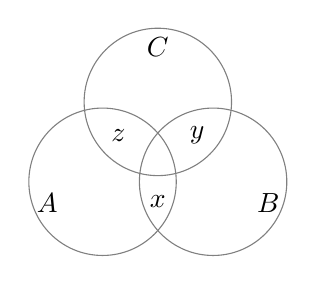
\begin{tikzpicture}[scale=0.78]
\draw[gray] (0,0.75) circle (1.2);
\draw[gray] (-0.9,-0.55) circle (1.2);
\draw[gray] (0.9,-0.55) circle (1.2);
\node at (0,1.65) {$C$};
\node at (-1.8,-0.9) {$A$};
\node at (1.8,-0.9) {$B$};
\node at (-0.64,0.20) {$z$};
\node at (0.64,0.20) {$y$};
\node at (0,-0.88) {$x$};
\end{tikzpicture}
\end{center}
\step{① 集合 $\{1,2,3,4\}$ 中的子集合有 4 个元素，所以从 $1,2,3,4$ 四个元素选 3 个有 $C_4^3=4$ 种方法，将 3 个元素进行全排列有 $P_3^3=3\times2=6$ 种，剩余的一个元素可以分别放入集合 $A$、$B$、$C$，有 3 种，所以此时共有 $3\times4\times6=72$ 种。}
\step{② 集合 $\{1,2,3,4\}$ 中的子集合有 3 个元素，满足集合 $A$、$B$、$C$ 中都只有一个元素。}
\step{所以从 $1,2,3,4$ 四个元素选 3 个有 $C_4^3=4$ 种方法，将 3 个元素进行全排列有 $P_3^3=3\times2=6$ 种，所以此时共有 $4\times6=24$ 种。}
\step{综上，共有 $72+24=96$ 个。}
\solend
\fi

\item 设 $a\in\R$，记 $f(x)=x^2+2x+a$，若关于 $x$ 的不等式 $f(f(x))<0$ 的解集为 $\varnothing$，则 $a$ 的取值范围为 \blankline[4.4em].

\ifanswer
\solbegin
\step{二次函数 $f(x)=x^2+2x+a$ 的开口向上，对称轴为 $x=-1$，所以 $f(x)_{\min}=f(-1)=a-1$，即 $f(x)$ 的值域为 $[a-1,+\infty)$.}
\step{要使不等式 $f(f(x))<0$ 的解集为空集，则 $f(f(x))\geqslant0$ 恒成立，}
\step{所以 $\begin{cases}f(a-1)\geqslant0,\\a-1\geqslant-1,\end{cases}$ 即 $\begin{cases}a^2+a-1\geqslant0,\\a\geqslant0,\end{cases}$}
\step{解得 $a\geqslant\dfrac{\sqrt5-1}{2}$，所以实数 $a$ 的取值范围为 $\left[\dfrac{\sqrt5-1}{2},+\infty\right)$.}
\solend
\fi

\end{enumerate}

\bigsec{二、选择题}

\begin{enumerate}
\setcounter{enumi}{12}

\item 已知关于 $x$ 的不等式 $2x-1>a(x-2)$ 的解集是 $\R$，则数 $a$ 的取值范围是\mbox{（\quad）}

\keepwithprev
A. $a>2$\qquad B. $a=2$

C. $a<2$\qquad D. $a$ 不存在

\ans{$B$}

\item 设 $0<a_1<a_2$，$0<b_1<b_2$，且 $a_1+a_2=b_1+b_2=1$，如果要把 $a_1b_1+a_2b_2$、$a_1b_2+a_2b_1$、$\dfrac12$ 按从小到大的顺序排列，那么排在中间的数是\mbox{（\quad）}

\keepwithprev
A. 一定是 $a_1b_1+a_2b_2$\qquad B. 一定是 $a_1b_2+a_2b_1$

C. 一定是 $\dfrac12$\qquad D. 不能确定，与 $a_1,a_2,b_1,b_2$ 的值有关

\ans{$C$}

\item “$0<a<b$”是“$a-\dfrac1a<b-\dfrac1b$”的\mbox{（\quad）}条件

\keepwithprev
A. 充分不必要\qquad B. 必要不充分

C. 充分必要\qquad D. 既不充分也不必要

\ans{$A$}

\item 在 $n$ 元集合 $S=\{a_1,a_2,\cdots,a_n\}$ 中，设 $x(S)=\dfrac{a_1+a_2+\cdots+a_n}{n}$，若 $S$ 的非空子集 $A$ 满足 $x(A)=x(S)$，则称 $A$ 是集合 $S$ 的一个“平均子集”，并记集合 $S$ 的 $k$ 个“平均子集”的个数为 $f_S(k)$. 已知集合 $S=\{1,2,3,4,5,6,7,8,9\}$，$T=\{-4,-3,-2,-1,0,1,2,3,4\}$，则下列说法错误的是\mbox{（\quad）}

\keepwithprev
A. $f_S(9)=f_T(1)$\qquad B. $f_S(8)=f_T(1)$

C. $f_S(6)=f_T(4)$\qquad D. $f_S(5)=f_T(4)$

\ans{$D$}

\ifanswer
\solbegin
\step{$X(S)=5$，将 $S$ 中的元素分成 5 组 $(1,9)$、$(2,8)$、$(3,7)$、$(4,6)$、$(5)$.}
\step{则 $f_S(1)=C_1^1=1$，$f_S(2)=C_4^1=4$，$f_S(3)=C_1^1C_4^1=4$，$f_S(4)=C_4^2=6$，$f_S(5)=C_1^1C_4^2=6$，同时 $X(T)=0$，将 $T$ 中的元素分成 5 组 $(1,-1)$、$(2,-2)$、$(3,-3)$、$(4,-4)$、$(0)$.}
\step{则 $f_T(1)=C_1^1=1$，$f_T(2)=C_4^1=4$，$f_T(3)=C_1^1C_4^1=4$，$f_T(4)=C_4^2=6$，$f_T(5)=C_1^1C_4^2=6$，$f_T(8)=C_4^4=1$，所以 $f_S(4)=f_S(5)=f_T(4)=6$，故选 D.}
\solend
\fi

\end{enumerate}

\bigsec{三、解答题}

\begin{enumerate}
\setcounter{enumi}{16}

\item 已知集合 $A=\{x\mid x^2-12x+20\leqslant0\}$，$B=\{x\mid2m<x<m+4\}$.

\begin{enumerate}[label=(\arabic*)]
\item 若 $m=3$，求 $A\cup B$；
\item 若 $A\cap B=\varnothing$，求 $m$ 的取值范围.
\end{enumerate}

\ifanswer
\solbegin
\stepm{(1)}{因为 $A=\{x\mid x^2-12x+20\leqslant0\}=\{x\mid2\leqslant x\leqslant10\}$，当 $m=3$ 时，$B=\{x\mid6<x<7\}$，所以 $A\cup B=\{x\mid2\leqslant x\leqslant10\}$.}
\stepm{(2)}{当 $m+4\leqslant2$ 时，$B$ 在 $A$ 的左侧，得 $m\leqslant-2$；当 $2m\geqslant10$ 时，得 $m\geqslant5$；当 $2m\geqslant m+4$ 时，$B=\varnothing$，得 $m\geqslant4$.}
\step{综上，$m\leqslant-2$ 或 $m\geqslant4$.}
\solend
\fi

\item 已知 $a>0$，关于 $x$ 的方程 $\dfrac1{x-2}+\dfrac1{x-1}=\dfrac{\sqrt{ax}}{x^2-3x+2}$ 有且仅有一个实数根，求实数 $a$ 的取值范围.

\ifanswer
\solbegin
\step{由题意得 $x\neq2$，$x\neq1$. 去分母整理得 $2x-3=\sqrt{ax}\geqslant0$，所以 $x\geqslant\dfrac32$，且 $x\neq2$.}
\step{两边平方整理得 $4x^2-(12+a)x+9=0$，判别式 $\Delta=a^2+24a>0$.}
\step{设方程的两个根为 $x_1$、$x_2$，则 $x_1+x_2=\dfrac{12+a}{4}$，$x_1x_2=\dfrac94$.}
\step{当 $0<a<\dfrac12$ 时，方程有一个根在 $\left(\dfrac32,2\right)$ 内，另一个根小于 $\dfrac32$，符合题意；}
\step{当 $a=\dfrac12$ 时，方程的根为 $2$、$\dfrac98$，均不符合题意；}
\step{当 $a>\dfrac12$ 时，方程有一个根大于 $2$，另一个根小于 $\dfrac32$，符合题意。}
\step{综上，实数 $a$ 的取值范围为 $\left(0,\dfrac12\right)\cup\left(\dfrac12,+\infty\right)$.}
\solend
\fi

\item 已知 $a\in\R$，关于 $x$ 的不等式 $ax^2-ax+3>0$ 恒成立.

\begin{enumerate}[label=(\arabic*)]
\item 求实数 $a$ 的取值范围；
\item 在（1）的条件下用反证法证明：三个关于 $x$ 的方程 $x^2+4ax-4a+3=0$，$x^2+(a-1)x+a^2=0$，$x^2+2ax-2a=0$ 中至少有一个方程有实数解.
\end{enumerate}

\ifanswer
\solbegin
\stepm{(1)}{当 $a=0$ 时，$3>0$ 恒成立；当 $a>0$ 时，$\Delta=a^2-12a<0$，解得 $0<a<12$；当 $a<0$ 时，不等式不恒成立。}
\step{综上，$a\in[0,12)$.}
\stepm{(2)}{假设三个方程均无实数解，则}
\step{$\begin{cases}\Delta_1=16a^2+16a-12<0,\\\Delta_2=(a-1)^2-4a^2<0,\\\Delta_3=4a^2+8a<0,\end{cases}$}
\step{解得 $-\dfrac32<a<\dfrac12$，$a<-1$ 或 $a>\dfrac13$，$-2<a<0$.}
\step{由 $a\in[0,12)$，前两个不等式得 $\dfrac13<a<\dfrac12$，第三个不等式得 $-2<a<0$，矛盾。}
\step{所以三个方程中至少有一个方程有实数解。}
\solend
\fi

% 注：原卷条件③按字面未限定 2x∈P_n；若对所有 x∈P_n 都要求 2x∈A，原卷答案 f(4)=4 与之不符。
%     2012 年江苏卷源题将其表述为相对于 P_n 的补集条件；本稿仍照录高一42原文，未替换。
\item 设集合 $P_n=\{1,2,\cdots,n\}$，$n\in\N^*$. 记 $f(n)$ 为同时满足下列条件的集合 $A$ 的个数：

① $A\subseteq P_n$；②若 $x\in A$，则 $2x\notin A$；③若 $x\notin A$，则 $2x\in A$.

\begin{enumerate}[label=(\arabic*)]
\item 求 $f(4)$；
\item 求 $f(n)$ 的解析式（用 $n$ 表示）.
\end{enumerate}

\ifanswer
\solbegin
\stepm{(1)}{当 $n=4$ 时，$P_4=\{1,2,3,4\}$，符合条件的集合 $A$ 为 $\{2\}$、$\{1,4\}$、$\{2,3\}$、$\{1,3,4\}$，故 $f(4)=4$.}
\stepm{(2)}{任取偶数 $x\in P_n$，将 $x$ 除以 2，若商仍为偶数，再除以 2，经过 $k$ 次后商必为奇数，此时商记为 $m$.}
\step{于是 $x=m\cdot2^k$，其中 $m$ 为奇数，$k\in\N^*$.}
\step{由条件得，若 $m\in A$，则 $x\in A\Longleftrightarrow k$ 为偶数；若 $m\notin A$，则 $x\in A\Longleftrightarrow k$ 为奇数。}
\step{因此每个奇数 $m\in P_n$ 是否属于 $A$ 可任意选择，且确定后其所有倍数的归属也唯一确定。}
\step{当 $n$ 为偶数时，$P_n$ 中奇数有 $\dfrac n2$ 个；当 $n$ 为奇数时，$P_n$ 中奇数有 $\dfrac{n+1}{2}$ 个。}
\step{所以 $f(n)=\begin{cases}2^{\frac n2},&n\text{ 为偶数},\\2^{\frac{n+1}{2}},&n\text{ 为奇数} .\end{cases}$}
\solend
\fi

\item 设 $S_n=\{(x_1,x_2,\cdots,x_n)\mid x_i\in\{0,1\},\ i=1,2,\cdots,n\}$（$n$ 为正整数），对任意的 $\alpha=(x_1,x_2,\cdots,x_n)$，$\beta=(y_1,y_2,\cdots,y_n)$，定义 $\alpha\cdot\beta=x_1y_1+x_2y_2+\cdots+x_ny_n$.

\begin{enumerate}[label=(\arabic*)]
\item 当 $n=3$ 时，$\alpha=(1,1,0)$，$\beta=(1,0,1)$，求 $\alpha\cdot\beta$；
\item 当 $n=3$ 时，集合 $A\subseteq S_n$，对任意 $\alpha,\beta\in A$，$\alpha\cdot\beta$ 均为偶数，求 $A$ 中元素个数的最大值；
\item 集合 $A\subseteq S_n$，对任意 $\alpha,\beta\in A$，$\alpha\neq\beta$，均有 $\alpha\cdot\beta\neq0$，求 $A$ 中元素个数的最大值.
\end{enumerate}

\ifanswer
\solbegin
\stepm{(1)}{当 $n=3$ 时，$\alpha\cdot\beta=x_1y_1+x_2y_2+x_3y_3=1\times1+1\times0+0\times1=1$.}
\stepm{(2)}{因为 $\alpha\cdot\beta=x_1y_1+x_2y_2+x_3y_3$ 均为偶数，所以结果为 $0$ 或 $2$.}
\step{当 $\alpha\cdot\beta=0$，则 $A$ 中元素个数最多有 $4$ 个；当 $\alpha\cdot\beta=2$，则 $A$ 中元素个数最多有 $1$ 个。}
\step{综上，$A$ 中元素个数的最大值为 $4$.}
\stepm{(3)}{若 $\alpha=(x_1,x_2,\cdots,x_n)\in A$，令 $\gamma=(1-x_1,1-x_2,\cdots,1-x_n)$，则 $\alpha\cdot\gamma=0$.}
\step{因为 $\alpha\cdot\beta\neq0$，$\alpha\in A$，所以 $\gamma\notin A$.}
\step{因为 $S_n$ 中有 $2^n$ 个元素，所以 $A$ 中元素个数最多有 $\dfrac{2^n}{2}=2^{n-1}$ 个。}
\step{综上，$A$ 中元素个数的最大值为 $2^{n-1}$.}
\solend
\fi

\end{enumerate}

\end{document}
"
% 紧凑版：xelatex "\def\iscompact{1}% 高一42_复旦附中_周末作业4.tex
%   —— 高一上数学“2026-2027 年复旦附中高一上周末作业 4”（试卷版/答案版）
% 试卷版：xelatex 高一42_复旦附中_周末作业4.tex
% 答案版：xelatex "\def\isanswer{1}\input{高一42_复旦附中_周末作业4.tex}"
% 紧凑版：xelatex "\def\iscompact{1}\input{高一42_复旦附中_周末作业4.tex}"
%
% 原始材料：微信公众号“魔都数学加油站”文章，作者破晓，2026-10-01 21:37 发布；
% 文章标题“27学年高一42——2026-2027年上海市复旦附中高一上周末作业4”；
% URL：https://mp.weixin.qq.com/s/nZ8aTd6K9OLS9S4-J-O7lA。
% 正文为 8 张 PNG 页（第 02、08 页 2560×3620，其余六页 4762×6735）。题目、答案及解析均据原图转录。
%
% 卷面标题行印作“2026-2027 年复旦附中高一上周末作业 4”，未印“上海市”；本稿标题照卷面，
% 年份区间按全稿惯例排 en dash。卷面未印副标题，本稿按“知识模块”口径标为“集合与常用逻辑用语、不等式”。
%
% 与原卷的排版差异：
%   ① 原文题号从第 3 题开始，本稿保留原题号；
%   ② 原卷的“一、填空题”“二、选择题”“三、解答题”改排为全稿统一的大节标题；
%   ③ 原卷填空横线统一排为 \blankline[4.4em]；选择题答案统一用 \ans{} 排在选项之后，
%      答案版与试卷版分离；原卷题目下方印出的【答案】、【解析】在答案版中排出；
%   ④ 原卷的粉色斜水印“魔都数学加油站”未录入；第 11 题解析中的三集合示意图以 TikZ 重绘。
%
% 原卷存疑处（照录原文）：
%   ① 第 5 题印出的答案为 $P>Q$，但取 $a=8,b=1$ 即得 $P=1<Q=\sqrt[3]{7}$；本稿照录；
%   ② 第 16 题解析按对称数对计数，印出 f_T(4)=C_4^2=6 并据此“故选 D”；但 T 中还可见
%      {0,1,2,-3} 这类和为 0 的四元子集，原卷的计数及选项结论疑有遗漏，本稿保留原解析和答案；
%   ③ 第 20 题的条件③印作“若 x∉A，则 2x∈A”，未明确限定 2x∈P_n；按此字面读法，f(4)
%      与【解析】列出的四个集合不符，而原题源 2012 年江苏卷明确写补集相对 P_n。
%      本稿照录原卷，不改条件，也不以源题替换；
%   ④ 第 21(2) 题题干未写 α≠β，解析结论为 4；此处照卷面题干与结论录入。
\documentclass[a4paper,11pt]{article}
\usepackage{common}

\begin{document}

\examtitlest[4]{2026--2027 年复旦附中高一上周末作业 4}{集合与常用逻辑用语、不等式}

\bigsec{一、填空题}

\begin{enumerate}
\setcounter{enumi}{2}

\item 若 $-1<x<y<2$，则 $x-y$ 的取值范围为 \blankline[4.4em].

\ifanswer
\solbegin
\step{$(-3,0)$.}
\solend
\fi

\item 已知 $c>d$，若 $ac+bd>bc+ad$，则 $a-b$ 与 $0$ 的大小关系是 \blankline[4.4em].

\ifanswer
\solbegin
\step{$a-b>0$.}
\solend
\fi

\item 已知 $a>b>0$，$P=\sqrt[3]{a}-\sqrt[3]{b}$，$Q=\sqrt[3]{a-b}$，则 $P$、$Q$ 的大小关系是 \blankline[4.4em].

\ifanswer
\solbegin
\step{$P>Q$.}
\solend
\fi

\item 对任意的实数 $x$，不等式 $x+|x-1|\geqslant m$ 恒成立，则实数 $m$ 的取值范围是 \blankline[4.4em].

\ifanswer
\solbegin
\step{令 $f(x)=x+|x-1|=\begin{cases}2x-1,&x\geqslant1,\\1,&x<1.\end{cases}$}
\step{当 $x\geqslant1$ 时，不等式变为 $2x-1\geqslant m$，显然满足题意；}
\step{当 $x<1$ 时，不等式变为 $1\geqslant m$，解得 $m\leqslant1$.}
\step{综上，$m\leqslant1$.}
\solend
\fi

\item 若“存在 $x\in\{x\mid1\leqslant x\leqslant2\}$，使得 $3x+a+1\geqslant0$”是命题，则实数 $a$ 的取值范围是 \blankline[4.4em].

\ifanswer
\solbegin
\step{由题意得 $6+a+1\geqslant0$，所以 $a\geqslant-7$.}
\solend
\fi

\item 已知关于 $x$ 的不等式 $ax-b\leqslant0$ 的解集是 $[2,+\infty)$，则关于 $x$ 的不等式
$ax^2+(3a-b)x-3b<0$ 的解集是 \blankline[4.4em].

\ifanswer
\solbegin
\step{由题意得 $a<0$，且 $\dfrac ba=2$，所以 $b=2a$.}
\step{当 $a<0$ 时，$ax^2+(3a-b)x-3b<0$ 等价于 $x^2+x-6>0$，}
\step{解得 $x\in(-\infty,-3)\cup(2,+\infty)$.}
\solend
\fi

\item 若关于 $x$ 的不等式 $(k^2+4k-5)x^2+4(1-k)x+3>0$ 恒成立，则实数 $k$ 的取值范围是 \blankline[4.4em].

\ifanswer
\solbegin
\step{当 $k=-5$ 时，不等式变为 $24x+3>0$，显然不满足题意，所以 $k\neq-5$.}
\step{当 $k=1$ 时，不等式变为 $3>0$，显然满足题意，所以 $k=1$.}
\step{当 $k^2+4k-5\neq0$ 时，有 $\begin{cases}k^2+4k-5>0,\\\Delta<0,\end{cases}$}
\step{即 $\begin{cases}k^2+4k-5>0,\\4(k-1)(k-19)<0,\end{cases}$，解得 $1<k<19$.}
\step{综上，实数 $k$ 的取值范围是 $[1,19)$.}
\solend
\fi

\item 设 $a\in\R$，集合 $A=\{x\mid x^2-ax+a\leqslant0\}$，若 $A\cap\N\neq\varnothing$，则 $a$ 的取值范围是 \blankline[4.4em].

\ifanswer
\solbegin
\step{$(-\infty,0]\cup[4,+\infty)$.}
\solend
\fi

\item 用 $|S|$ 表示集合 $S$ 中的元素的个数，设 $A$、$B$、$C$ 为集合，称 $(A,B,C)$ 为有序三元组。如果集合 $A$、$B$、$C$ 满足 $|A\cap B|=|B\cap C|=|C\cap A|=1$，且 $|A\cap B\cap C|=0$，则称有序三元组 $(A,B,C)$ 为最小交。由集合 $\{1,2,3,4\}$ 的子集构成的所有有序三元组中，最小交的有序三元组的个数为 \blankline[4.4em].

\ifanswer
\solbegin
\step{设 $A\cap B=\{x\}$，$B\cap C=\{y\}$，$C\cap A=\{z\}$，则 $x,y,z\in\{1,2,3,4\}$，且 $x,y,z$ 互不相同。}
\begin{center}
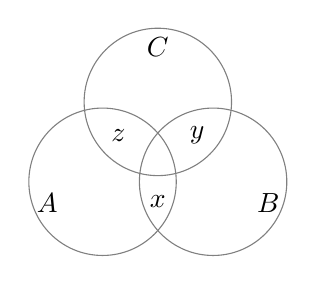
\begin{tikzpicture}[scale=0.78]
\draw[gray] (0,0.75) circle (1.2);
\draw[gray] (-0.9,-0.55) circle (1.2);
\draw[gray] (0.9,-0.55) circle (1.2);
\node at (0,1.65) {$C$};
\node at (-1.8,-0.9) {$A$};
\node at (1.8,-0.9) {$B$};
\node at (-0.64,0.20) {$z$};
\node at (0.64,0.20) {$y$};
\node at (0,-0.88) {$x$};
\end{tikzpicture}
\end{center}
\step{① 集合 $\{1,2,3,4\}$ 中的子集合有 4 个元素，所以从 $1,2,3,4$ 四个元素选 3 个有 $C_4^3=4$ 种方法，将 3 个元素进行全排列有 $P_3^3=3\times2=6$ 种，剩余的一个元素可以分别放入集合 $A$、$B$、$C$，有 3 种，所以此时共有 $3\times4\times6=72$ 种。}
\step{② 集合 $\{1,2,3,4\}$ 中的子集合有 3 个元素，满足集合 $A$、$B$、$C$ 中都只有一个元素。}
\step{所以从 $1,2,3,4$ 四个元素选 3 个有 $C_4^3=4$ 种方法，将 3 个元素进行全排列有 $P_3^3=3\times2=6$ 种，所以此时共有 $4\times6=24$ 种。}
\step{综上，共有 $72+24=96$ 个。}
\solend
\fi

\item 设 $a\in\R$，记 $f(x)=x^2+2x+a$，若关于 $x$ 的不等式 $f(f(x))<0$ 的解集为 $\varnothing$，则 $a$ 的取值范围为 \blankline[4.4em].

\ifanswer
\solbegin
\step{二次函数 $f(x)=x^2+2x+a$ 的开口向上，对称轴为 $x=-1$，所以 $f(x)_{\min}=f(-1)=a-1$，即 $f(x)$ 的值域为 $[a-1,+\infty)$.}
\step{要使不等式 $f(f(x))<0$ 的解集为空集，则 $f(f(x))\geqslant0$ 恒成立，}
\step{所以 $\begin{cases}f(a-1)\geqslant0,\\a-1\geqslant-1,\end{cases}$ 即 $\begin{cases}a^2+a-1\geqslant0,\\a\geqslant0,\end{cases}$}
\step{解得 $a\geqslant\dfrac{\sqrt5-1}{2}$，所以实数 $a$ 的取值范围为 $\left[\dfrac{\sqrt5-1}{2},+\infty\right)$.}
\solend
\fi

\end{enumerate}

\bigsec{二、选择题}

\begin{enumerate}
\setcounter{enumi}{12}

\item 已知关于 $x$ 的不等式 $2x-1>a(x-2)$ 的解集是 $\R$，则数 $a$ 的取值范围是\mbox{（\quad）}

\keepwithprev
A. $a>2$\qquad B. $a=2$

C. $a<2$\qquad D. $a$ 不存在

\ans{$B$}

\item 设 $0<a_1<a_2$，$0<b_1<b_2$，且 $a_1+a_2=b_1+b_2=1$，如果要把 $a_1b_1+a_2b_2$、$a_1b_2+a_2b_1$、$\dfrac12$ 按从小到大的顺序排列，那么排在中间的数是\mbox{（\quad）}

\keepwithprev
A. 一定是 $a_1b_1+a_2b_2$\qquad B. 一定是 $a_1b_2+a_2b_1$

C. 一定是 $\dfrac12$\qquad D. 不能确定，与 $a_1,a_2,b_1,b_2$ 的值有关

\ans{$C$}

\item “$0<a<b$”是“$a-\dfrac1a<b-\dfrac1b$”的\mbox{（\quad）}条件

\keepwithprev
A. 充分不必要\qquad B. 必要不充分

C. 充分必要\qquad D. 既不充分也不必要

\ans{$A$}

\item 在 $n$ 元集合 $S=\{a_1,a_2,\cdots,a_n\}$ 中，设 $x(S)=\dfrac{a_1+a_2+\cdots+a_n}{n}$，若 $S$ 的非空子集 $A$ 满足 $x(A)=x(S)$，则称 $A$ 是集合 $S$ 的一个“平均子集”，并记集合 $S$ 的 $k$ 个“平均子集”的个数为 $f_S(k)$. 已知集合 $S=\{1,2,3,4,5,6,7,8,9\}$，$T=\{-4,-3,-2,-1,0,1,2,3,4\}$，则下列说法错误的是\mbox{（\quad）}

\keepwithprev
A. $f_S(9)=f_T(1)$\qquad B. $f_S(8)=f_T(1)$

C. $f_S(6)=f_T(4)$\qquad D. $f_S(5)=f_T(4)$

\ans{$D$}

\ifanswer
\solbegin
\step{$X(S)=5$，将 $S$ 中的元素分成 5 组 $(1,9)$、$(2,8)$、$(3,7)$、$(4,6)$、$(5)$.}
\step{则 $f_S(1)=C_1^1=1$，$f_S(2)=C_4^1=4$，$f_S(3)=C_1^1C_4^1=4$，$f_S(4)=C_4^2=6$，$f_S(5)=C_1^1C_4^2=6$，同时 $X(T)=0$，将 $T$ 中的元素分成 5 组 $(1,-1)$、$(2,-2)$、$(3,-3)$、$(4,-4)$、$(0)$.}
\step{则 $f_T(1)=C_1^1=1$，$f_T(2)=C_4^1=4$，$f_T(3)=C_1^1C_4^1=4$，$f_T(4)=C_4^2=6$，$f_T(5)=C_1^1C_4^2=6$，$f_T(8)=C_4^4=1$，所以 $f_S(4)=f_S(5)=f_T(4)=6$，故选 D.}
\solend
\fi

\end{enumerate}

\bigsec{三、解答题}

\begin{enumerate}
\setcounter{enumi}{16}

\item 已知集合 $A=\{x\mid x^2-12x+20\leqslant0\}$，$B=\{x\mid2m<x<m+4\}$.

\begin{enumerate}[label=(\arabic*)]
\item 若 $m=3$，求 $A\cup B$；
\item 若 $A\cap B=\varnothing$，求 $m$ 的取值范围.
\end{enumerate}

\ifanswer
\solbegin
\stepm{(1)}{因为 $A=\{x\mid x^2-12x+20\leqslant0\}=\{x\mid2\leqslant x\leqslant10\}$，当 $m=3$ 时，$B=\{x\mid6<x<7\}$，所以 $A\cup B=\{x\mid2\leqslant x\leqslant10\}$.}
\stepm{(2)}{当 $m+4\leqslant2$ 时，$B$ 在 $A$ 的左侧，得 $m\leqslant-2$；当 $2m\geqslant10$ 时，得 $m\geqslant5$；当 $2m\geqslant m+4$ 时，$B=\varnothing$，得 $m\geqslant4$.}
\step{综上，$m\leqslant-2$ 或 $m\geqslant4$.}
\solend
\fi

\item 已知 $a>0$，关于 $x$ 的方程 $\dfrac1{x-2}+\dfrac1{x-1}=\dfrac{\sqrt{ax}}{x^2-3x+2}$ 有且仅有一个实数根，求实数 $a$ 的取值范围.

\ifanswer
\solbegin
\step{由题意得 $x\neq2$，$x\neq1$. 去分母整理得 $2x-3=\sqrt{ax}\geqslant0$，所以 $x\geqslant\dfrac32$，且 $x\neq2$.}
\step{两边平方整理得 $4x^2-(12+a)x+9=0$，判别式 $\Delta=a^2+24a>0$.}
\step{设方程的两个根为 $x_1$、$x_2$，则 $x_1+x_2=\dfrac{12+a}{4}$，$x_1x_2=\dfrac94$.}
\step{当 $0<a<\dfrac12$ 时，方程有一个根在 $\left(\dfrac32,2\right)$ 内，另一个根小于 $\dfrac32$，符合题意；}
\step{当 $a=\dfrac12$ 时，方程的根为 $2$、$\dfrac98$，均不符合题意；}
\step{当 $a>\dfrac12$ 时，方程有一个根大于 $2$，另一个根小于 $\dfrac32$，符合题意。}
\step{综上，实数 $a$ 的取值范围为 $\left(0,\dfrac12\right)\cup\left(\dfrac12,+\infty\right)$.}
\solend
\fi

\item 已知 $a\in\R$，关于 $x$ 的不等式 $ax^2-ax+3>0$ 恒成立.

\begin{enumerate}[label=(\arabic*)]
\item 求实数 $a$ 的取值范围；
\item 在（1）的条件下用反证法证明：三个关于 $x$ 的方程 $x^2+4ax-4a+3=0$，$x^2+(a-1)x+a^2=0$，$x^2+2ax-2a=0$ 中至少有一个方程有实数解.
\end{enumerate}

\ifanswer
\solbegin
\stepm{(1)}{当 $a=0$ 时，$3>0$ 恒成立；当 $a>0$ 时，$\Delta=a^2-12a<0$，解得 $0<a<12$；当 $a<0$ 时，不等式不恒成立。}
\step{综上，$a\in[0,12)$.}
\stepm{(2)}{假设三个方程均无实数解，则}
\step{$\begin{cases}\Delta_1=16a^2+16a-12<0,\\\Delta_2=(a-1)^2-4a^2<0,\\\Delta_3=4a^2+8a<0,\end{cases}$}
\step{解得 $-\dfrac32<a<\dfrac12$，$a<-1$ 或 $a>\dfrac13$，$-2<a<0$.}
\step{由 $a\in[0,12)$，前两个不等式得 $\dfrac13<a<\dfrac12$，第三个不等式得 $-2<a<0$，矛盾。}
\step{所以三个方程中至少有一个方程有实数解。}
\solend
\fi

% 注：原卷条件③按字面未限定 2x∈P_n；若对所有 x∈P_n 都要求 2x∈A，原卷答案 f(4)=4 与之不符。
%     2012 年江苏卷源题将其表述为相对于 P_n 的补集条件；本稿仍照录高一42原文，未替换。
\item 设集合 $P_n=\{1,2,\cdots,n\}$，$n\in\N^*$. 记 $f(n)$ 为同时满足下列条件的集合 $A$ 的个数：

① $A\subseteq P_n$；②若 $x\in A$，则 $2x\notin A$；③若 $x\notin A$，则 $2x\in A$.

\begin{enumerate}[label=(\arabic*)]
\item 求 $f(4)$；
\item 求 $f(n)$ 的解析式（用 $n$ 表示）.
\end{enumerate}

\ifanswer
\solbegin
\stepm{(1)}{当 $n=4$ 时，$P_4=\{1,2,3,4\}$，符合条件的集合 $A$ 为 $\{2\}$、$\{1,4\}$、$\{2,3\}$、$\{1,3,4\}$，故 $f(4)=4$.}
\stepm{(2)}{任取偶数 $x\in P_n$，将 $x$ 除以 2，若商仍为偶数，再除以 2，经过 $k$ 次后商必为奇数，此时商记为 $m$.}
\step{于是 $x=m\cdot2^k$，其中 $m$ 为奇数，$k\in\N^*$.}
\step{由条件得，若 $m\in A$，则 $x\in A\Longleftrightarrow k$ 为偶数；若 $m\notin A$，则 $x\in A\Longleftrightarrow k$ 为奇数。}
\step{因此每个奇数 $m\in P_n$ 是否属于 $A$ 可任意选择，且确定后其所有倍数的归属也唯一确定。}
\step{当 $n$ 为偶数时，$P_n$ 中奇数有 $\dfrac n2$ 个；当 $n$ 为奇数时，$P_n$ 中奇数有 $\dfrac{n+1}{2}$ 个。}
\step{所以 $f(n)=\begin{cases}2^{\frac n2},&n\text{ 为偶数},\\2^{\frac{n+1}{2}},&n\text{ 为奇数} .\end{cases}$}
\solend
\fi

\item 设 $S_n=\{(x_1,x_2,\cdots,x_n)\mid x_i\in\{0,1\},\ i=1,2,\cdots,n\}$（$n$ 为正整数），对任意的 $\alpha=(x_1,x_2,\cdots,x_n)$，$\beta=(y_1,y_2,\cdots,y_n)$，定义 $\alpha\cdot\beta=x_1y_1+x_2y_2+\cdots+x_ny_n$.

\begin{enumerate}[label=(\arabic*)]
\item 当 $n=3$ 时，$\alpha=(1,1,0)$，$\beta=(1,0,1)$，求 $\alpha\cdot\beta$；
\item 当 $n=3$ 时，集合 $A\subseteq S_n$，对任意 $\alpha,\beta\in A$，$\alpha\cdot\beta$ 均为偶数，求 $A$ 中元素个数的最大值；
\item 集合 $A\subseteq S_n$，对任意 $\alpha,\beta\in A$，$\alpha\neq\beta$，均有 $\alpha\cdot\beta\neq0$，求 $A$ 中元素个数的最大值.
\end{enumerate}

\ifanswer
\solbegin
\stepm{(1)}{当 $n=3$ 时，$\alpha\cdot\beta=x_1y_1+x_2y_2+x_3y_3=1\times1+1\times0+0\times1=1$.}
\stepm{(2)}{因为 $\alpha\cdot\beta=x_1y_1+x_2y_2+x_3y_3$ 均为偶数，所以结果为 $0$ 或 $2$.}
\step{当 $\alpha\cdot\beta=0$，则 $A$ 中元素个数最多有 $4$ 个；当 $\alpha\cdot\beta=2$，则 $A$ 中元素个数最多有 $1$ 个。}
\step{综上，$A$ 中元素个数的最大值为 $4$.}
\stepm{(3)}{若 $\alpha=(x_1,x_2,\cdots,x_n)\in A$，令 $\gamma=(1-x_1,1-x_2,\cdots,1-x_n)$，则 $\alpha\cdot\gamma=0$.}
\step{因为 $\alpha\cdot\beta\neq0$，$\alpha\in A$，所以 $\gamma\notin A$.}
\step{因为 $S_n$ 中有 $2^n$ 个元素，所以 $A$ 中元素个数最多有 $\dfrac{2^n}{2}=2^{n-1}$ 个。}
\step{综上，$A$ 中元素个数的最大值为 $2^{n-1}$.}
\solend
\fi

\end{enumerate}

\end{document}
"
%
% 原始材料：微信公众号“魔都数学加油站”文章，作者破晓，2026-10-01 21:37 发布；
% 文章标题“27学年高一42——2026-2027年上海市复旦附中高一上周末作业4”；
% URL：https://mp.weixin.qq.com/s/nZ8aTd6K9OLS9S4-J-O7lA。
% 正文为 8 张 PNG 页（第 02、08 页 2560×3620，其余六页 4762×6735）。题目、答案及解析均据原图转录。
%
% 卷面标题行印作“2026-2027 年复旦附中高一上周末作业 4”，未印“上海市”；本稿标题照卷面，
% 年份区间按全稿惯例排 en dash。卷面未印副标题，本稿按“知识模块”口径标为“集合与常用逻辑用语、不等式”。
%
% 与原卷的排版差异：
%   ① 原文题号从第 3 题开始，本稿保留原题号；
%   ② 原卷的“一、填空题”“二、选择题”“三、解答题”改排为全稿统一的大节标题；
%   ③ 原卷填空横线统一排为 \blankline[4.4em]；选择题答案统一用 \ans{} 排在选项之后，
%      答案版与试卷版分离；原卷题目下方印出的【答案】、【解析】在答案版中排出；
%   ④ 原卷的粉色斜水印“魔都数学加油站”未录入；第 11 题解析中的三集合示意图以 TikZ 重绘。
%
% 原卷存疑处（照录原文）：
%   ① 第 5 题印出的答案为 $P>Q$，但取 $a=8,b=1$ 即得 $P=1<Q=\sqrt[3]{7}$；本稿照录；
%   ② 第 16 题解析按对称数对计数，印出 f_T(4)=C_4^2=6 并据此“故选 D”；但 T 中还可见
%      {0,1,2,-3} 这类和为 0 的四元子集，原卷的计数及选项结论疑有遗漏，本稿保留原解析和答案；
%   ③ 第 20 题的条件③印作“若 x∉A，则 2x∈A”，未明确限定 2x∈P_n；按此字面读法，f(4)
%      与【解析】列出的四个集合不符，而原题源 2012 年江苏卷明确写补集相对 P_n。
%      本稿照录原卷，不改条件，也不以源题替换；
%   ④ 第 21(2) 题题干未写 α≠β，解析结论为 4；此处照卷面题干与结论录入。
\documentclass[a4paper,11pt]{article}
\usepackage{common}

\begin{document}

\examtitlest[4]{2026--2027 年复旦附中高一上周末作业 4}{集合与常用逻辑用语、不等式}

\bigsec{一、填空题}

\begin{enumerate}
\setcounter{enumi}{2}

\item 若 $-1<x<y<2$，则 $x-y$ 的取值范围为 \blankline[4.4em].

\ifanswer
\solbegin
\step{$(-3,0)$.}
\solend
\fi

\item 已知 $c>d$，若 $ac+bd>bc+ad$，则 $a-b$ 与 $0$ 的大小关系是 \blankline[4.4em].

\ifanswer
\solbegin
\step{$a-b>0$.}
\solend
\fi

\item 已知 $a>b>0$，$P=\sqrt[3]{a}-\sqrt[3]{b}$，$Q=\sqrt[3]{a-b}$，则 $P$、$Q$ 的大小关系是 \blankline[4.4em].

\ifanswer
\solbegin
\step{$P>Q$.}
\solend
\fi

\item 对任意的实数 $x$，不等式 $x+|x-1|\geqslant m$ 恒成立，则实数 $m$ 的取值范围是 \blankline[4.4em].

\ifanswer
\solbegin
\step{令 $f(x)=x+|x-1|=\begin{cases}2x-1,&x\geqslant1,\\1,&x<1.\end{cases}$}
\step{当 $x\geqslant1$ 时，不等式变为 $2x-1\geqslant m$，显然满足题意；}
\step{当 $x<1$ 时，不等式变为 $1\geqslant m$，解得 $m\leqslant1$.}
\step{综上，$m\leqslant1$.}
\solend
\fi

\item 若“存在 $x\in\{x\mid1\leqslant x\leqslant2\}$，使得 $3x+a+1\geqslant0$”是命题，则实数 $a$ 的取值范围是 \blankline[4.4em].

\ifanswer
\solbegin
\step{由题意得 $6+a+1\geqslant0$，所以 $a\geqslant-7$.}
\solend
\fi

\item 已知关于 $x$ 的不等式 $ax-b\leqslant0$ 的解集是 $[2,+\infty)$，则关于 $x$ 的不等式
$ax^2+(3a-b)x-3b<0$ 的解集是 \blankline[4.4em].

\ifanswer
\solbegin
\step{由题意得 $a<0$，且 $\dfrac ba=2$，所以 $b=2a$.}
\step{当 $a<0$ 时，$ax^2+(3a-b)x-3b<0$ 等价于 $x^2+x-6>0$，}
\step{解得 $x\in(-\infty,-3)\cup(2,+\infty)$.}
\solend
\fi

\item 若关于 $x$ 的不等式 $(k^2+4k-5)x^2+4(1-k)x+3>0$ 恒成立，则实数 $k$ 的取值范围是 \blankline[4.4em].

\ifanswer
\solbegin
\step{当 $k=-5$ 时，不等式变为 $24x+3>0$，显然不满足题意，所以 $k\neq-5$.}
\step{当 $k=1$ 时，不等式变为 $3>0$，显然满足题意，所以 $k=1$.}
\step{当 $k^2+4k-5\neq0$ 时，有 $\begin{cases}k^2+4k-5>0,\\\Delta<0,\end{cases}$}
\step{即 $\begin{cases}k^2+4k-5>0,\\4(k-1)(k-19)<0,\end{cases}$，解得 $1<k<19$.}
\step{综上，实数 $k$ 的取值范围是 $[1,19)$.}
\solend
\fi

\item 设 $a\in\R$，集合 $A=\{x\mid x^2-ax+a\leqslant0\}$，若 $A\cap\N\neq\varnothing$，则 $a$ 的取值范围是 \blankline[4.4em].

\ifanswer
\solbegin
\step{$(-\infty,0]\cup[4,+\infty)$.}
\solend
\fi

\item 用 $|S|$ 表示集合 $S$ 中的元素的个数，设 $A$、$B$、$C$ 为集合，称 $(A,B,C)$ 为有序三元组。如果集合 $A$、$B$、$C$ 满足 $|A\cap B|=|B\cap C|=|C\cap A|=1$，且 $|A\cap B\cap C|=0$，则称有序三元组 $(A,B,C)$ 为最小交。由集合 $\{1,2,3,4\}$ 的子集构成的所有有序三元组中，最小交的有序三元组的个数为 \blankline[4.4em].

\ifanswer
\solbegin
\step{设 $A\cap B=\{x\}$，$B\cap C=\{y\}$，$C\cap A=\{z\}$，则 $x,y,z\in\{1,2,3,4\}$，且 $x,y,z$ 互不相同。}
\begin{center}
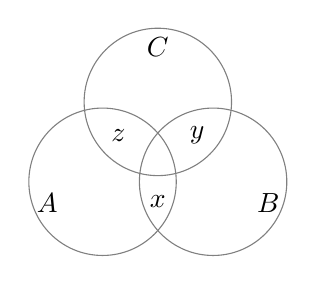
\begin{tikzpicture}[scale=0.78]
\draw[gray] (0,0.75) circle (1.2);
\draw[gray] (-0.9,-0.55) circle (1.2);
\draw[gray] (0.9,-0.55) circle (1.2);
\node at (0,1.65) {$C$};
\node at (-1.8,-0.9) {$A$};
\node at (1.8,-0.9) {$B$};
\node at (-0.64,0.20) {$z$};
\node at (0.64,0.20) {$y$};
\node at (0,-0.88) {$x$};
\end{tikzpicture}
\end{center}
\step{① 集合 $\{1,2,3,4\}$ 中的子集合有 4 个元素，所以从 $1,2,3,4$ 四个元素选 3 个有 $C_4^3=4$ 种方法，将 3 个元素进行全排列有 $P_3^3=3\times2=6$ 种，剩余的一个元素可以分别放入集合 $A$、$B$、$C$，有 3 种，所以此时共有 $3\times4\times6=72$ 种。}
\step{② 集合 $\{1,2,3,4\}$ 中的子集合有 3 个元素，满足集合 $A$、$B$、$C$ 中都只有一个元素。}
\step{所以从 $1,2,3,4$ 四个元素选 3 个有 $C_4^3=4$ 种方法，将 3 个元素进行全排列有 $P_3^3=3\times2=6$ 种，所以此时共有 $4\times6=24$ 种。}
\step{综上，共有 $72+24=96$ 个。}
\solend
\fi

\item 设 $a\in\R$，记 $f(x)=x^2+2x+a$，若关于 $x$ 的不等式 $f(f(x))<0$ 的解集为 $\varnothing$，则 $a$ 的取值范围为 \blankline[4.4em].

\ifanswer
\solbegin
\step{二次函数 $f(x)=x^2+2x+a$ 的开口向上，对称轴为 $x=-1$，所以 $f(x)_{\min}=f(-1)=a-1$，即 $f(x)$ 的值域为 $[a-1,+\infty)$.}
\step{要使不等式 $f(f(x))<0$ 的解集为空集，则 $f(f(x))\geqslant0$ 恒成立，}
\step{所以 $\begin{cases}f(a-1)\geqslant0,\\a-1\geqslant-1,\end{cases}$ 即 $\begin{cases}a^2+a-1\geqslant0,\\a\geqslant0,\end{cases}$}
\step{解得 $a\geqslant\dfrac{\sqrt5-1}{2}$，所以实数 $a$ 的取值范围为 $\left[\dfrac{\sqrt5-1}{2},+\infty\right)$.}
\solend
\fi

\end{enumerate}

\bigsec{二、选择题}

\begin{enumerate}
\setcounter{enumi}{12}

\item 已知关于 $x$ 的不等式 $2x-1>a(x-2)$ 的解集是 $\R$，则数 $a$ 的取值范围是\mbox{（\quad）}

\keepwithprev
A. $a>2$\qquad B. $a=2$

C. $a<2$\qquad D. $a$ 不存在

\ans{$B$}

\item 设 $0<a_1<a_2$，$0<b_1<b_2$，且 $a_1+a_2=b_1+b_2=1$，如果要把 $a_1b_1+a_2b_2$、$a_1b_2+a_2b_1$、$\dfrac12$ 按从小到大的顺序排列，那么排在中间的数是\mbox{（\quad）}

\keepwithprev
A. 一定是 $a_1b_1+a_2b_2$\qquad B. 一定是 $a_1b_2+a_2b_1$

C. 一定是 $\dfrac12$\qquad D. 不能确定，与 $a_1,a_2,b_1,b_2$ 的值有关

\ans{$C$}

\item “$0<a<b$”是“$a-\dfrac1a<b-\dfrac1b$”的\mbox{（\quad）}条件

\keepwithprev
A. 充分不必要\qquad B. 必要不充分

C. 充分必要\qquad D. 既不充分也不必要

\ans{$A$}

\item 在 $n$ 元集合 $S=\{a_1,a_2,\cdots,a_n\}$ 中，设 $x(S)=\dfrac{a_1+a_2+\cdots+a_n}{n}$，若 $S$ 的非空子集 $A$ 满足 $x(A)=x(S)$，则称 $A$ 是集合 $S$ 的一个“平均子集”，并记集合 $S$ 的 $k$ 个“平均子集”的个数为 $f_S(k)$. 已知集合 $S=\{1,2,3,4,5,6,7,8,9\}$，$T=\{-4,-3,-2,-1,0,1,2,3,4\}$，则下列说法错误的是\mbox{（\quad）}

\keepwithprev
A. $f_S(9)=f_T(1)$\qquad B. $f_S(8)=f_T(1)$

C. $f_S(6)=f_T(4)$\qquad D. $f_S(5)=f_T(4)$

\ans{$D$}

\ifanswer
\solbegin
\step{$X(S)=5$，将 $S$ 中的元素分成 5 组 $(1,9)$、$(2,8)$、$(3,7)$、$(4,6)$、$(5)$.}
\step{则 $f_S(1)=C_1^1=1$，$f_S(2)=C_4^1=4$，$f_S(3)=C_1^1C_4^1=4$，$f_S(4)=C_4^2=6$，$f_S(5)=C_1^1C_4^2=6$，同时 $X(T)=0$，将 $T$ 中的元素分成 5 组 $(1,-1)$、$(2,-2)$、$(3,-3)$、$(4,-4)$、$(0)$.}
\step{则 $f_T(1)=C_1^1=1$，$f_T(2)=C_4^1=4$，$f_T(3)=C_1^1C_4^1=4$，$f_T(4)=C_4^2=6$，$f_T(5)=C_1^1C_4^2=6$，$f_T(8)=C_4^4=1$，所以 $f_S(4)=f_S(5)=f_T(4)=6$，故选 D.}
\solend
\fi

\end{enumerate}

\bigsec{三、解答题}

\begin{enumerate}
\setcounter{enumi}{16}

\item 已知集合 $A=\{x\mid x^2-12x+20\leqslant0\}$，$B=\{x\mid2m<x<m+4\}$.

\begin{enumerate}[label=(\arabic*)]
\item 若 $m=3$，求 $A\cup B$；
\item 若 $A\cap B=\varnothing$，求 $m$ 的取值范围.
\end{enumerate}

\ifanswer
\solbegin
\stepm{(1)}{因为 $A=\{x\mid x^2-12x+20\leqslant0\}=\{x\mid2\leqslant x\leqslant10\}$，当 $m=3$ 时，$B=\{x\mid6<x<7\}$，所以 $A\cup B=\{x\mid2\leqslant x\leqslant10\}$.}
\stepm{(2)}{当 $m+4\leqslant2$ 时，$B$ 在 $A$ 的左侧，得 $m\leqslant-2$；当 $2m\geqslant10$ 时，得 $m\geqslant5$；当 $2m\geqslant m+4$ 时，$B=\varnothing$，得 $m\geqslant4$.}
\step{综上，$m\leqslant-2$ 或 $m\geqslant4$.}
\solend
\fi

\item 已知 $a>0$，关于 $x$ 的方程 $\dfrac1{x-2}+\dfrac1{x-1}=\dfrac{\sqrt{ax}}{x^2-3x+2}$ 有且仅有一个实数根，求实数 $a$ 的取值范围.

\ifanswer
\solbegin
\step{由题意得 $x\neq2$，$x\neq1$. 去分母整理得 $2x-3=\sqrt{ax}\geqslant0$，所以 $x\geqslant\dfrac32$，且 $x\neq2$.}
\step{两边平方整理得 $4x^2-(12+a)x+9=0$，判别式 $\Delta=a^2+24a>0$.}
\step{设方程的两个根为 $x_1$、$x_2$，则 $x_1+x_2=\dfrac{12+a}{4}$，$x_1x_2=\dfrac94$.}
\step{当 $0<a<\dfrac12$ 时，方程有一个根在 $\left(\dfrac32,2\right)$ 内，另一个根小于 $\dfrac32$，符合题意；}
\step{当 $a=\dfrac12$ 时，方程的根为 $2$、$\dfrac98$，均不符合题意；}
\step{当 $a>\dfrac12$ 时，方程有一个根大于 $2$，另一个根小于 $\dfrac32$，符合题意。}
\step{综上，实数 $a$ 的取值范围为 $\left(0,\dfrac12\right)\cup\left(\dfrac12,+\infty\right)$.}
\solend
\fi

\item 已知 $a\in\R$，关于 $x$ 的不等式 $ax^2-ax+3>0$ 恒成立.

\begin{enumerate}[label=(\arabic*)]
\item 求实数 $a$ 的取值范围；
\item 在（1）的条件下用反证法证明：三个关于 $x$ 的方程 $x^2+4ax-4a+3=0$，$x^2+(a-1)x+a^2=0$，$x^2+2ax-2a=0$ 中至少有一个方程有实数解.
\end{enumerate}

\ifanswer
\solbegin
\stepm{(1)}{当 $a=0$ 时，$3>0$ 恒成立；当 $a>0$ 时，$\Delta=a^2-12a<0$，解得 $0<a<12$；当 $a<0$ 时，不等式不恒成立。}
\step{综上，$a\in[0,12)$.}
\stepm{(2)}{假设三个方程均无实数解，则}
\step{$\begin{cases}\Delta_1=16a^2+16a-12<0,\\\Delta_2=(a-1)^2-4a^2<0,\\\Delta_3=4a^2+8a<0,\end{cases}$}
\step{解得 $-\dfrac32<a<\dfrac12$，$a<-1$ 或 $a>\dfrac13$，$-2<a<0$.}
\step{由 $a\in[0,12)$，前两个不等式得 $\dfrac13<a<\dfrac12$，第三个不等式得 $-2<a<0$，矛盾。}
\step{所以三个方程中至少有一个方程有实数解。}
\solend
\fi

% 注：原卷条件③按字面未限定 2x∈P_n；若对所有 x∈P_n 都要求 2x∈A，原卷答案 f(4)=4 与之不符。
%     2012 年江苏卷源题将其表述为相对于 P_n 的补集条件；本稿仍照录高一42原文，未替换。
\item 设集合 $P_n=\{1,2,\cdots,n\}$，$n\in\N^*$. 记 $f(n)$ 为同时满足下列条件的集合 $A$ 的个数：

① $A\subseteq P_n$；②若 $x\in A$，则 $2x\notin A$；③若 $x\notin A$，则 $2x\in A$.

\begin{enumerate}[label=(\arabic*)]
\item 求 $f(4)$；
\item 求 $f(n)$ 的解析式（用 $n$ 表示）.
\end{enumerate}

\ifanswer
\solbegin
\stepm{(1)}{当 $n=4$ 时，$P_4=\{1,2,3,4\}$，符合条件的集合 $A$ 为 $\{2\}$、$\{1,4\}$、$\{2,3\}$、$\{1,3,4\}$，故 $f(4)=4$.}
\stepm{(2)}{任取偶数 $x\in P_n$，将 $x$ 除以 2，若商仍为偶数，再除以 2，经过 $k$ 次后商必为奇数，此时商记为 $m$.}
\step{于是 $x=m\cdot2^k$，其中 $m$ 为奇数，$k\in\N^*$.}
\step{由条件得，若 $m\in A$，则 $x\in A\Longleftrightarrow k$ 为偶数；若 $m\notin A$，则 $x\in A\Longleftrightarrow k$ 为奇数。}
\step{因此每个奇数 $m\in P_n$ 是否属于 $A$ 可任意选择，且确定后其所有倍数的归属也唯一确定。}
\step{当 $n$ 为偶数时，$P_n$ 中奇数有 $\dfrac n2$ 个；当 $n$ 为奇数时，$P_n$ 中奇数有 $\dfrac{n+1}{2}$ 个。}
\step{所以 $f(n)=\begin{cases}2^{\frac n2},&n\text{ 为偶数},\\2^{\frac{n+1}{2}},&n\text{ 为奇数} .\end{cases}$}
\solend
\fi

\item 设 $S_n=\{(x_1,x_2,\cdots,x_n)\mid x_i\in\{0,1\},\ i=1,2,\cdots,n\}$（$n$ 为正整数），对任意的 $\alpha=(x_1,x_2,\cdots,x_n)$，$\beta=(y_1,y_2,\cdots,y_n)$，定义 $\alpha\cdot\beta=x_1y_1+x_2y_2+\cdots+x_ny_n$.

\begin{enumerate}[label=(\arabic*)]
\item 当 $n=3$ 时，$\alpha=(1,1,0)$，$\beta=(1,0,1)$，求 $\alpha\cdot\beta$；
\item 当 $n=3$ 时，集合 $A\subseteq S_n$，对任意 $\alpha,\beta\in A$，$\alpha\cdot\beta$ 均为偶数，求 $A$ 中元素个数的最大值；
\item 集合 $A\subseteq S_n$，对任意 $\alpha,\beta\in A$，$\alpha\neq\beta$，均有 $\alpha\cdot\beta\neq0$，求 $A$ 中元素个数的最大值.
\end{enumerate}

\ifanswer
\solbegin
\stepm{(1)}{当 $n=3$ 时，$\alpha\cdot\beta=x_1y_1+x_2y_2+x_3y_3=1\times1+1\times0+0\times1=1$.}
\stepm{(2)}{因为 $\alpha\cdot\beta=x_1y_1+x_2y_2+x_3y_3$ 均为偶数，所以结果为 $0$ 或 $2$.}
\step{当 $\alpha\cdot\beta=0$，则 $A$ 中元素个数最多有 $4$ 个；当 $\alpha\cdot\beta=2$，则 $A$ 中元素个数最多有 $1$ 个。}
\step{综上，$A$ 中元素个数的最大值为 $4$.}
\stepm{(3)}{若 $\alpha=(x_1,x_2,\cdots,x_n)\in A$，令 $\gamma=(1-x_1,1-x_2,\cdots,1-x_n)$，则 $\alpha\cdot\gamma=0$.}
\step{因为 $\alpha\cdot\beta\neq0$，$\alpha\in A$，所以 $\gamma\notin A$.}
\step{因为 $S_n$ 中有 $2^n$ 个元素，所以 $A$ 中元素个数最多有 $\dfrac{2^n}{2}=2^{n-1}$ 个。}
\step{综上，$A$ 中元素个数的最大值为 $2^{n-1}$.}
\solend
\fi

\end{enumerate}

\end{document}
"
% 紧凑版：xelatex "\def\iscompact{1}% 高一42_复旦附中_周末作业4.tex
%   —— 高一上数学“2026-2027 年复旦附中高一上周末作业 4”（试卷版/答案版）
% 试卷版：xelatex 高一42_复旦附中_周末作业4.tex
% 答案版：xelatex "\def\isanswer{1}% 高一42_复旦附中_周末作业4.tex
%   —— 高一上数学“2026-2027 年复旦附中高一上周末作业 4”（试卷版/答案版）
% 试卷版：xelatex 高一42_复旦附中_周末作业4.tex
% 答案版：xelatex "\def\isanswer{1}\input{高一42_复旦附中_周末作业4.tex}"
% 紧凑版：xelatex "\def\iscompact{1}\input{高一42_复旦附中_周末作业4.tex}"
%
% 原始材料：微信公众号“魔都数学加油站”文章，作者破晓，2026-10-01 21:37 发布；
% 文章标题“27学年高一42——2026-2027年上海市复旦附中高一上周末作业4”；
% URL：https://mp.weixin.qq.com/s/nZ8aTd6K9OLS9S4-J-O7lA。
% 正文为 8 张 PNG 页（第 02、08 页 2560×3620，其余六页 4762×6735）。题目、答案及解析均据原图转录。
%
% 卷面标题行印作“2026-2027 年复旦附中高一上周末作业 4”，未印“上海市”；本稿标题照卷面，
% 年份区间按全稿惯例排 en dash。卷面未印副标题，本稿按“知识模块”口径标为“集合与常用逻辑用语、不等式”。
%
% 与原卷的排版差异：
%   ① 原文题号从第 3 题开始，本稿保留原题号；
%   ② 原卷的“一、填空题”“二、选择题”“三、解答题”改排为全稿统一的大节标题；
%   ③ 原卷填空横线统一排为 \blankline[4.4em]；选择题答案统一用 \ans{} 排在选项之后，
%      答案版与试卷版分离；原卷题目下方印出的【答案】、【解析】在答案版中排出；
%   ④ 原卷的粉色斜水印“魔都数学加油站”未录入；第 11 题解析中的三集合示意图以 TikZ 重绘。
%
% 原卷存疑处（照录原文）：
%   ① 第 5 题印出的答案为 $P>Q$，但取 $a=8,b=1$ 即得 $P=1<Q=\sqrt[3]{7}$；本稿照录；
%   ② 第 16 题解析按对称数对计数，印出 f_T(4)=C_4^2=6 并据此“故选 D”；但 T 中还可见
%      {0,1,2,-3} 这类和为 0 的四元子集，原卷的计数及选项结论疑有遗漏，本稿保留原解析和答案；
%   ③ 第 20 题的条件③印作“若 x∉A，则 2x∈A”，未明确限定 2x∈P_n；按此字面读法，f(4)
%      与【解析】列出的四个集合不符，而原题源 2012 年江苏卷明确写补集相对 P_n。
%      本稿照录原卷，不改条件，也不以源题替换；
%   ④ 第 21(2) 题题干未写 α≠β，解析结论为 4；此处照卷面题干与结论录入。
\documentclass[a4paper,11pt]{article}
\usepackage{common}

\begin{document}

\examtitlest[4]{2026--2027 年复旦附中高一上周末作业 4}{集合与常用逻辑用语、不等式}

\bigsec{一、填空题}

\begin{enumerate}
\setcounter{enumi}{2}

\item 若 $-1<x<y<2$，则 $x-y$ 的取值范围为 \blankline[4.4em].

\ifanswer
\solbegin
\step{$(-3,0)$.}
\solend
\fi

\item 已知 $c>d$，若 $ac+bd>bc+ad$，则 $a-b$ 与 $0$ 的大小关系是 \blankline[4.4em].

\ifanswer
\solbegin
\step{$a-b>0$.}
\solend
\fi

\item 已知 $a>b>0$，$P=\sqrt[3]{a}-\sqrt[3]{b}$，$Q=\sqrt[3]{a-b}$，则 $P$、$Q$ 的大小关系是 \blankline[4.4em].

\ifanswer
\solbegin
\step{$P>Q$.}
\solend
\fi

\item 对任意的实数 $x$，不等式 $x+|x-1|\geqslant m$ 恒成立，则实数 $m$ 的取值范围是 \blankline[4.4em].

\ifanswer
\solbegin
\step{令 $f(x)=x+|x-1|=\begin{cases}2x-1,&x\geqslant1,\\1,&x<1.\end{cases}$}
\step{当 $x\geqslant1$ 时，不等式变为 $2x-1\geqslant m$，显然满足题意；}
\step{当 $x<1$ 时，不等式变为 $1\geqslant m$，解得 $m\leqslant1$.}
\step{综上，$m\leqslant1$.}
\solend
\fi

\item 若“存在 $x\in\{x\mid1\leqslant x\leqslant2\}$，使得 $3x+a+1\geqslant0$”是命题，则实数 $a$ 的取值范围是 \blankline[4.4em].

\ifanswer
\solbegin
\step{由题意得 $6+a+1\geqslant0$，所以 $a\geqslant-7$.}
\solend
\fi

\item 已知关于 $x$ 的不等式 $ax-b\leqslant0$ 的解集是 $[2,+\infty)$，则关于 $x$ 的不等式
$ax^2+(3a-b)x-3b<0$ 的解集是 \blankline[4.4em].

\ifanswer
\solbegin
\step{由题意得 $a<0$，且 $\dfrac ba=2$，所以 $b=2a$.}
\step{当 $a<0$ 时，$ax^2+(3a-b)x-3b<0$ 等价于 $x^2+x-6>0$，}
\step{解得 $x\in(-\infty,-3)\cup(2,+\infty)$.}
\solend
\fi

\item 若关于 $x$ 的不等式 $(k^2+4k-5)x^2+4(1-k)x+3>0$ 恒成立，则实数 $k$ 的取值范围是 \blankline[4.4em].

\ifanswer
\solbegin
\step{当 $k=-5$ 时，不等式变为 $24x+3>0$，显然不满足题意，所以 $k\neq-5$.}
\step{当 $k=1$ 时，不等式变为 $3>0$，显然满足题意，所以 $k=1$.}
\step{当 $k^2+4k-5\neq0$ 时，有 $\begin{cases}k^2+4k-5>0,\\\Delta<0,\end{cases}$}
\step{即 $\begin{cases}k^2+4k-5>0,\\4(k-1)(k-19)<0,\end{cases}$，解得 $1<k<19$.}
\step{综上，实数 $k$ 的取值范围是 $[1,19)$.}
\solend
\fi

\item 设 $a\in\R$，集合 $A=\{x\mid x^2-ax+a\leqslant0\}$，若 $A\cap\N\neq\varnothing$，则 $a$ 的取值范围是 \blankline[4.4em].

\ifanswer
\solbegin
\step{$(-\infty,0]\cup[4,+\infty)$.}
\solend
\fi

\item 用 $|S|$ 表示集合 $S$ 中的元素的个数，设 $A$、$B$、$C$ 为集合，称 $(A,B,C)$ 为有序三元组。如果集合 $A$、$B$、$C$ 满足 $|A\cap B|=|B\cap C|=|C\cap A|=1$，且 $|A\cap B\cap C|=0$，则称有序三元组 $(A,B,C)$ 为最小交。由集合 $\{1,2,3,4\}$ 的子集构成的所有有序三元组中，最小交的有序三元组的个数为 \blankline[4.4em].

\ifanswer
\solbegin
\step{设 $A\cap B=\{x\}$，$B\cap C=\{y\}$，$C\cap A=\{z\}$，则 $x,y,z\in\{1,2,3,4\}$，且 $x,y,z$ 互不相同。}
\begin{center}
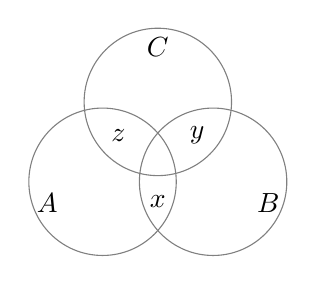
\begin{tikzpicture}[scale=0.78]
\draw[gray] (0,0.75) circle (1.2);
\draw[gray] (-0.9,-0.55) circle (1.2);
\draw[gray] (0.9,-0.55) circle (1.2);
\node at (0,1.65) {$C$};
\node at (-1.8,-0.9) {$A$};
\node at (1.8,-0.9) {$B$};
\node at (-0.64,0.20) {$z$};
\node at (0.64,0.20) {$y$};
\node at (0,-0.88) {$x$};
\end{tikzpicture}
\end{center}
\step{① 集合 $\{1,2,3,4\}$ 中的子集合有 4 个元素，所以从 $1,2,3,4$ 四个元素选 3 个有 $C_4^3=4$ 种方法，将 3 个元素进行全排列有 $P_3^3=3\times2=6$ 种，剩余的一个元素可以分别放入集合 $A$、$B$、$C$，有 3 种，所以此时共有 $3\times4\times6=72$ 种。}
\step{② 集合 $\{1,2,3,4\}$ 中的子集合有 3 个元素，满足集合 $A$、$B$、$C$ 中都只有一个元素。}
\step{所以从 $1,2,3,4$ 四个元素选 3 个有 $C_4^3=4$ 种方法，将 3 个元素进行全排列有 $P_3^3=3\times2=6$ 种，所以此时共有 $4\times6=24$ 种。}
\step{综上，共有 $72+24=96$ 个。}
\solend
\fi

\item 设 $a\in\R$，记 $f(x)=x^2+2x+a$，若关于 $x$ 的不等式 $f(f(x))<0$ 的解集为 $\varnothing$，则 $a$ 的取值范围为 \blankline[4.4em].

\ifanswer
\solbegin
\step{二次函数 $f(x)=x^2+2x+a$ 的开口向上，对称轴为 $x=-1$，所以 $f(x)_{\min}=f(-1)=a-1$，即 $f(x)$ 的值域为 $[a-1,+\infty)$.}
\step{要使不等式 $f(f(x))<0$ 的解集为空集，则 $f(f(x))\geqslant0$ 恒成立，}
\step{所以 $\begin{cases}f(a-1)\geqslant0,\\a-1\geqslant-1,\end{cases}$ 即 $\begin{cases}a^2+a-1\geqslant0,\\a\geqslant0,\end{cases}$}
\step{解得 $a\geqslant\dfrac{\sqrt5-1}{2}$，所以实数 $a$ 的取值范围为 $\left[\dfrac{\sqrt5-1}{2},+\infty\right)$.}
\solend
\fi

\end{enumerate}

\bigsec{二、选择题}

\begin{enumerate}
\setcounter{enumi}{12}

\item 已知关于 $x$ 的不等式 $2x-1>a(x-2)$ 的解集是 $\R$，则数 $a$ 的取值范围是\mbox{（\quad）}

\keepwithprev
A. $a>2$\qquad B. $a=2$

C. $a<2$\qquad D. $a$ 不存在

\ans{$B$}

\item 设 $0<a_1<a_2$，$0<b_1<b_2$，且 $a_1+a_2=b_1+b_2=1$，如果要把 $a_1b_1+a_2b_2$、$a_1b_2+a_2b_1$、$\dfrac12$ 按从小到大的顺序排列，那么排在中间的数是\mbox{（\quad）}

\keepwithprev
A. 一定是 $a_1b_1+a_2b_2$\qquad B. 一定是 $a_1b_2+a_2b_1$

C. 一定是 $\dfrac12$\qquad D. 不能确定，与 $a_1,a_2,b_1,b_2$ 的值有关

\ans{$C$}

\item “$0<a<b$”是“$a-\dfrac1a<b-\dfrac1b$”的\mbox{（\quad）}条件

\keepwithprev
A. 充分不必要\qquad B. 必要不充分

C. 充分必要\qquad D. 既不充分也不必要

\ans{$A$}

\item 在 $n$ 元集合 $S=\{a_1,a_2,\cdots,a_n\}$ 中，设 $x(S)=\dfrac{a_1+a_2+\cdots+a_n}{n}$，若 $S$ 的非空子集 $A$ 满足 $x(A)=x(S)$，则称 $A$ 是集合 $S$ 的一个“平均子集”，并记集合 $S$ 的 $k$ 个“平均子集”的个数为 $f_S(k)$. 已知集合 $S=\{1,2,3,4,5,6,7,8,9\}$，$T=\{-4,-3,-2,-1,0,1,2,3,4\}$，则下列说法错误的是\mbox{（\quad）}

\keepwithprev
A. $f_S(9)=f_T(1)$\qquad B. $f_S(8)=f_T(1)$

C. $f_S(6)=f_T(4)$\qquad D. $f_S(5)=f_T(4)$

\ans{$D$}

\ifanswer
\solbegin
\step{$X(S)=5$，将 $S$ 中的元素分成 5 组 $(1,9)$、$(2,8)$、$(3,7)$、$(4,6)$、$(5)$.}
\step{则 $f_S(1)=C_1^1=1$，$f_S(2)=C_4^1=4$，$f_S(3)=C_1^1C_4^1=4$，$f_S(4)=C_4^2=6$，$f_S(5)=C_1^1C_4^2=6$，同时 $X(T)=0$，将 $T$ 中的元素分成 5 组 $(1,-1)$、$(2,-2)$、$(3,-3)$、$(4,-4)$、$(0)$.}
\step{则 $f_T(1)=C_1^1=1$，$f_T(2)=C_4^1=4$，$f_T(3)=C_1^1C_4^1=4$，$f_T(4)=C_4^2=6$，$f_T(5)=C_1^1C_4^2=6$，$f_T(8)=C_4^4=1$，所以 $f_S(4)=f_S(5)=f_T(4)=6$，故选 D.}
\solend
\fi

\end{enumerate}

\bigsec{三、解答题}

\begin{enumerate}
\setcounter{enumi}{16}

\item 已知集合 $A=\{x\mid x^2-12x+20\leqslant0\}$，$B=\{x\mid2m<x<m+4\}$.

\begin{enumerate}[label=(\arabic*)]
\item 若 $m=3$，求 $A\cup B$；
\item 若 $A\cap B=\varnothing$，求 $m$ 的取值范围.
\end{enumerate}

\ifanswer
\solbegin
\stepm{(1)}{因为 $A=\{x\mid x^2-12x+20\leqslant0\}=\{x\mid2\leqslant x\leqslant10\}$，当 $m=3$ 时，$B=\{x\mid6<x<7\}$，所以 $A\cup B=\{x\mid2\leqslant x\leqslant10\}$.}
\stepm{(2)}{当 $m+4\leqslant2$ 时，$B$ 在 $A$ 的左侧，得 $m\leqslant-2$；当 $2m\geqslant10$ 时，得 $m\geqslant5$；当 $2m\geqslant m+4$ 时，$B=\varnothing$，得 $m\geqslant4$.}
\step{综上，$m\leqslant-2$ 或 $m\geqslant4$.}
\solend
\fi

\item 已知 $a>0$，关于 $x$ 的方程 $\dfrac1{x-2}+\dfrac1{x-1}=\dfrac{\sqrt{ax}}{x^2-3x+2}$ 有且仅有一个实数根，求实数 $a$ 的取值范围.

\ifanswer
\solbegin
\step{由题意得 $x\neq2$，$x\neq1$. 去分母整理得 $2x-3=\sqrt{ax}\geqslant0$，所以 $x\geqslant\dfrac32$，且 $x\neq2$.}
\step{两边平方整理得 $4x^2-(12+a)x+9=0$，判别式 $\Delta=a^2+24a>0$.}
\step{设方程的两个根为 $x_1$、$x_2$，则 $x_1+x_2=\dfrac{12+a}{4}$，$x_1x_2=\dfrac94$.}
\step{当 $0<a<\dfrac12$ 时，方程有一个根在 $\left(\dfrac32,2\right)$ 内，另一个根小于 $\dfrac32$，符合题意；}
\step{当 $a=\dfrac12$ 时，方程的根为 $2$、$\dfrac98$，均不符合题意；}
\step{当 $a>\dfrac12$ 时，方程有一个根大于 $2$，另一个根小于 $\dfrac32$，符合题意。}
\step{综上，实数 $a$ 的取值范围为 $\left(0,\dfrac12\right)\cup\left(\dfrac12,+\infty\right)$.}
\solend
\fi

\item 已知 $a\in\R$，关于 $x$ 的不等式 $ax^2-ax+3>0$ 恒成立.

\begin{enumerate}[label=(\arabic*)]
\item 求实数 $a$ 的取值范围；
\item 在（1）的条件下用反证法证明：三个关于 $x$ 的方程 $x^2+4ax-4a+3=0$，$x^2+(a-1)x+a^2=0$，$x^2+2ax-2a=0$ 中至少有一个方程有实数解.
\end{enumerate}

\ifanswer
\solbegin
\stepm{(1)}{当 $a=0$ 时，$3>0$ 恒成立；当 $a>0$ 时，$\Delta=a^2-12a<0$，解得 $0<a<12$；当 $a<0$ 时，不等式不恒成立。}
\step{综上，$a\in[0,12)$.}
\stepm{(2)}{假设三个方程均无实数解，则}
\step{$\begin{cases}\Delta_1=16a^2+16a-12<0,\\\Delta_2=(a-1)^2-4a^2<0,\\\Delta_3=4a^2+8a<0,\end{cases}$}
\step{解得 $-\dfrac32<a<\dfrac12$，$a<-1$ 或 $a>\dfrac13$，$-2<a<0$.}
\step{由 $a\in[0,12)$，前两个不等式得 $\dfrac13<a<\dfrac12$，第三个不等式得 $-2<a<0$，矛盾。}
\step{所以三个方程中至少有一个方程有实数解。}
\solend
\fi

% 注：原卷条件③按字面未限定 2x∈P_n；若对所有 x∈P_n 都要求 2x∈A，原卷答案 f(4)=4 与之不符。
%     2012 年江苏卷源题将其表述为相对于 P_n 的补集条件；本稿仍照录高一42原文，未替换。
\item 设集合 $P_n=\{1,2,\cdots,n\}$，$n\in\N^*$. 记 $f(n)$ 为同时满足下列条件的集合 $A$ 的个数：

① $A\subseteq P_n$；②若 $x\in A$，则 $2x\notin A$；③若 $x\notin A$，则 $2x\in A$.

\begin{enumerate}[label=(\arabic*)]
\item 求 $f(4)$；
\item 求 $f(n)$ 的解析式（用 $n$ 表示）.
\end{enumerate}

\ifanswer
\solbegin
\stepm{(1)}{当 $n=4$ 时，$P_4=\{1,2,3,4\}$，符合条件的集合 $A$ 为 $\{2\}$、$\{1,4\}$、$\{2,3\}$、$\{1,3,4\}$，故 $f(4)=4$.}
\stepm{(2)}{任取偶数 $x\in P_n$，将 $x$ 除以 2，若商仍为偶数，再除以 2，经过 $k$ 次后商必为奇数，此时商记为 $m$.}
\step{于是 $x=m\cdot2^k$，其中 $m$ 为奇数，$k\in\N^*$.}
\step{由条件得，若 $m\in A$，则 $x\in A\Longleftrightarrow k$ 为偶数；若 $m\notin A$，则 $x\in A\Longleftrightarrow k$ 为奇数。}
\step{因此每个奇数 $m\in P_n$ 是否属于 $A$ 可任意选择，且确定后其所有倍数的归属也唯一确定。}
\step{当 $n$ 为偶数时，$P_n$ 中奇数有 $\dfrac n2$ 个；当 $n$ 为奇数时，$P_n$ 中奇数有 $\dfrac{n+1}{2}$ 个。}
\step{所以 $f(n)=\begin{cases}2^{\frac n2},&n\text{ 为偶数},\\2^{\frac{n+1}{2}},&n\text{ 为奇数} .\end{cases}$}
\solend
\fi

\item 设 $S_n=\{(x_1,x_2,\cdots,x_n)\mid x_i\in\{0,1\},\ i=1,2,\cdots,n\}$（$n$ 为正整数），对任意的 $\alpha=(x_1,x_2,\cdots,x_n)$，$\beta=(y_1,y_2,\cdots,y_n)$，定义 $\alpha\cdot\beta=x_1y_1+x_2y_2+\cdots+x_ny_n$.

\begin{enumerate}[label=(\arabic*)]
\item 当 $n=3$ 时，$\alpha=(1,1,0)$，$\beta=(1,0,1)$，求 $\alpha\cdot\beta$；
\item 当 $n=3$ 时，集合 $A\subseteq S_n$，对任意 $\alpha,\beta\in A$，$\alpha\cdot\beta$ 均为偶数，求 $A$ 中元素个数的最大值；
\item 集合 $A\subseteq S_n$，对任意 $\alpha,\beta\in A$，$\alpha\neq\beta$，均有 $\alpha\cdot\beta\neq0$，求 $A$ 中元素个数的最大值.
\end{enumerate}

\ifanswer
\solbegin
\stepm{(1)}{当 $n=3$ 时，$\alpha\cdot\beta=x_1y_1+x_2y_2+x_3y_3=1\times1+1\times0+0\times1=1$.}
\stepm{(2)}{因为 $\alpha\cdot\beta=x_1y_1+x_2y_2+x_3y_3$ 均为偶数，所以结果为 $0$ 或 $2$.}
\step{当 $\alpha\cdot\beta=0$，则 $A$ 中元素个数最多有 $4$ 个；当 $\alpha\cdot\beta=2$，则 $A$ 中元素个数最多有 $1$ 个。}
\step{综上，$A$ 中元素个数的最大值为 $4$.}
\stepm{(3)}{若 $\alpha=(x_1,x_2,\cdots,x_n)\in A$，令 $\gamma=(1-x_1,1-x_2,\cdots,1-x_n)$，则 $\alpha\cdot\gamma=0$.}
\step{因为 $\alpha\cdot\beta\neq0$，$\alpha\in A$，所以 $\gamma\notin A$.}
\step{因为 $S_n$ 中有 $2^n$ 个元素，所以 $A$ 中元素个数最多有 $\dfrac{2^n}{2}=2^{n-1}$ 个。}
\step{综上，$A$ 中元素个数的最大值为 $2^{n-1}$.}
\solend
\fi

\end{enumerate}

\end{document}
"
% 紧凑版：xelatex "\def\iscompact{1}% 高一42_复旦附中_周末作业4.tex
%   —— 高一上数学“2026-2027 年复旦附中高一上周末作业 4”（试卷版/答案版）
% 试卷版：xelatex 高一42_复旦附中_周末作业4.tex
% 答案版：xelatex "\def\isanswer{1}\input{高一42_复旦附中_周末作业4.tex}"
% 紧凑版：xelatex "\def\iscompact{1}\input{高一42_复旦附中_周末作业4.tex}"
%
% 原始材料：微信公众号“魔都数学加油站”文章，作者破晓，2026-10-01 21:37 发布；
% 文章标题“27学年高一42——2026-2027年上海市复旦附中高一上周末作业4”；
% URL：https://mp.weixin.qq.com/s/nZ8aTd6K9OLS9S4-J-O7lA。
% 正文为 8 张 PNG 页（第 02、08 页 2560×3620，其余六页 4762×6735）。题目、答案及解析均据原图转录。
%
% 卷面标题行印作“2026-2027 年复旦附中高一上周末作业 4”，未印“上海市”；本稿标题照卷面，
% 年份区间按全稿惯例排 en dash。卷面未印副标题，本稿按“知识模块”口径标为“集合与常用逻辑用语、不等式”。
%
% 与原卷的排版差异：
%   ① 原文题号从第 3 题开始，本稿保留原题号；
%   ② 原卷的“一、填空题”“二、选择题”“三、解答题”改排为全稿统一的大节标题；
%   ③ 原卷填空横线统一排为 \blankline[4.4em]；选择题答案统一用 \ans{} 排在选项之后，
%      答案版与试卷版分离；原卷题目下方印出的【答案】、【解析】在答案版中排出；
%   ④ 原卷的粉色斜水印“魔都数学加油站”未录入；第 11 题解析中的三集合示意图以 TikZ 重绘。
%
% 原卷存疑处（照录原文）：
%   ① 第 5 题印出的答案为 $P>Q$，但取 $a=8,b=1$ 即得 $P=1<Q=\sqrt[3]{7}$；本稿照录；
%   ② 第 16 题解析按对称数对计数，印出 f_T(4)=C_4^2=6 并据此“故选 D”；但 T 中还可见
%      {0,1,2,-3} 这类和为 0 的四元子集，原卷的计数及选项结论疑有遗漏，本稿保留原解析和答案；
%   ③ 第 20 题的条件③印作“若 x∉A，则 2x∈A”，未明确限定 2x∈P_n；按此字面读法，f(4)
%      与【解析】列出的四个集合不符，而原题源 2012 年江苏卷明确写补集相对 P_n。
%      本稿照录原卷，不改条件，也不以源题替换；
%   ④ 第 21(2) 题题干未写 α≠β，解析结论为 4；此处照卷面题干与结论录入。
\documentclass[a4paper,11pt]{article}
\usepackage{common}

\begin{document}

\examtitlest[4]{2026--2027 年复旦附中高一上周末作业 4}{集合与常用逻辑用语、不等式}

\bigsec{一、填空题}

\begin{enumerate}
\setcounter{enumi}{2}

\item 若 $-1<x<y<2$，则 $x-y$ 的取值范围为 \blankline[4.4em].

\ifanswer
\solbegin
\step{$(-3,0)$.}
\solend
\fi

\item 已知 $c>d$，若 $ac+bd>bc+ad$，则 $a-b$ 与 $0$ 的大小关系是 \blankline[4.4em].

\ifanswer
\solbegin
\step{$a-b>0$.}
\solend
\fi

\item 已知 $a>b>0$，$P=\sqrt[3]{a}-\sqrt[3]{b}$，$Q=\sqrt[3]{a-b}$，则 $P$、$Q$ 的大小关系是 \blankline[4.4em].

\ifanswer
\solbegin
\step{$P>Q$.}
\solend
\fi

\item 对任意的实数 $x$，不等式 $x+|x-1|\geqslant m$ 恒成立，则实数 $m$ 的取值范围是 \blankline[4.4em].

\ifanswer
\solbegin
\step{令 $f(x)=x+|x-1|=\begin{cases}2x-1,&x\geqslant1,\\1,&x<1.\end{cases}$}
\step{当 $x\geqslant1$ 时，不等式变为 $2x-1\geqslant m$，显然满足题意；}
\step{当 $x<1$ 时，不等式变为 $1\geqslant m$，解得 $m\leqslant1$.}
\step{综上，$m\leqslant1$.}
\solend
\fi

\item 若“存在 $x\in\{x\mid1\leqslant x\leqslant2\}$，使得 $3x+a+1\geqslant0$”是命题，则实数 $a$ 的取值范围是 \blankline[4.4em].

\ifanswer
\solbegin
\step{由题意得 $6+a+1\geqslant0$，所以 $a\geqslant-7$.}
\solend
\fi

\item 已知关于 $x$ 的不等式 $ax-b\leqslant0$ 的解集是 $[2,+\infty)$，则关于 $x$ 的不等式
$ax^2+(3a-b)x-3b<0$ 的解集是 \blankline[4.4em].

\ifanswer
\solbegin
\step{由题意得 $a<0$，且 $\dfrac ba=2$，所以 $b=2a$.}
\step{当 $a<0$ 时，$ax^2+(3a-b)x-3b<0$ 等价于 $x^2+x-6>0$，}
\step{解得 $x\in(-\infty,-3)\cup(2,+\infty)$.}
\solend
\fi

\item 若关于 $x$ 的不等式 $(k^2+4k-5)x^2+4(1-k)x+3>0$ 恒成立，则实数 $k$ 的取值范围是 \blankline[4.4em].

\ifanswer
\solbegin
\step{当 $k=-5$ 时，不等式变为 $24x+3>0$，显然不满足题意，所以 $k\neq-5$.}
\step{当 $k=1$ 时，不等式变为 $3>0$，显然满足题意，所以 $k=1$.}
\step{当 $k^2+4k-5\neq0$ 时，有 $\begin{cases}k^2+4k-5>0,\\\Delta<0,\end{cases}$}
\step{即 $\begin{cases}k^2+4k-5>0,\\4(k-1)(k-19)<0,\end{cases}$，解得 $1<k<19$.}
\step{综上，实数 $k$ 的取值范围是 $[1,19)$.}
\solend
\fi

\item 设 $a\in\R$，集合 $A=\{x\mid x^2-ax+a\leqslant0\}$，若 $A\cap\N\neq\varnothing$，则 $a$ 的取值范围是 \blankline[4.4em].

\ifanswer
\solbegin
\step{$(-\infty,0]\cup[4,+\infty)$.}
\solend
\fi

\item 用 $|S|$ 表示集合 $S$ 中的元素的个数，设 $A$、$B$、$C$ 为集合，称 $(A,B,C)$ 为有序三元组。如果集合 $A$、$B$、$C$ 满足 $|A\cap B|=|B\cap C|=|C\cap A|=1$，且 $|A\cap B\cap C|=0$，则称有序三元组 $(A,B,C)$ 为最小交。由集合 $\{1,2,3,4\}$ 的子集构成的所有有序三元组中，最小交的有序三元组的个数为 \blankline[4.4em].

\ifanswer
\solbegin
\step{设 $A\cap B=\{x\}$，$B\cap C=\{y\}$，$C\cap A=\{z\}$，则 $x,y,z\in\{1,2,3,4\}$，且 $x,y,z$ 互不相同。}
\begin{center}
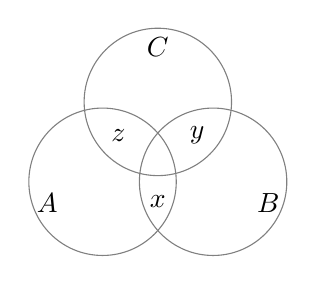
\begin{tikzpicture}[scale=0.78]
\draw[gray] (0,0.75) circle (1.2);
\draw[gray] (-0.9,-0.55) circle (1.2);
\draw[gray] (0.9,-0.55) circle (1.2);
\node at (0,1.65) {$C$};
\node at (-1.8,-0.9) {$A$};
\node at (1.8,-0.9) {$B$};
\node at (-0.64,0.20) {$z$};
\node at (0.64,0.20) {$y$};
\node at (0,-0.88) {$x$};
\end{tikzpicture}
\end{center}
\step{① 集合 $\{1,2,3,4\}$ 中的子集合有 4 个元素，所以从 $1,2,3,4$ 四个元素选 3 个有 $C_4^3=4$ 种方法，将 3 个元素进行全排列有 $P_3^3=3\times2=6$ 种，剩余的一个元素可以分别放入集合 $A$、$B$、$C$，有 3 种，所以此时共有 $3\times4\times6=72$ 种。}
\step{② 集合 $\{1,2,3,4\}$ 中的子集合有 3 个元素，满足集合 $A$、$B$、$C$ 中都只有一个元素。}
\step{所以从 $1,2,3,4$ 四个元素选 3 个有 $C_4^3=4$ 种方法，将 3 个元素进行全排列有 $P_3^3=3\times2=6$ 种，所以此时共有 $4\times6=24$ 种。}
\step{综上，共有 $72+24=96$ 个。}
\solend
\fi

\item 设 $a\in\R$，记 $f(x)=x^2+2x+a$，若关于 $x$ 的不等式 $f(f(x))<0$ 的解集为 $\varnothing$，则 $a$ 的取值范围为 \blankline[4.4em].

\ifanswer
\solbegin
\step{二次函数 $f(x)=x^2+2x+a$ 的开口向上，对称轴为 $x=-1$，所以 $f(x)_{\min}=f(-1)=a-1$，即 $f(x)$ 的值域为 $[a-1,+\infty)$.}
\step{要使不等式 $f(f(x))<0$ 的解集为空集，则 $f(f(x))\geqslant0$ 恒成立，}
\step{所以 $\begin{cases}f(a-1)\geqslant0,\\a-1\geqslant-1,\end{cases}$ 即 $\begin{cases}a^2+a-1\geqslant0,\\a\geqslant0,\end{cases}$}
\step{解得 $a\geqslant\dfrac{\sqrt5-1}{2}$，所以实数 $a$ 的取值范围为 $\left[\dfrac{\sqrt5-1}{2},+\infty\right)$.}
\solend
\fi

\end{enumerate}

\bigsec{二、选择题}

\begin{enumerate}
\setcounter{enumi}{12}

\item 已知关于 $x$ 的不等式 $2x-1>a(x-2)$ 的解集是 $\R$，则数 $a$ 的取值范围是\mbox{（\quad）}

\keepwithprev
A. $a>2$\qquad B. $a=2$

C. $a<2$\qquad D. $a$ 不存在

\ans{$B$}

\item 设 $0<a_1<a_2$，$0<b_1<b_2$，且 $a_1+a_2=b_1+b_2=1$，如果要把 $a_1b_1+a_2b_2$、$a_1b_2+a_2b_1$、$\dfrac12$ 按从小到大的顺序排列，那么排在中间的数是\mbox{（\quad）}

\keepwithprev
A. 一定是 $a_1b_1+a_2b_2$\qquad B. 一定是 $a_1b_2+a_2b_1$

C. 一定是 $\dfrac12$\qquad D. 不能确定，与 $a_1,a_2,b_1,b_2$ 的值有关

\ans{$C$}

\item “$0<a<b$”是“$a-\dfrac1a<b-\dfrac1b$”的\mbox{（\quad）}条件

\keepwithprev
A. 充分不必要\qquad B. 必要不充分

C. 充分必要\qquad D. 既不充分也不必要

\ans{$A$}

\item 在 $n$ 元集合 $S=\{a_1,a_2,\cdots,a_n\}$ 中，设 $x(S)=\dfrac{a_1+a_2+\cdots+a_n}{n}$，若 $S$ 的非空子集 $A$ 满足 $x(A)=x(S)$，则称 $A$ 是集合 $S$ 的一个“平均子集”，并记集合 $S$ 的 $k$ 个“平均子集”的个数为 $f_S(k)$. 已知集合 $S=\{1,2,3,4,5,6,7,8,9\}$，$T=\{-4,-3,-2,-1,0,1,2,3,4\}$，则下列说法错误的是\mbox{（\quad）}

\keepwithprev
A. $f_S(9)=f_T(1)$\qquad B. $f_S(8)=f_T(1)$

C. $f_S(6)=f_T(4)$\qquad D. $f_S(5)=f_T(4)$

\ans{$D$}

\ifanswer
\solbegin
\step{$X(S)=5$，将 $S$ 中的元素分成 5 组 $(1,9)$、$(2,8)$、$(3,7)$、$(4,6)$、$(5)$.}
\step{则 $f_S(1)=C_1^1=1$，$f_S(2)=C_4^1=4$，$f_S(3)=C_1^1C_4^1=4$，$f_S(4)=C_4^2=6$，$f_S(5)=C_1^1C_4^2=6$，同时 $X(T)=0$，将 $T$ 中的元素分成 5 组 $(1,-1)$、$(2,-2)$、$(3,-3)$、$(4,-4)$、$(0)$.}
\step{则 $f_T(1)=C_1^1=1$，$f_T(2)=C_4^1=4$，$f_T(3)=C_1^1C_4^1=4$，$f_T(4)=C_4^2=6$，$f_T(5)=C_1^1C_4^2=6$，$f_T(8)=C_4^4=1$，所以 $f_S(4)=f_S(5)=f_T(4)=6$，故选 D.}
\solend
\fi

\end{enumerate}

\bigsec{三、解答题}

\begin{enumerate}
\setcounter{enumi}{16}

\item 已知集合 $A=\{x\mid x^2-12x+20\leqslant0\}$，$B=\{x\mid2m<x<m+4\}$.

\begin{enumerate}[label=(\arabic*)]
\item 若 $m=3$，求 $A\cup B$；
\item 若 $A\cap B=\varnothing$，求 $m$ 的取值范围.
\end{enumerate}

\ifanswer
\solbegin
\stepm{(1)}{因为 $A=\{x\mid x^2-12x+20\leqslant0\}=\{x\mid2\leqslant x\leqslant10\}$，当 $m=3$ 时，$B=\{x\mid6<x<7\}$，所以 $A\cup B=\{x\mid2\leqslant x\leqslant10\}$.}
\stepm{(2)}{当 $m+4\leqslant2$ 时，$B$ 在 $A$ 的左侧，得 $m\leqslant-2$；当 $2m\geqslant10$ 时，得 $m\geqslant5$；当 $2m\geqslant m+4$ 时，$B=\varnothing$，得 $m\geqslant4$.}
\step{综上，$m\leqslant-2$ 或 $m\geqslant4$.}
\solend
\fi

\item 已知 $a>0$，关于 $x$ 的方程 $\dfrac1{x-2}+\dfrac1{x-1}=\dfrac{\sqrt{ax}}{x^2-3x+2}$ 有且仅有一个实数根，求实数 $a$ 的取值范围.

\ifanswer
\solbegin
\step{由题意得 $x\neq2$，$x\neq1$. 去分母整理得 $2x-3=\sqrt{ax}\geqslant0$，所以 $x\geqslant\dfrac32$，且 $x\neq2$.}
\step{两边平方整理得 $4x^2-(12+a)x+9=0$，判别式 $\Delta=a^2+24a>0$.}
\step{设方程的两个根为 $x_1$、$x_2$，则 $x_1+x_2=\dfrac{12+a}{4}$，$x_1x_2=\dfrac94$.}
\step{当 $0<a<\dfrac12$ 时，方程有一个根在 $\left(\dfrac32,2\right)$ 内，另一个根小于 $\dfrac32$，符合题意；}
\step{当 $a=\dfrac12$ 时，方程的根为 $2$、$\dfrac98$，均不符合题意；}
\step{当 $a>\dfrac12$ 时，方程有一个根大于 $2$，另一个根小于 $\dfrac32$，符合题意。}
\step{综上，实数 $a$ 的取值范围为 $\left(0,\dfrac12\right)\cup\left(\dfrac12,+\infty\right)$.}
\solend
\fi

\item 已知 $a\in\R$，关于 $x$ 的不等式 $ax^2-ax+3>0$ 恒成立.

\begin{enumerate}[label=(\arabic*)]
\item 求实数 $a$ 的取值范围；
\item 在（1）的条件下用反证法证明：三个关于 $x$ 的方程 $x^2+4ax-4a+3=0$，$x^2+(a-1)x+a^2=0$，$x^2+2ax-2a=0$ 中至少有一个方程有实数解.
\end{enumerate}

\ifanswer
\solbegin
\stepm{(1)}{当 $a=0$ 时，$3>0$ 恒成立；当 $a>0$ 时，$\Delta=a^2-12a<0$，解得 $0<a<12$；当 $a<0$ 时，不等式不恒成立。}
\step{综上，$a\in[0,12)$.}
\stepm{(2)}{假设三个方程均无实数解，则}
\step{$\begin{cases}\Delta_1=16a^2+16a-12<0,\\\Delta_2=(a-1)^2-4a^2<0,\\\Delta_3=4a^2+8a<0,\end{cases}$}
\step{解得 $-\dfrac32<a<\dfrac12$，$a<-1$ 或 $a>\dfrac13$，$-2<a<0$.}
\step{由 $a\in[0,12)$，前两个不等式得 $\dfrac13<a<\dfrac12$，第三个不等式得 $-2<a<0$，矛盾。}
\step{所以三个方程中至少有一个方程有实数解。}
\solend
\fi

% 注：原卷条件③按字面未限定 2x∈P_n；若对所有 x∈P_n 都要求 2x∈A，原卷答案 f(4)=4 与之不符。
%     2012 年江苏卷源题将其表述为相对于 P_n 的补集条件；本稿仍照录高一42原文，未替换。
\item 设集合 $P_n=\{1,2,\cdots,n\}$，$n\in\N^*$. 记 $f(n)$ 为同时满足下列条件的集合 $A$ 的个数：

① $A\subseteq P_n$；②若 $x\in A$，则 $2x\notin A$；③若 $x\notin A$，则 $2x\in A$.

\begin{enumerate}[label=(\arabic*)]
\item 求 $f(4)$；
\item 求 $f(n)$ 的解析式（用 $n$ 表示）.
\end{enumerate}

\ifanswer
\solbegin
\stepm{(1)}{当 $n=4$ 时，$P_4=\{1,2,3,4\}$，符合条件的集合 $A$ 为 $\{2\}$、$\{1,4\}$、$\{2,3\}$、$\{1,3,4\}$，故 $f(4)=4$.}
\stepm{(2)}{任取偶数 $x\in P_n$，将 $x$ 除以 2，若商仍为偶数，再除以 2，经过 $k$ 次后商必为奇数，此时商记为 $m$.}
\step{于是 $x=m\cdot2^k$，其中 $m$ 为奇数，$k\in\N^*$.}
\step{由条件得，若 $m\in A$，则 $x\in A\Longleftrightarrow k$ 为偶数；若 $m\notin A$，则 $x\in A\Longleftrightarrow k$ 为奇数。}
\step{因此每个奇数 $m\in P_n$ 是否属于 $A$ 可任意选择，且确定后其所有倍数的归属也唯一确定。}
\step{当 $n$ 为偶数时，$P_n$ 中奇数有 $\dfrac n2$ 个；当 $n$ 为奇数时，$P_n$ 中奇数有 $\dfrac{n+1}{2}$ 个。}
\step{所以 $f(n)=\begin{cases}2^{\frac n2},&n\text{ 为偶数},\\2^{\frac{n+1}{2}},&n\text{ 为奇数} .\end{cases}$}
\solend
\fi

\item 设 $S_n=\{(x_1,x_2,\cdots,x_n)\mid x_i\in\{0,1\},\ i=1,2,\cdots,n\}$（$n$ 为正整数），对任意的 $\alpha=(x_1,x_2,\cdots,x_n)$，$\beta=(y_1,y_2,\cdots,y_n)$，定义 $\alpha\cdot\beta=x_1y_1+x_2y_2+\cdots+x_ny_n$.

\begin{enumerate}[label=(\arabic*)]
\item 当 $n=3$ 时，$\alpha=(1,1,0)$，$\beta=(1,0,1)$，求 $\alpha\cdot\beta$；
\item 当 $n=3$ 时，集合 $A\subseteq S_n$，对任意 $\alpha,\beta\in A$，$\alpha\cdot\beta$ 均为偶数，求 $A$ 中元素个数的最大值；
\item 集合 $A\subseteq S_n$，对任意 $\alpha,\beta\in A$，$\alpha\neq\beta$，均有 $\alpha\cdot\beta\neq0$，求 $A$ 中元素个数的最大值.
\end{enumerate}

\ifanswer
\solbegin
\stepm{(1)}{当 $n=3$ 时，$\alpha\cdot\beta=x_1y_1+x_2y_2+x_3y_3=1\times1+1\times0+0\times1=1$.}
\stepm{(2)}{因为 $\alpha\cdot\beta=x_1y_1+x_2y_2+x_3y_3$ 均为偶数，所以结果为 $0$ 或 $2$.}
\step{当 $\alpha\cdot\beta=0$，则 $A$ 中元素个数最多有 $4$ 个；当 $\alpha\cdot\beta=2$，则 $A$ 中元素个数最多有 $1$ 个。}
\step{综上，$A$ 中元素个数的最大值为 $4$.}
\stepm{(3)}{若 $\alpha=(x_1,x_2,\cdots,x_n)\in A$，令 $\gamma=(1-x_1,1-x_2,\cdots,1-x_n)$，则 $\alpha\cdot\gamma=0$.}
\step{因为 $\alpha\cdot\beta\neq0$，$\alpha\in A$，所以 $\gamma\notin A$.}
\step{因为 $S_n$ 中有 $2^n$ 个元素，所以 $A$ 中元素个数最多有 $\dfrac{2^n}{2}=2^{n-1}$ 个。}
\step{综上，$A$ 中元素个数的最大值为 $2^{n-1}$.}
\solend
\fi

\end{enumerate}

\end{document}
"
%
% 原始材料：微信公众号“魔都数学加油站”文章，作者破晓，2026-10-01 21:37 发布；
% 文章标题“27学年高一42——2026-2027年上海市复旦附中高一上周末作业4”；
% URL：https://mp.weixin.qq.com/s/nZ8aTd6K9OLS9S4-J-O7lA。
% 正文为 8 张 PNG 页（第 02、08 页 2560×3620，其余六页 4762×6735）。题目、答案及解析均据原图转录。
%
% 卷面标题行印作“2026-2027 年复旦附中高一上周末作业 4”，未印“上海市”；本稿标题照卷面，
% 年份区间按全稿惯例排 en dash。卷面未印副标题，本稿按“知识模块”口径标为“集合与常用逻辑用语、不等式”。
%
% 与原卷的排版差异：
%   ① 原文题号从第 3 题开始，本稿保留原题号；
%   ② 原卷的“一、填空题”“二、选择题”“三、解答题”改排为全稿统一的大节标题；
%   ③ 原卷填空横线统一排为 \blankline[4.4em]；选择题答案统一用 \ans{} 排在选项之后，
%      答案版与试卷版分离；原卷题目下方印出的【答案】、【解析】在答案版中排出；
%   ④ 原卷的粉色斜水印“魔都数学加油站”未录入；第 11 题解析中的三集合示意图以 TikZ 重绘。
%
% 原卷存疑处（照录原文）：
%   ① 第 5 题印出的答案为 $P>Q$，但取 $a=8,b=1$ 即得 $P=1<Q=\sqrt[3]{7}$；本稿照录；
%   ② 第 16 题解析按对称数对计数，印出 f_T(4)=C_4^2=6 并据此“故选 D”；但 T 中还可见
%      {0,1,2,-3} 这类和为 0 的四元子集，原卷的计数及选项结论疑有遗漏，本稿保留原解析和答案；
%   ③ 第 20 题的条件③印作“若 x∉A，则 2x∈A”，未明确限定 2x∈P_n；按此字面读法，f(4)
%      与【解析】列出的四个集合不符，而原题源 2012 年江苏卷明确写补集相对 P_n。
%      本稿照录原卷，不改条件，也不以源题替换；
%   ④ 第 21(2) 题题干未写 α≠β，解析结论为 4；此处照卷面题干与结论录入。
\documentclass[a4paper,11pt]{article}
\usepackage{common}

\begin{document}

\examtitlest[4]{2026--2027 年复旦附中高一上周末作业 4}{集合与常用逻辑用语、不等式}

\bigsec{一、填空题}

\begin{enumerate}
\setcounter{enumi}{2}

\item 若 $-1<x<y<2$，则 $x-y$ 的取值范围为 \blankline[4.4em].

\ifanswer
\solbegin
\step{$(-3,0)$.}
\solend
\fi

\item 已知 $c>d$，若 $ac+bd>bc+ad$，则 $a-b$ 与 $0$ 的大小关系是 \blankline[4.4em].

\ifanswer
\solbegin
\step{$a-b>0$.}
\solend
\fi

\item 已知 $a>b>0$，$P=\sqrt[3]{a}-\sqrt[3]{b}$，$Q=\sqrt[3]{a-b}$，则 $P$、$Q$ 的大小关系是 \blankline[4.4em].

\ifanswer
\solbegin
\step{$P>Q$.}
\solend
\fi

\item 对任意的实数 $x$，不等式 $x+|x-1|\geqslant m$ 恒成立，则实数 $m$ 的取值范围是 \blankline[4.4em].

\ifanswer
\solbegin
\step{令 $f(x)=x+|x-1|=\begin{cases}2x-1,&x\geqslant1,\\1,&x<1.\end{cases}$}
\step{当 $x\geqslant1$ 时，不等式变为 $2x-1\geqslant m$，显然满足题意；}
\step{当 $x<1$ 时，不等式变为 $1\geqslant m$，解得 $m\leqslant1$.}
\step{综上，$m\leqslant1$.}
\solend
\fi

\item 若“存在 $x\in\{x\mid1\leqslant x\leqslant2\}$，使得 $3x+a+1\geqslant0$”是命题，则实数 $a$ 的取值范围是 \blankline[4.4em].

\ifanswer
\solbegin
\step{由题意得 $6+a+1\geqslant0$，所以 $a\geqslant-7$.}
\solend
\fi

\item 已知关于 $x$ 的不等式 $ax-b\leqslant0$ 的解集是 $[2,+\infty)$，则关于 $x$ 的不等式
$ax^2+(3a-b)x-3b<0$ 的解集是 \blankline[4.4em].

\ifanswer
\solbegin
\step{由题意得 $a<0$，且 $\dfrac ba=2$，所以 $b=2a$.}
\step{当 $a<0$ 时，$ax^2+(3a-b)x-3b<0$ 等价于 $x^2+x-6>0$，}
\step{解得 $x\in(-\infty,-3)\cup(2,+\infty)$.}
\solend
\fi

\item 若关于 $x$ 的不等式 $(k^2+4k-5)x^2+4(1-k)x+3>0$ 恒成立，则实数 $k$ 的取值范围是 \blankline[4.4em].

\ifanswer
\solbegin
\step{当 $k=-5$ 时，不等式变为 $24x+3>0$，显然不满足题意，所以 $k\neq-5$.}
\step{当 $k=1$ 时，不等式变为 $3>0$，显然满足题意，所以 $k=1$.}
\step{当 $k^2+4k-5\neq0$ 时，有 $\begin{cases}k^2+4k-5>0,\\\Delta<0,\end{cases}$}
\step{即 $\begin{cases}k^2+4k-5>0,\\4(k-1)(k-19)<0,\end{cases}$，解得 $1<k<19$.}
\step{综上，实数 $k$ 的取值范围是 $[1,19)$.}
\solend
\fi

\item 设 $a\in\R$，集合 $A=\{x\mid x^2-ax+a\leqslant0\}$，若 $A\cap\N\neq\varnothing$，则 $a$ 的取值范围是 \blankline[4.4em].

\ifanswer
\solbegin
\step{$(-\infty,0]\cup[4,+\infty)$.}
\solend
\fi

\item 用 $|S|$ 表示集合 $S$ 中的元素的个数，设 $A$、$B$、$C$ 为集合，称 $(A,B,C)$ 为有序三元组。如果集合 $A$、$B$、$C$ 满足 $|A\cap B|=|B\cap C|=|C\cap A|=1$，且 $|A\cap B\cap C|=0$，则称有序三元组 $(A,B,C)$ 为最小交。由集合 $\{1,2,3,4\}$ 的子集构成的所有有序三元组中，最小交的有序三元组的个数为 \blankline[4.4em].

\ifanswer
\solbegin
\step{设 $A\cap B=\{x\}$，$B\cap C=\{y\}$，$C\cap A=\{z\}$，则 $x,y,z\in\{1,2,3,4\}$，且 $x,y,z$ 互不相同。}
\begin{center}
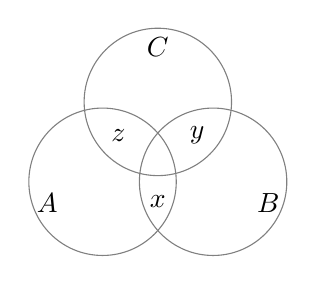
\begin{tikzpicture}[scale=0.78]
\draw[gray] (0,0.75) circle (1.2);
\draw[gray] (-0.9,-0.55) circle (1.2);
\draw[gray] (0.9,-0.55) circle (1.2);
\node at (0,1.65) {$C$};
\node at (-1.8,-0.9) {$A$};
\node at (1.8,-0.9) {$B$};
\node at (-0.64,0.20) {$z$};
\node at (0.64,0.20) {$y$};
\node at (0,-0.88) {$x$};
\end{tikzpicture}
\end{center}
\step{① 集合 $\{1,2,3,4\}$ 中的子集合有 4 个元素，所以从 $1,2,3,4$ 四个元素选 3 个有 $C_4^3=4$ 种方法，将 3 个元素进行全排列有 $P_3^3=3\times2=6$ 种，剩余的一个元素可以分别放入集合 $A$、$B$、$C$，有 3 种，所以此时共有 $3\times4\times6=72$ 种。}
\step{② 集合 $\{1,2,3,4\}$ 中的子集合有 3 个元素，满足集合 $A$、$B$、$C$ 中都只有一个元素。}
\step{所以从 $1,2,3,4$ 四个元素选 3 个有 $C_4^3=4$ 种方法，将 3 个元素进行全排列有 $P_3^3=3\times2=6$ 种，所以此时共有 $4\times6=24$ 种。}
\step{综上，共有 $72+24=96$ 个。}
\solend
\fi

\item 设 $a\in\R$，记 $f(x)=x^2+2x+a$，若关于 $x$ 的不等式 $f(f(x))<0$ 的解集为 $\varnothing$，则 $a$ 的取值范围为 \blankline[4.4em].

\ifanswer
\solbegin
\step{二次函数 $f(x)=x^2+2x+a$ 的开口向上，对称轴为 $x=-1$，所以 $f(x)_{\min}=f(-1)=a-1$，即 $f(x)$ 的值域为 $[a-1,+\infty)$.}
\step{要使不等式 $f(f(x))<0$ 的解集为空集，则 $f(f(x))\geqslant0$ 恒成立，}
\step{所以 $\begin{cases}f(a-1)\geqslant0,\\a-1\geqslant-1,\end{cases}$ 即 $\begin{cases}a^2+a-1\geqslant0,\\a\geqslant0,\end{cases}$}
\step{解得 $a\geqslant\dfrac{\sqrt5-1}{2}$，所以实数 $a$ 的取值范围为 $\left[\dfrac{\sqrt5-1}{2},+\infty\right)$.}
\solend
\fi

\end{enumerate}

\bigsec{二、选择题}

\begin{enumerate}
\setcounter{enumi}{12}

\item 已知关于 $x$ 的不等式 $2x-1>a(x-2)$ 的解集是 $\R$，则数 $a$ 的取值范围是\mbox{（\quad）}

\keepwithprev
A. $a>2$\qquad B. $a=2$

C. $a<2$\qquad D. $a$ 不存在

\ans{$B$}

\item 设 $0<a_1<a_2$，$0<b_1<b_2$，且 $a_1+a_2=b_1+b_2=1$，如果要把 $a_1b_1+a_2b_2$、$a_1b_2+a_2b_1$、$\dfrac12$ 按从小到大的顺序排列，那么排在中间的数是\mbox{（\quad）}

\keepwithprev
A. 一定是 $a_1b_1+a_2b_2$\qquad B. 一定是 $a_1b_2+a_2b_1$

C. 一定是 $\dfrac12$\qquad D. 不能确定，与 $a_1,a_2,b_1,b_2$ 的值有关

\ans{$C$}

\item “$0<a<b$”是“$a-\dfrac1a<b-\dfrac1b$”的\mbox{（\quad）}条件

\keepwithprev
A. 充分不必要\qquad B. 必要不充分

C. 充分必要\qquad D. 既不充分也不必要

\ans{$A$}

\item 在 $n$ 元集合 $S=\{a_1,a_2,\cdots,a_n\}$ 中，设 $x(S)=\dfrac{a_1+a_2+\cdots+a_n}{n}$，若 $S$ 的非空子集 $A$ 满足 $x(A)=x(S)$，则称 $A$ 是集合 $S$ 的一个“平均子集”，并记集合 $S$ 的 $k$ 个“平均子集”的个数为 $f_S(k)$. 已知集合 $S=\{1,2,3,4,5,6,7,8,9\}$，$T=\{-4,-3,-2,-1,0,1,2,3,4\}$，则下列说法错误的是\mbox{（\quad）}

\keepwithprev
A. $f_S(9)=f_T(1)$\qquad B. $f_S(8)=f_T(1)$

C. $f_S(6)=f_T(4)$\qquad D. $f_S(5)=f_T(4)$

\ans{$D$}

\ifanswer
\solbegin
\step{$X(S)=5$，将 $S$ 中的元素分成 5 组 $(1,9)$、$(2,8)$、$(3,7)$、$(4,6)$、$(5)$.}
\step{则 $f_S(1)=C_1^1=1$，$f_S(2)=C_4^1=4$，$f_S(3)=C_1^1C_4^1=4$，$f_S(4)=C_4^2=6$，$f_S(5)=C_1^1C_4^2=6$，同时 $X(T)=0$，将 $T$ 中的元素分成 5 组 $(1,-1)$、$(2,-2)$、$(3,-3)$、$(4,-4)$、$(0)$.}
\step{则 $f_T(1)=C_1^1=1$，$f_T(2)=C_4^1=4$，$f_T(3)=C_1^1C_4^1=4$，$f_T(4)=C_4^2=6$，$f_T(5)=C_1^1C_4^2=6$，$f_T(8)=C_4^4=1$，所以 $f_S(4)=f_S(5)=f_T(4)=6$，故选 D.}
\solend
\fi

\end{enumerate}

\bigsec{三、解答题}

\begin{enumerate}
\setcounter{enumi}{16}

\item 已知集合 $A=\{x\mid x^2-12x+20\leqslant0\}$，$B=\{x\mid2m<x<m+4\}$.

\begin{enumerate}[label=(\arabic*)]
\item 若 $m=3$，求 $A\cup B$；
\item 若 $A\cap B=\varnothing$，求 $m$ 的取值范围.
\end{enumerate}

\ifanswer
\solbegin
\stepm{(1)}{因为 $A=\{x\mid x^2-12x+20\leqslant0\}=\{x\mid2\leqslant x\leqslant10\}$，当 $m=3$ 时，$B=\{x\mid6<x<7\}$，所以 $A\cup B=\{x\mid2\leqslant x\leqslant10\}$.}
\stepm{(2)}{当 $m+4\leqslant2$ 时，$B$ 在 $A$ 的左侧，得 $m\leqslant-2$；当 $2m\geqslant10$ 时，得 $m\geqslant5$；当 $2m\geqslant m+4$ 时，$B=\varnothing$，得 $m\geqslant4$.}
\step{综上，$m\leqslant-2$ 或 $m\geqslant4$.}
\solend
\fi

\item 已知 $a>0$，关于 $x$ 的方程 $\dfrac1{x-2}+\dfrac1{x-1}=\dfrac{\sqrt{ax}}{x^2-3x+2}$ 有且仅有一个实数根，求实数 $a$ 的取值范围.

\ifanswer
\solbegin
\step{由题意得 $x\neq2$，$x\neq1$. 去分母整理得 $2x-3=\sqrt{ax}\geqslant0$，所以 $x\geqslant\dfrac32$，且 $x\neq2$.}
\step{两边平方整理得 $4x^2-(12+a)x+9=0$，判别式 $\Delta=a^2+24a>0$.}
\step{设方程的两个根为 $x_1$、$x_2$，则 $x_1+x_2=\dfrac{12+a}{4}$，$x_1x_2=\dfrac94$.}
\step{当 $0<a<\dfrac12$ 时，方程有一个根在 $\left(\dfrac32,2\right)$ 内，另一个根小于 $\dfrac32$，符合题意；}
\step{当 $a=\dfrac12$ 时，方程的根为 $2$、$\dfrac98$，均不符合题意；}
\step{当 $a>\dfrac12$ 时，方程有一个根大于 $2$，另一个根小于 $\dfrac32$，符合题意。}
\step{综上，实数 $a$ 的取值范围为 $\left(0,\dfrac12\right)\cup\left(\dfrac12,+\infty\right)$.}
\solend
\fi

\item 已知 $a\in\R$，关于 $x$ 的不等式 $ax^2-ax+3>0$ 恒成立.

\begin{enumerate}[label=(\arabic*)]
\item 求实数 $a$ 的取值范围；
\item 在（1）的条件下用反证法证明：三个关于 $x$ 的方程 $x^2+4ax-4a+3=0$，$x^2+(a-1)x+a^2=0$，$x^2+2ax-2a=0$ 中至少有一个方程有实数解.
\end{enumerate}

\ifanswer
\solbegin
\stepm{(1)}{当 $a=0$ 时，$3>0$ 恒成立；当 $a>0$ 时，$\Delta=a^2-12a<0$，解得 $0<a<12$；当 $a<0$ 时，不等式不恒成立。}
\step{综上，$a\in[0,12)$.}
\stepm{(2)}{假设三个方程均无实数解，则}
\step{$\begin{cases}\Delta_1=16a^2+16a-12<0,\\\Delta_2=(a-1)^2-4a^2<0,\\\Delta_3=4a^2+8a<0,\end{cases}$}
\step{解得 $-\dfrac32<a<\dfrac12$，$a<-1$ 或 $a>\dfrac13$，$-2<a<0$.}
\step{由 $a\in[0,12)$，前两个不等式得 $\dfrac13<a<\dfrac12$，第三个不等式得 $-2<a<0$，矛盾。}
\step{所以三个方程中至少有一个方程有实数解。}
\solend
\fi

% 注：原卷条件③按字面未限定 2x∈P_n；若对所有 x∈P_n 都要求 2x∈A，原卷答案 f(4)=4 与之不符。
%     2012 年江苏卷源题将其表述为相对于 P_n 的补集条件；本稿仍照录高一42原文，未替换。
\item 设集合 $P_n=\{1,2,\cdots,n\}$，$n\in\N^*$. 记 $f(n)$ 为同时满足下列条件的集合 $A$ 的个数：

① $A\subseteq P_n$；②若 $x\in A$，则 $2x\notin A$；③若 $x\notin A$，则 $2x\in A$.

\begin{enumerate}[label=(\arabic*)]
\item 求 $f(4)$；
\item 求 $f(n)$ 的解析式（用 $n$ 表示）.
\end{enumerate}

\ifanswer
\solbegin
\stepm{(1)}{当 $n=4$ 时，$P_4=\{1,2,3,4\}$，符合条件的集合 $A$ 为 $\{2\}$、$\{1,4\}$、$\{2,3\}$、$\{1,3,4\}$，故 $f(4)=4$.}
\stepm{(2)}{任取偶数 $x\in P_n$，将 $x$ 除以 2，若商仍为偶数，再除以 2，经过 $k$ 次后商必为奇数，此时商记为 $m$.}
\step{于是 $x=m\cdot2^k$，其中 $m$ 为奇数，$k\in\N^*$.}
\step{由条件得，若 $m\in A$，则 $x\in A\Longleftrightarrow k$ 为偶数；若 $m\notin A$，则 $x\in A\Longleftrightarrow k$ 为奇数。}
\step{因此每个奇数 $m\in P_n$ 是否属于 $A$ 可任意选择，且确定后其所有倍数的归属也唯一确定。}
\step{当 $n$ 为偶数时，$P_n$ 中奇数有 $\dfrac n2$ 个；当 $n$ 为奇数时，$P_n$ 中奇数有 $\dfrac{n+1}{2}$ 个。}
\step{所以 $f(n)=\begin{cases}2^{\frac n2},&n\text{ 为偶数},\\2^{\frac{n+1}{2}},&n\text{ 为奇数} .\end{cases}$}
\solend
\fi

\item 设 $S_n=\{(x_1,x_2,\cdots,x_n)\mid x_i\in\{0,1\},\ i=1,2,\cdots,n\}$（$n$ 为正整数），对任意的 $\alpha=(x_1,x_2,\cdots,x_n)$，$\beta=(y_1,y_2,\cdots,y_n)$，定义 $\alpha\cdot\beta=x_1y_1+x_2y_2+\cdots+x_ny_n$.

\begin{enumerate}[label=(\arabic*)]
\item 当 $n=3$ 时，$\alpha=(1,1,0)$，$\beta=(1,0,1)$，求 $\alpha\cdot\beta$；
\item 当 $n=3$ 时，集合 $A\subseteq S_n$，对任意 $\alpha,\beta\in A$，$\alpha\cdot\beta$ 均为偶数，求 $A$ 中元素个数的最大值；
\item 集合 $A\subseteq S_n$，对任意 $\alpha,\beta\in A$，$\alpha\neq\beta$，均有 $\alpha\cdot\beta\neq0$，求 $A$ 中元素个数的最大值.
\end{enumerate}

\ifanswer
\solbegin
\stepm{(1)}{当 $n=3$ 时，$\alpha\cdot\beta=x_1y_1+x_2y_2+x_3y_3=1\times1+1\times0+0\times1=1$.}
\stepm{(2)}{因为 $\alpha\cdot\beta=x_1y_1+x_2y_2+x_3y_3$ 均为偶数，所以结果为 $0$ 或 $2$.}
\step{当 $\alpha\cdot\beta=0$，则 $A$ 中元素个数最多有 $4$ 个；当 $\alpha\cdot\beta=2$，则 $A$ 中元素个数最多有 $1$ 个。}
\step{综上，$A$ 中元素个数的最大值为 $4$.}
\stepm{(3)}{若 $\alpha=(x_1,x_2,\cdots,x_n)\in A$，令 $\gamma=(1-x_1,1-x_2,\cdots,1-x_n)$，则 $\alpha\cdot\gamma=0$.}
\step{因为 $\alpha\cdot\beta\neq0$，$\alpha\in A$，所以 $\gamma\notin A$.}
\step{因为 $S_n$ 中有 $2^n$ 个元素，所以 $A$ 中元素个数最多有 $\dfrac{2^n}{2}=2^{n-1}$ 个。}
\step{综上，$A$ 中元素个数的最大值为 $2^{n-1}$.}
\solend
\fi

\end{enumerate}

\end{document}
"
%
% 原始材料：微信公众号“魔都数学加油站”文章，作者破晓，2026-10-01 21:37 发布；
% 文章标题“27学年高一42——2026-2027年上海市复旦附中高一上周末作业4”；
% URL：https://mp.weixin.qq.com/s/nZ8aTd6K9OLS9S4-J-O7lA。
% 正文为 8 张 PNG 页（第 02、08 页 2560×3620，其余六页 4762×6735）。题目、答案及解析均据原图转录。
%
% 卷面标题行印作“2026-2027 年复旦附中高一上周末作业 4”，未印“上海市”；本稿标题照卷面，
% 年份区间按全稿惯例排 en dash。卷面未印副标题，本稿按“知识模块”口径标为“集合与常用逻辑用语、不等式”。
%
% 与原卷的排版差异：
%   ① 原文题号从第 3 题开始，本稿保留原题号；
%   ② 原卷的“一、填空题”“二、选择题”“三、解答题”改排为全稿统一的大节标题；
%   ③ 原卷填空横线统一排为 \blankline[4.4em]；选择题答案统一用 \ans{} 排在选项之后，
%      答案版与试卷版分离；原卷题目下方印出的【答案】、【解析】在答案版中排出；
%   ④ 原卷的粉色斜水印“魔都数学加油站”未录入；第 11 题解析中的三集合示意图以 TikZ 重绘。
%
% 原卷存疑处（照录原文）：
%   ① 第 5 题印出的答案为 $P>Q$，但取 $a=8,b=1$ 即得 $P=1<Q=\sqrt[3]{7}$；本稿照录；
%   ② 第 16 题解析按对称数对计数，印出 f_T(4)=C_4^2=6 并据此“故选 D”；但 T 中还可见
%      {0,1,2,-3} 这类和为 0 的四元子集，原卷的计数及选项结论疑有遗漏，本稿保留原解析和答案；
%   ③ 第 20 题的条件③印作“若 x∉A，则 2x∈A”，未明确限定 2x∈P_n；按此字面读法，f(4)
%      与【解析】列出的四个集合不符，而原题源 2012 年江苏卷明确写补集相对 P_n。
%      本稿照录原卷，不改条件，也不以源题替换；
%   ④ 第 21(2) 题题干未写 α≠β，解析结论为 4；此处照卷面题干与结论录入。
\documentclass[a4paper,11pt]{article}
\usepackage{common}

\begin{document}

\examtitlest[4]{2026--2027 年复旦附中高一上周末作业 4}{集合与常用逻辑用语、不等式}

\bigsec{一、填空题}

\begin{enumerate}
\setcounter{enumi}{2}

\item 若 $-1<x<y<2$，则 $x-y$ 的取值范围为 \blankline[4.4em].

\ifanswer
\solbegin
\step{$(-3,0)$.}
\solend
\fi

\item 已知 $c>d$，若 $ac+bd>bc+ad$，则 $a-b$ 与 $0$ 的大小关系是 \blankline[4.4em].

\ifanswer
\solbegin
\step{$a-b>0$.}
\solend
\fi

\item 已知 $a>b>0$，$P=\sqrt[3]{a}-\sqrt[3]{b}$，$Q=\sqrt[3]{a-b}$，则 $P$、$Q$ 的大小关系是 \blankline[4.4em].

\ifanswer
\solbegin
\step{$P>Q$.}
\solend
\fi

\item 对任意的实数 $x$，不等式 $x+|x-1|\geqslant m$ 恒成立，则实数 $m$ 的取值范围是 \blankline[4.4em].

\ifanswer
\solbegin
\step{令 $f(x)=x+|x-1|=\begin{cases}2x-1,&x\geqslant1,\\1,&x<1.\end{cases}$}
\step{当 $x\geqslant1$ 时，不等式变为 $2x-1\geqslant m$，显然满足题意；}
\step{当 $x<1$ 时，不等式变为 $1\geqslant m$，解得 $m\leqslant1$.}
\step{综上，$m\leqslant1$.}
\solend
\fi

\item 若“存在 $x\in\{x\mid1\leqslant x\leqslant2\}$，使得 $3x+a+1\geqslant0$”是命题，则实数 $a$ 的取值范围是 \blankline[4.4em].

\ifanswer
\solbegin
\step{由题意得 $6+a+1\geqslant0$，所以 $a\geqslant-7$.}
\solend
\fi

\item 已知关于 $x$ 的不等式 $ax-b\leqslant0$ 的解集是 $[2,+\infty)$，则关于 $x$ 的不等式
$ax^2+(3a-b)x-3b<0$ 的解集是 \blankline[4.4em].

\ifanswer
\solbegin
\step{由题意得 $a<0$，且 $\dfrac ba=2$，所以 $b=2a$.}
\step{当 $a<0$ 时，$ax^2+(3a-b)x-3b<0$ 等价于 $x^2+x-6>0$，}
\step{解得 $x\in(-\infty,-3)\cup(2,+\infty)$.}
\solend
\fi

\item 若关于 $x$ 的不等式 $(k^2+4k-5)x^2+4(1-k)x+3>0$ 恒成立，则实数 $k$ 的取值范围是 \blankline[4.4em].

\ifanswer
\solbegin
\step{当 $k=-5$ 时，不等式变为 $24x+3>0$，显然不满足题意，所以 $k\neq-5$.}
\step{当 $k=1$ 时，不等式变为 $3>0$，显然满足题意，所以 $k=1$.}
\step{当 $k^2+4k-5\neq0$ 时，有 $\begin{cases}k^2+4k-5>0,\\\Delta<0,\end{cases}$}
\step{即 $\begin{cases}k^2+4k-5>0,\\4(k-1)(k-19)<0,\end{cases}$，解得 $1<k<19$.}
\step{综上，实数 $k$ 的取值范围是 $[1,19)$.}
\solend
\fi

\item 设 $a\in\R$，集合 $A=\{x\mid x^2-ax+a\leqslant0\}$，若 $A\cap\N\neq\varnothing$，则 $a$ 的取值范围是 \blankline[4.4em].

\ifanswer
\solbegin
\step{$(-\infty,0]\cup[4,+\infty)$.}
\solend
\fi

\item 用 $|S|$ 表示集合 $S$ 中的元素的个数，设 $A$、$B$、$C$ 为集合，称 $(A,B,C)$ 为有序三元组。如果集合 $A$、$B$、$C$ 满足 $|A\cap B|=|B\cap C|=|C\cap A|=1$，且 $|A\cap B\cap C|=0$，则称有序三元组 $(A,B,C)$ 为最小交。由集合 $\{1,2,3,4\}$ 的子集构成的所有有序三元组中，最小交的有序三元组的个数为 \blankline[4.4em].

\ifanswer
\solbegin
\step{设 $A\cap B=\{x\}$，$B\cap C=\{y\}$，$C\cap A=\{z\}$，则 $x,y,z\in\{1,2,3,4\}$，且 $x,y,z$ 互不相同。}
\begin{center}
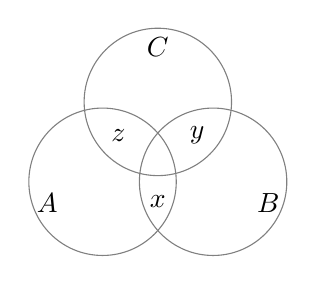
\begin{tikzpicture}[scale=0.78]
\draw[gray] (0,0.75) circle (1.2);
\draw[gray] (-0.9,-0.55) circle (1.2);
\draw[gray] (0.9,-0.55) circle (1.2);
\node at (0,1.65) {$C$};
\node at (-1.8,-0.9) {$A$};
\node at (1.8,-0.9) {$B$};
\node at (-0.64,0.20) {$z$};
\node at (0.64,0.20) {$y$};
\node at (0,-0.88) {$x$};
\end{tikzpicture}
\end{center}
\step{① 集合 $\{1,2,3,4\}$ 中的子集合有 4 个元素，所以从 $1,2,3,4$ 四个元素选 3 个有 $C_4^3=4$ 种方法，将 3 个元素进行全排列有 $P_3^3=3\times2=6$ 种，剩余的一个元素可以分别放入集合 $A$、$B$、$C$，有 3 种，所以此时共有 $3\times4\times6=72$ 种。}
\step{② 集合 $\{1,2,3,4\}$ 中的子集合有 3 个元素，满足集合 $A$、$B$、$C$ 中都只有一个元素。}
\step{所以从 $1,2,3,4$ 四个元素选 3 个有 $C_4^3=4$ 种方法，将 3 个元素进行全排列有 $P_3^3=3\times2=6$ 种，所以此时共有 $4\times6=24$ 种。}
\step{综上，共有 $72+24=96$ 个。}
\solend
\fi

\item 设 $a\in\R$，记 $f(x)=x^2+2x+a$，若关于 $x$ 的不等式 $f(f(x))<0$ 的解集为 $\varnothing$，则 $a$ 的取值范围为 \blankline[4.4em].

\ifanswer
\solbegin
\step{二次函数 $f(x)=x^2+2x+a$ 的开口向上，对称轴为 $x=-1$，所以 $f(x)_{\min}=f(-1)=a-1$，即 $f(x)$ 的值域为 $[a-1,+\infty)$.}
\step{要使不等式 $f(f(x))<0$ 的解集为空集，则 $f(f(x))\geqslant0$ 恒成立，}
\step{所以 $\begin{cases}f(a-1)\geqslant0,\\a-1\geqslant-1,\end{cases}$ 即 $\begin{cases}a^2+a-1\geqslant0,\\a\geqslant0,\end{cases}$}
\step{解得 $a\geqslant\dfrac{\sqrt5-1}{2}$，所以实数 $a$ 的取值范围为 $\left[\dfrac{\sqrt5-1}{2},+\infty\right)$.}
\solend
\fi

\end{enumerate}

\bigsec{二、选择题}

\begin{enumerate}
\setcounter{enumi}{12}

\item 已知关于 $x$ 的不等式 $2x-1>a(x-2)$ 的解集是 $\R$，则数 $a$ 的取值范围是\mbox{（\quad）}

\keepwithprev
A. $a>2$\qquad B. $a=2$

C. $a<2$\qquad D. $a$ 不存在

\ans{$B$}

\item 设 $0<a_1<a_2$，$0<b_1<b_2$，且 $a_1+a_2=b_1+b_2=1$，如果要把 $a_1b_1+a_2b_2$、$a_1b_2+a_2b_1$、$\dfrac12$ 按从小到大的顺序排列，那么排在中间的数是\mbox{（\quad）}

\keepwithprev
A. 一定是 $a_1b_1+a_2b_2$\qquad B. 一定是 $a_1b_2+a_2b_1$

C. 一定是 $\dfrac12$\qquad D. 不能确定，与 $a_1,a_2,b_1,b_2$ 的值有关

\ans{$C$}

\item “$0<a<b$”是“$a-\dfrac1a<b-\dfrac1b$”的\mbox{（\quad）}条件

\keepwithprev
A. 充分不必要\qquad B. 必要不充分

C. 充分必要\qquad D. 既不充分也不必要

\ans{$A$}

\item 在 $n$ 元集合 $S=\{a_1,a_2,\cdots,a_n\}$ 中，设 $x(S)=\dfrac{a_1+a_2+\cdots+a_n}{n}$，若 $S$ 的非空子集 $A$ 满足 $x(A)=x(S)$，则称 $A$ 是集合 $S$ 的一个“平均子集”，并记集合 $S$ 的 $k$ 个“平均子集”的个数为 $f_S(k)$. 已知集合 $S=\{1,2,3,4,5,6,7,8,9\}$，$T=\{-4,-3,-2,-1,0,1,2,3,4\}$，则下列说法错误的是\mbox{（\quad）}

\keepwithprev
A. $f_S(9)=f_T(1)$\qquad B. $f_S(8)=f_T(1)$

C. $f_S(6)=f_T(4)$\qquad D. $f_S(5)=f_T(4)$

\ans{$D$}

\ifanswer
\solbegin
\step{$X(S)=5$，将 $S$ 中的元素分成 5 组 $(1,9)$、$(2,8)$、$(3,7)$、$(4,6)$、$(5)$.}
\step{则 $f_S(1)=C_1^1=1$，$f_S(2)=C_4^1=4$，$f_S(3)=C_1^1C_4^1=4$，$f_S(4)=C_4^2=6$，$f_S(5)=C_1^1C_4^2=6$，同时 $X(T)=0$，将 $T$ 中的元素分成 5 组 $(1,-1)$、$(2,-2)$、$(3,-3)$、$(4,-4)$、$(0)$.}
\step{则 $f_T(1)=C_1^1=1$，$f_T(2)=C_4^1=4$，$f_T(3)=C_1^1C_4^1=4$，$f_T(4)=C_4^2=6$，$f_T(5)=C_1^1C_4^2=6$，$f_T(8)=C_4^4=1$，所以 $f_S(4)=f_S(5)=f_T(4)=6$，故选 D.}
\solend
\fi

\end{enumerate}

\bigsec{三、解答题}

\begin{enumerate}
\setcounter{enumi}{16}

\item 已知集合 $A=\{x\mid x^2-12x+20\leqslant0\}$，$B=\{x\mid2m<x<m+4\}$.

\begin{enumerate}[label=(\arabic*)]
\item 若 $m=3$，求 $A\cup B$；
\item 若 $A\cap B=\varnothing$，求 $m$ 的取值范围.
\end{enumerate}

\ifanswer
\solbegin
\stepm{(1)}{因为 $A=\{x\mid x^2-12x+20\leqslant0\}=\{x\mid2\leqslant x\leqslant10\}$，当 $m=3$ 时，$B=\{x\mid6<x<7\}$，所以 $A\cup B=\{x\mid2\leqslant x\leqslant10\}$.}
\stepm{(2)}{当 $m+4\leqslant2$ 时，$B$ 在 $A$ 的左侧，得 $m\leqslant-2$；当 $2m\geqslant10$ 时，得 $m\geqslant5$；当 $2m\geqslant m+4$ 时，$B=\varnothing$，得 $m\geqslant4$.}
\step{综上，$m\leqslant-2$ 或 $m\geqslant4$.}
\solend
\fi

\item 已知 $a>0$，关于 $x$ 的方程 $\dfrac1{x-2}+\dfrac1{x-1}=\dfrac{\sqrt{ax}}{x^2-3x+2}$ 有且仅有一个实数根，求实数 $a$ 的取值范围.

\ifanswer
\solbegin
\step{由题意得 $x\neq2$，$x\neq1$. 去分母整理得 $2x-3=\sqrt{ax}\geqslant0$，所以 $x\geqslant\dfrac32$，且 $x\neq2$.}
\step{两边平方整理得 $4x^2-(12+a)x+9=0$，判别式 $\Delta=a^2+24a>0$.}
\step{设方程的两个根为 $x_1$、$x_2$，则 $x_1+x_2=\dfrac{12+a}{4}$，$x_1x_2=\dfrac94$.}
\step{当 $0<a<\dfrac12$ 时，方程有一个根在 $\left(\dfrac32,2\right)$ 内，另一个根小于 $\dfrac32$，符合题意；}
\step{当 $a=\dfrac12$ 时，方程的根为 $2$、$\dfrac98$，均不符合题意；}
\step{当 $a>\dfrac12$ 时，方程有一个根大于 $2$，另一个根小于 $\dfrac32$，符合题意。}
\step{综上，实数 $a$ 的取值范围为 $\left(0,\dfrac12\right)\cup\left(\dfrac12,+\infty\right)$.}
\solend
\fi

\item 已知 $a\in\R$，关于 $x$ 的不等式 $ax^2-ax+3>0$ 恒成立.

\begin{enumerate}[label=(\arabic*)]
\item 求实数 $a$ 的取值范围；
\item 在（1）的条件下用反证法证明：三个关于 $x$ 的方程 $x^2+4ax-4a+3=0$，$x^2+(a-1)x+a^2=0$，$x^2+2ax-2a=0$ 中至少有一个方程有实数解.
\end{enumerate}

\ifanswer
\solbegin
\stepm{(1)}{当 $a=0$ 时，$3>0$ 恒成立；当 $a>0$ 时，$\Delta=a^2-12a<0$，解得 $0<a<12$；当 $a<0$ 时，不等式不恒成立。}
\step{综上，$a\in[0,12)$.}
\stepm{(2)}{假设三个方程均无实数解，则}
\step{$\begin{cases}\Delta_1=16a^2+16a-12<0,\\\Delta_2=(a-1)^2-4a^2<0,\\\Delta_3=4a^2+8a<0,\end{cases}$}
\step{解得 $-\dfrac32<a<\dfrac12$，$a<-1$ 或 $a>\dfrac13$，$-2<a<0$.}
\step{由 $a\in[0,12)$，前两个不等式得 $\dfrac13<a<\dfrac12$，第三个不等式得 $-2<a<0$，矛盾。}
\step{所以三个方程中至少有一个方程有实数解。}
\solend
\fi

% 注：原卷条件③按字面未限定 2x∈P_n；若对所有 x∈P_n 都要求 2x∈A，原卷答案 f(4)=4 与之不符。
%     2012 年江苏卷源题将其表述为相对于 P_n 的补集条件；本稿仍照录高一42原文，未替换。
\item 设集合 $P_n=\{1,2,\cdots,n\}$，$n\in\N^*$. 记 $f(n)$ 为同时满足下列条件的集合 $A$ 的个数：

① $A\subseteq P_n$；②若 $x\in A$，则 $2x\notin A$；③若 $x\notin A$，则 $2x\in A$.

\begin{enumerate}[label=(\arabic*)]
\item 求 $f(4)$；
\item 求 $f(n)$ 的解析式（用 $n$ 表示）.
\end{enumerate}

\ifanswer
\solbegin
\stepm{(1)}{当 $n=4$ 时，$P_4=\{1,2,3,4\}$，符合条件的集合 $A$ 为 $\{2\}$、$\{1,4\}$、$\{2,3\}$、$\{1,3,4\}$，故 $f(4)=4$.}
\stepm{(2)}{任取偶数 $x\in P_n$，将 $x$ 除以 2，若商仍为偶数，再除以 2，经过 $k$ 次后商必为奇数，此时商记为 $m$.}
\step{于是 $x=m\cdot2^k$，其中 $m$ 为奇数，$k\in\N^*$.}
\step{由条件得，若 $m\in A$，则 $x\in A\Longleftrightarrow k$ 为偶数；若 $m\notin A$，则 $x\in A\Longleftrightarrow k$ 为奇数。}
\step{因此每个奇数 $m\in P_n$ 是否属于 $A$ 可任意选择，且确定后其所有倍数的归属也唯一确定。}
\step{当 $n$ 为偶数时，$P_n$ 中奇数有 $\dfrac n2$ 个；当 $n$ 为奇数时，$P_n$ 中奇数有 $\dfrac{n+1}{2}$ 个。}
\step{所以 $f(n)=\begin{cases}2^{\frac n2},&n\text{ 为偶数},\\2^{\frac{n+1}{2}},&n\text{ 为奇数} .\end{cases}$}
\solend
\fi

\item 设 $S_n=\{(x_1,x_2,\cdots,x_n)\mid x_i\in\{0,1\},\ i=1,2,\cdots,n\}$（$n$ 为正整数），对任意的 $\alpha=(x_1,x_2,\cdots,x_n)$，$\beta=(y_1,y_2,\cdots,y_n)$，定义 $\alpha\cdot\beta=x_1y_1+x_2y_2+\cdots+x_ny_n$.

\begin{enumerate}[label=(\arabic*)]
\item 当 $n=3$ 时，$\alpha=(1,1,0)$，$\beta=(1,0,1)$，求 $\alpha\cdot\beta$；
\item 当 $n=3$ 时，集合 $A\subseteq S_n$，对任意 $\alpha,\beta\in A$，$\alpha\cdot\beta$ 均为偶数，求 $A$ 中元素个数的最大值；
\item 集合 $A\subseteq S_n$，对任意 $\alpha,\beta\in A$，$\alpha\neq\beta$，均有 $\alpha\cdot\beta\neq0$，求 $A$ 中元素个数的最大值.
\end{enumerate}

\ifanswer
\solbegin
\stepm{(1)}{当 $n=3$ 时，$\alpha\cdot\beta=x_1y_1+x_2y_2+x_3y_3=1\times1+1\times0+0\times1=1$.}
\stepm{(2)}{因为 $\alpha\cdot\beta=x_1y_1+x_2y_2+x_3y_3$ 均为偶数，所以结果为 $0$ 或 $2$.}
\step{当 $\alpha\cdot\beta=0$，则 $A$ 中元素个数最多有 $4$ 个；当 $\alpha\cdot\beta=2$，则 $A$ 中元素个数最多有 $1$ 个。}
\step{综上，$A$ 中元素个数的最大值为 $4$.}
\stepm{(3)}{若 $\alpha=(x_1,x_2,\cdots,x_n)\in A$，令 $\gamma=(1-x_1,1-x_2,\cdots,1-x_n)$，则 $\alpha\cdot\gamma=0$.}
\step{因为 $\alpha\cdot\beta\neq0$，$\alpha\in A$，所以 $\gamma\notin A$.}
\step{因为 $S_n$ 中有 $2^n$ 个元素，所以 $A$ 中元素个数最多有 $\dfrac{2^n}{2}=2^{n-1}$ 个。}
\step{综上，$A$ 中元素个数的最大值为 $2^{n-1}$.}
\solend
\fi

\end{enumerate}

\end{document}
"
% 紧凑版：xelatex "\def\iscompact{1}% 高一42_复旦附中_周末作业4.tex
%   —— 高一上数学“2026-2027 年复旦附中高一上周末作业 4”（试卷版/答案版）
% 试卷版：xelatex 高一42_复旦附中_周末作业4.tex
% 答案版：xelatex "\def\isanswer{1}% 高一42_复旦附中_周末作业4.tex
%   —— 高一上数学“2026-2027 年复旦附中高一上周末作业 4”（试卷版/答案版）
% 试卷版：xelatex 高一42_复旦附中_周末作业4.tex
% 答案版：xelatex "\def\isanswer{1}% 高一42_复旦附中_周末作业4.tex
%   —— 高一上数学“2026-2027 年复旦附中高一上周末作业 4”（试卷版/答案版）
% 试卷版：xelatex 高一42_复旦附中_周末作业4.tex
% 答案版：xelatex "\def\isanswer{1}\input{高一42_复旦附中_周末作业4.tex}"
% 紧凑版：xelatex "\def\iscompact{1}\input{高一42_复旦附中_周末作业4.tex}"
%
% 原始材料：微信公众号“魔都数学加油站”文章，作者破晓，2026-10-01 21:37 发布；
% 文章标题“27学年高一42——2026-2027年上海市复旦附中高一上周末作业4”；
% URL：https://mp.weixin.qq.com/s/nZ8aTd6K9OLS9S4-J-O7lA。
% 正文为 8 张 PNG 页（第 02、08 页 2560×3620，其余六页 4762×6735）。题目、答案及解析均据原图转录。
%
% 卷面标题行印作“2026-2027 年复旦附中高一上周末作业 4”，未印“上海市”；本稿标题照卷面，
% 年份区间按全稿惯例排 en dash。卷面未印副标题，本稿按“知识模块”口径标为“集合与常用逻辑用语、不等式”。
%
% 与原卷的排版差异：
%   ① 原文题号从第 3 题开始，本稿保留原题号；
%   ② 原卷的“一、填空题”“二、选择题”“三、解答题”改排为全稿统一的大节标题；
%   ③ 原卷填空横线统一排为 \blankline[4.4em]；选择题答案统一用 \ans{} 排在选项之后，
%      答案版与试卷版分离；原卷题目下方印出的【答案】、【解析】在答案版中排出；
%   ④ 原卷的粉色斜水印“魔都数学加油站”未录入；第 11 题解析中的三集合示意图以 TikZ 重绘。
%
% 原卷存疑处（照录原文）：
%   ① 第 5 题印出的答案为 $P>Q$，但取 $a=8,b=1$ 即得 $P=1<Q=\sqrt[3]{7}$；本稿照录；
%   ② 第 16 题解析按对称数对计数，印出 f_T(4)=C_4^2=6 并据此“故选 D”；但 T 中还可见
%      {0,1,2,-3} 这类和为 0 的四元子集，原卷的计数及选项结论疑有遗漏，本稿保留原解析和答案；
%   ③ 第 20 题的条件③印作“若 x∉A，则 2x∈A”，未明确限定 2x∈P_n；按此字面读法，f(4)
%      与【解析】列出的四个集合不符，而原题源 2012 年江苏卷明确写补集相对 P_n。
%      本稿照录原卷，不改条件，也不以源题替换；
%   ④ 第 21(2) 题题干未写 α≠β，解析结论为 4；此处照卷面题干与结论录入。
\documentclass[a4paper,11pt]{article}
\usepackage{common}

\begin{document}

\examtitlest[4]{2026--2027 年复旦附中高一上周末作业 4}{集合与常用逻辑用语、不等式}

\bigsec{一、填空题}

\begin{enumerate}
\setcounter{enumi}{2}

\item 若 $-1<x<y<2$，则 $x-y$ 的取值范围为 \blankline[4.4em].

\ifanswer
\solbegin
\step{$(-3,0)$.}
\solend
\fi

\item 已知 $c>d$，若 $ac+bd>bc+ad$，则 $a-b$ 与 $0$ 的大小关系是 \blankline[4.4em].

\ifanswer
\solbegin
\step{$a-b>0$.}
\solend
\fi

\item 已知 $a>b>0$，$P=\sqrt[3]{a}-\sqrt[3]{b}$，$Q=\sqrt[3]{a-b}$，则 $P$、$Q$ 的大小关系是 \blankline[4.4em].

\ifanswer
\solbegin
\step{$P>Q$.}
\solend
\fi

\item 对任意的实数 $x$，不等式 $x+|x-1|\geqslant m$ 恒成立，则实数 $m$ 的取值范围是 \blankline[4.4em].

\ifanswer
\solbegin
\step{令 $f(x)=x+|x-1|=\begin{cases}2x-1,&x\geqslant1,\\1,&x<1.\end{cases}$}
\step{当 $x\geqslant1$ 时，不等式变为 $2x-1\geqslant m$，显然满足题意；}
\step{当 $x<1$ 时，不等式变为 $1\geqslant m$，解得 $m\leqslant1$.}
\step{综上，$m\leqslant1$.}
\solend
\fi

\item 若“存在 $x\in\{x\mid1\leqslant x\leqslant2\}$，使得 $3x+a+1\geqslant0$”是命题，则实数 $a$ 的取值范围是 \blankline[4.4em].

\ifanswer
\solbegin
\step{由题意得 $6+a+1\geqslant0$，所以 $a\geqslant-7$.}
\solend
\fi

\item 已知关于 $x$ 的不等式 $ax-b\leqslant0$ 的解集是 $[2,+\infty)$，则关于 $x$ 的不等式
$ax^2+(3a-b)x-3b<0$ 的解集是 \blankline[4.4em].

\ifanswer
\solbegin
\step{由题意得 $a<0$，且 $\dfrac ba=2$，所以 $b=2a$.}
\step{当 $a<0$ 时，$ax^2+(3a-b)x-3b<0$ 等价于 $x^2+x-6>0$，}
\step{解得 $x\in(-\infty,-3)\cup(2,+\infty)$.}
\solend
\fi

\item 若关于 $x$ 的不等式 $(k^2+4k-5)x^2+4(1-k)x+3>0$ 恒成立，则实数 $k$ 的取值范围是 \blankline[4.4em].

\ifanswer
\solbegin
\step{当 $k=-5$ 时，不等式变为 $24x+3>0$，显然不满足题意，所以 $k\neq-5$.}
\step{当 $k=1$ 时，不等式变为 $3>0$，显然满足题意，所以 $k=1$.}
\step{当 $k^2+4k-5\neq0$ 时，有 $\begin{cases}k^2+4k-5>0,\\\Delta<0,\end{cases}$}
\step{即 $\begin{cases}k^2+4k-5>0,\\4(k-1)(k-19)<0,\end{cases}$，解得 $1<k<19$.}
\step{综上，实数 $k$ 的取值范围是 $[1,19)$.}
\solend
\fi

\item 设 $a\in\R$，集合 $A=\{x\mid x^2-ax+a\leqslant0\}$，若 $A\cap\N\neq\varnothing$，则 $a$ 的取值范围是 \blankline[4.4em].

\ifanswer
\solbegin
\step{$(-\infty,0]\cup[4,+\infty)$.}
\solend
\fi

\item 用 $|S|$ 表示集合 $S$ 中的元素的个数，设 $A$、$B$、$C$ 为集合，称 $(A,B,C)$ 为有序三元组。如果集合 $A$、$B$、$C$ 满足 $|A\cap B|=|B\cap C|=|C\cap A|=1$，且 $|A\cap B\cap C|=0$，则称有序三元组 $(A,B,C)$ 为最小交。由集合 $\{1,2,3,4\}$ 的子集构成的所有有序三元组中，最小交的有序三元组的个数为 \blankline[4.4em].

\ifanswer
\solbegin
\step{设 $A\cap B=\{x\}$，$B\cap C=\{y\}$，$C\cap A=\{z\}$，则 $x,y,z\in\{1,2,3,4\}$，且 $x,y,z$ 互不相同。}
\begin{center}
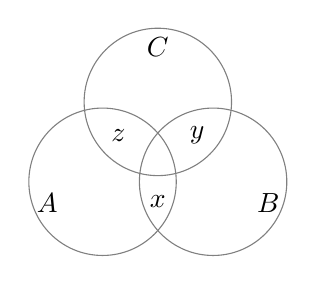
\begin{tikzpicture}[scale=0.78]
\draw[gray] (0,0.75) circle (1.2);
\draw[gray] (-0.9,-0.55) circle (1.2);
\draw[gray] (0.9,-0.55) circle (1.2);
\node at (0,1.65) {$C$};
\node at (-1.8,-0.9) {$A$};
\node at (1.8,-0.9) {$B$};
\node at (-0.64,0.20) {$z$};
\node at (0.64,0.20) {$y$};
\node at (0,-0.88) {$x$};
\end{tikzpicture}
\end{center}
\step{① 集合 $\{1,2,3,4\}$ 中的子集合有 4 个元素，所以从 $1,2,3,4$ 四个元素选 3 个有 $C_4^3=4$ 种方法，将 3 个元素进行全排列有 $P_3^3=3\times2=6$ 种，剩余的一个元素可以分别放入集合 $A$、$B$、$C$，有 3 种，所以此时共有 $3\times4\times6=72$ 种。}
\step{② 集合 $\{1,2,3,4\}$ 中的子集合有 3 个元素，满足集合 $A$、$B$、$C$ 中都只有一个元素。}
\step{所以从 $1,2,3,4$ 四个元素选 3 个有 $C_4^3=4$ 种方法，将 3 个元素进行全排列有 $P_3^3=3\times2=6$ 种，所以此时共有 $4\times6=24$ 种。}
\step{综上，共有 $72+24=96$ 个。}
\solend
\fi

\item 设 $a\in\R$，记 $f(x)=x^2+2x+a$，若关于 $x$ 的不等式 $f(f(x))<0$ 的解集为 $\varnothing$，则 $a$ 的取值范围为 \blankline[4.4em].

\ifanswer
\solbegin
\step{二次函数 $f(x)=x^2+2x+a$ 的开口向上，对称轴为 $x=-1$，所以 $f(x)_{\min}=f(-1)=a-1$，即 $f(x)$ 的值域为 $[a-1,+\infty)$.}
\step{要使不等式 $f(f(x))<0$ 的解集为空集，则 $f(f(x))\geqslant0$ 恒成立，}
\step{所以 $\begin{cases}f(a-1)\geqslant0,\\a-1\geqslant-1,\end{cases}$ 即 $\begin{cases}a^2+a-1\geqslant0,\\a\geqslant0,\end{cases}$}
\step{解得 $a\geqslant\dfrac{\sqrt5-1}{2}$，所以实数 $a$ 的取值范围为 $\left[\dfrac{\sqrt5-1}{2},+\infty\right)$.}
\solend
\fi

\end{enumerate}

\bigsec{二、选择题}

\begin{enumerate}
\setcounter{enumi}{12}

\item 已知关于 $x$ 的不等式 $2x-1>a(x-2)$ 的解集是 $\R$，则数 $a$ 的取值范围是\mbox{（\quad）}

\keepwithprev
A. $a>2$\qquad B. $a=2$

C. $a<2$\qquad D. $a$ 不存在

\ans{$B$}

\item 设 $0<a_1<a_2$，$0<b_1<b_2$，且 $a_1+a_2=b_1+b_2=1$，如果要把 $a_1b_1+a_2b_2$、$a_1b_2+a_2b_1$、$\dfrac12$ 按从小到大的顺序排列，那么排在中间的数是\mbox{（\quad）}

\keepwithprev
A. 一定是 $a_1b_1+a_2b_2$\qquad B. 一定是 $a_1b_2+a_2b_1$

C. 一定是 $\dfrac12$\qquad D. 不能确定，与 $a_1,a_2,b_1,b_2$ 的值有关

\ans{$C$}

\item “$0<a<b$”是“$a-\dfrac1a<b-\dfrac1b$”的\mbox{（\quad）}条件

\keepwithprev
A. 充分不必要\qquad B. 必要不充分

C. 充分必要\qquad D. 既不充分也不必要

\ans{$A$}

\item 在 $n$ 元集合 $S=\{a_1,a_2,\cdots,a_n\}$ 中，设 $x(S)=\dfrac{a_1+a_2+\cdots+a_n}{n}$，若 $S$ 的非空子集 $A$ 满足 $x(A)=x(S)$，则称 $A$ 是集合 $S$ 的一个“平均子集”，并记集合 $S$ 的 $k$ 个“平均子集”的个数为 $f_S(k)$. 已知集合 $S=\{1,2,3,4,5,6,7,8,9\}$，$T=\{-4,-3,-2,-1,0,1,2,3,4\}$，则下列说法错误的是\mbox{（\quad）}

\keepwithprev
A. $f_S(9)=f_T(1)$\qquad B. $f_S(8)=f_T(1)$

C. $f_S(6)=f_T(4)$\qquad D. $f_S(5)=f_T(4)$

\ans{$D$}

\ifanswer
\solbegin
\step{$X(S)=5$，将 $S$ 中的元素分成 5 组 $(1,9)$、$(2,8)$、$(3,7)$、$(4,6)$、$(5)$.}
\step{则 $f_S(1)=C_1^1=1$，$f_S(2)=C_4^1=4$，$f_S(3)=C_1^1C_4^1=4$，$f_S(4)=C_4^2=6$，$f_S(5)=C_1^1C_4^2=6$，同时 $X(T)=0$，将 $T$ 中的元素分成 5 组 $(1,-1)$、$(2,-2)$、$(3,-3)$、$(4,-4)$、$(0)$.}
\step{则 $f_T(1)=C_1^1=1$，$f_T(2)=C_4^1=4$，$f_T(3)=C_1^1C_4^1=4$，$f_T(4)=C_4^2=6$，$f_T(5)=C_1^1C_4^2=6$，$f_T(8)=C_4^4=1$，所以 $f_S(4)=f_S(5)=f_T(4)=6$，故选 D.}
\solend
\fi

\end{enumerate}

\bigsec{三、解答题}

\begin{enumerate}
\setcounter{enumi}{16}

\item 已知集合 $A=\{x\mid x^2-12x+20\leqslant0\}$，$B=\{x\mid2m<x<m+4\}$.

\begin{enumerate}[label=(\arabic*)]
\item 若 $m=3$，求 $A\cup B$；
\item 若 $A\cap B=\varnothing$，求 $m$ 的取值范围.
\end{enumerate}

\ifanswer
\solbegin
\stepm{(1)}{因为 $A=\{x\mid x^2-12x+20\leqslant0\}=\{x\mid2\leqslant x\leqslant10\}$，当 $m=3$ 时，$B=\{x\mid6<x<7\}$，所以 $A\cup B=\{x\mid2\leqslant x\leqslant10\}$.}
\stepm{(2)}{当 $m+4\leqslant2$ 时，$B$ 在 $A$ 的左侧，得 $m\leqslant-2$；当 $2m\geqslant10$ 时，得 $m\geqslant5$；当 $2m\geqslant m+4$ 时，$B=\varnothing$，得 $m\geqslant4$.}
\step{综上，$m\leqslant-2$ 或 $m\geqslant4$.}
\solend
\fi

\item 已知 $a>0$，关于 $x$ 的方程 $\dfrac1{x-2}+\dfrac1{x-1}=\dfrac{\sqrt{ax}}{x^2-3x+2}$ 有且仅有一个实数根，求实数 $a$ 的取值范围.

\ifanswer
\solbegin
\step{由题意得 $x\neq2$，$x\neq1$. 去分母整理得 $2x-3=\sqrt{ax}\geqslant0$，所以 $x\geqslant\dfrac32$，且 $x\neq2$.}
\step{两边平方整理得 $4x^2-(12+a)x+9=0$，判别式 $\Delta=a^2+24a>0$.}
\step{设方程的两个根为 $x_1$、$x_2$，则 $x_1+x_2=\dfrac{12+a}{4}$，$x_1x_2=\dfrac94$.}
\step{当 $0<a<\dfrac12$ 时，方程有一个根在 $\left(\dfrac32,2\right)$ 内，另一个根小于 $\dfrac32$，符合题意；}
\step{当 $a=\dfrac12$ 时，方程的根为 $2$、$\dfrac98$，均不符合题意；}
\step{当 $a>\dfrac12$ 时，方程有一个根大于 $2$，另一个根小于 $\dfrac32$，符合题意。}
\step{综上，实数 $a$ 的取值范围为 $\left(0,\dfrac12\right)\cup\left(\dfrac12,+\infty\right)$.}
\solend
\fi

\item 已知 $a\in\R$，关于 $x$ 的不等式 $ax^2-ax+3>0$ 恒成立.

\begin{enumerate}[label=(\arabic*)]
\item 求实数 $a$ 的取值范围；
\item 在（1）的条件下用反证法证明：三个关于 $x$ 的方程 $x^2+4ax-4a+3=0$，$x^2+(a-1)x+a^2=0$，$x^2+2ax-2a=0$ 中至少有一个方程有实数解.
\end{enumerate}

\ifanswer
\solbegin
\stepm{(1)}{当 $a=0$ 时，$3>0$ 恒成立；当 $a>0$ 时，$\Delta=a^2-12a<0$，解得 $0<a<12$；当 $a<0$ 时，不等式不恒成立。}
\step{综上，$a\in[0,12)$.}
\stepm{(2)}{假设三个方程均无实数解，则}
\step{$\begin{cases}\Delta_1=16a^2+16a-12<0,\\\Delta_2=(a-1)^2-4a^2<0,\\\Delta_3=4a^2+8a<0,\end{cases}$}
\step{解得 $-\dfrac32<a<\dfrac12$，$a<-1$ 或 $a>\dfrac13$，$-2<a<0$.}
\step{由 $a\in[0,12)$，前两个不等式得 $\dfrac13<a<\dfrac12$，第三个不等式得 $-2<a<0$，矛盾。}
\step{所以三个方程中至少有一个方程有实数解。}
\solend
\fi

% 注：原卷条件③按字面未限定 2x∈P_n；若对所有 x∈P_n 都要求 2x∈A，原卷答案 f(4)=4 与之不符。
%     2012 年江苏卷源题将其表述为相对于 P_n 的补集条件；本稿仍照录高一42原文，未替换。
\item 设集合 $P_n=\{1,2,\cdots,n\}$，$n\in\N^*$. 记 $f(n)$ 为同时满足下列条件的集合 $A$ 的个数：

① $A\subseteq P_n$；②若 $x\in A$，则 $2x\notin A$；③若 $x\notin A$，则 $2x\in A$.

\begin{enumerate}[label=(\arabic*)]
\item 求 $f(4)$；
\item 求 $f(n)$ 的解析式（用 $n$ 表示）.
\end{enumerate}

\ifanswer
\solbegin
\stepm{(1)}{当 $n=4$ 时，$P_4=\{1,2,3,4\}$，符合条件的集合 $A$ 为 $\{2\}$、$\{1,4\}$、$\{2,3\}$、$\{1,3,4\}$，故 $f(4)=4$.}
\stepm{(2)}{任取偶数 $x\in P_n$，将 $x$ 除以 2，若商仍为偶数，再除以 2，经过 $k$ 次后商必为奇数，此时商记为 $m$.}
\step{于是 $x=m\cdot2^k$，其中 $m$ 为奇数，$k\in\N^*$.}
\step{由条件得，若 $m\in A$，则 $x\in A\Longleftrightarrow k$ 为偶数；若 $m\notin A$，则 $x\in A\Longleftrightarrow k$ 为奇数。}
\step{因此每个奇数 $m\in P_n$ 是否属于 $A$ 可任意选择，且确定后其所有倍数的归属也唯一确定。}
\step{当 $n$ 为偶数时，$P_n$ 中奇数有 $\dfrac n2$ 个；当 $n$ 为奇数时，$P_n$ 中奇数有 $\dfrac{n+1}{2}$ 个。}
\step{所以 $f(n)=\begin{cases}2^{\frac n2},&n\text{ 为偶数},\\2^{\frac{n+1}{2}},&n\text{ 为奇数} .\end{cases}$}
\solend
\fi

\item 设 $S_n=\{(x_1,x_2,\cdots,x_n)\mid x_i\in\{0,1\},\ i=1,2,\cdots,n\}$（$n$ 为正整数），对任意的 $\alpha=(x_1,x_2,\cdots,x_n)$，$\beta=(y_1,y_2,\cdots,y_n)$，定义 $\alpha\cdot\beta=x_1y_1+x_2y_2+\cdots+x_ny_n$.

\begin{enumerate}[label=(\arabic*)]
\item 当 $n=3$ 时，$\alpha=(1,1,0)$，$\beta=(1,0,1)$，求 $\alpha\cdot\beta$；
\item 当 $n=3$ 时，集合 $A\subseteq S_n$，对任意 $\alpha,\beta\in A$，$\alpha\cdot\beta$ 均为偶数，求 $A$ 中元素个数的最大值；
\item 集合 $A\subseteq S_n$，对任意 $\alpha,\beta\in A$，$\alpha\neq\beta$，均有 $\alpha\cdot\beta\neq0$，求 $A$ 中元素个数的最大值.
\end{enumerate}

\ifanswer
\solbegin
\stepm{(1)}{当 $n=3$ 时，$\alpha\cdot\beta=x_1y_1+x_2y_2+x_3y_3=1\times1+1\times0+0\times1=1$.}
\stepm{(2)}{因为 $\alpha\cdot\beta=x_1y_1+x_2y_2+x_3y_3$ 均为偶数，所以结果为 $0$ 或 $2$.}
\step{当 $\alpha\cdot\beta=0$，则 $A$ 中元素个数最多有 $4$ 个；当 $\alpha\cdot\beta=2$，则 $A$ 中元素个数最多有 $1$ 个。}
\step{综上，$A$ 中元素个数的最大值为 $4$.}
\stepm{(3)}{若 $\alpha=(x_1,x_2,\cdots,x_n)\in A$，令 $\gamma=(1-x_1,1-x_2,\cdots,1-x_n)$，则 $\alpha\cdot\gamma=0$.}
\step{因为 $\alpha\cdot\beta\neq0$，$\alpha\in A$，所以 $\gamma\notin A$.}
\step{因为 $S_n$ 中有 $2^n$ 个元素，所以 $A$ 中元素个数最多有 $\dfrac{2^n}{2}=2^{n-1}$ 个。}
\step{综上，$A$ 中元素个数的最大值为 $2^{n-1}$.}
\solend
\fi

\end{enumerate}

\end{document}
"
% 紧凑版：xelatex "\def\iscompact{1}% 高一42_复旦附中_周末作业4.tex
%   —— 高一上数学“2026-2027 年复旦附中高一上周末作业 4”（试卷版/答案版）
% 试卷版：xelatex 高一42_复旦附中_周末作业4.tex
% 答案版：xelatex "\def\isanswer{1}\input{高一42_复旦附中_周末作业4.tex}"
% 紧凑版：xelatex "\def\iscompact{1}\input{高一42_复旦附中_周末作业4.tex}"
%
% 原始材料：微信公众号“魔都数学加油站”文章，作者破晓，2026-10-01 21:37 发布；
% 文章标题“27学年高一42——2026-2027年上海市复旦附中高一上周末作业4”；
% URL：https://mp.weixin.qq.com/s/nZ8aTd6K9OLS9S4-J-O7lA。
% 正文为 8 张 PNG 页（第 02、08 页 2560×3620，其余六页 4762×6735）。题目、答案及解析均据原图转录。
%
% 卷面标题行印作“2026-2027 年复旦附中高一上周末作业 4”，未印“上海市”；本稿标题照卷面，
% 年份区间按全稿惯例排 en dash。卷面未印副标题，本稿按“知识模块”口径标为“集合与常用逻辑用语、不等式”。
%
% 与原卷的排版差异：
%   ① 原文题号从第 3 题开始，本稿保留原题号；
%   ② 原卷的“一、填空题”“二、选择题”“三、解答题”改排为全稿统一的大节标题；
%   ③ 原卷填空横线统一排为 \blankline[4.4em]；选择题答案统一用 \ans{} 排在选项之后，
%      答案版与试卷版分离；原卷题目下方印出的【答案】、【解析】在答案版中排出；
%   ④ 原卷的粉色斜水印“魔都数学加油站”未录入；第 11 题解析中的三集合示意图以 TikZ 重绘。
%
% 原卷存疑处（照录原文）：
%   ① 第 5 题印出的答案为 $P>Q$，但取 $a=8,b=1$ 即得 $P=1<Q=\sqrt[3]{7}$；本稿照录；
%   ② 第 16 题解析按对称数对计数，印出 f_T(4)=C_4^2=6 并据此“故选 D”；但 T 中还可见
%      {0,1,2,-3} 这类和为 0 的四元子集，原卷的计数及选项结论疑有遗漏，本稿保留原解析和答案；
%   ③ 第 20 题的条件③印作“若 x∉A，则 2x∈A”，未明确限定 2x∈P_n；按此字面读法，f(4)
%      与【解析】列出的四个集合不符，而原题源 2012 年江苏卷明确写补集相对 P_n。
%      本稿照录原卷，不改条件，也不以源题替换；
%   ④ 第 21(2) 题题干未写 α≠β，解析结论为 4；此处照卷面题干与结论录入。
\documentclass[a4paper,11pt]{article}
\usepackage{common}

\begin{document}

\examtitlest[4]{2026--2027 年复旦附中高一上周末作业 4}{集合与常用逻辑用语、不等式}

\bigsec{一、填空题}

\begin{enumerate}
\setcounter{enumi}{2}

\item 若 $-1<x<y<2$，则 $x-y$ 的取值范围为 \blankline[4.4em].

\ifanswer
\solbegin
\step{$(-3,0)$.}
\solend
\fi

\item 已知 $c>d$，若 $ac+bd>bc+ad$，则 $a-b$ 与 $0$ 的大小关系是 \blankline[4.4em].

\ifanswer
\solbegin
\step{$a-b>0$.}
\solend
\fi

\item 已知 $a>b>0$，$P=\sqrt[3]{a}-\sqrt[3]{b}$，$Q=\sqrt[3]{a-b}$，则 $P$、$Q$ 的大小关系是 \blankline[4.4em].

\ifanswer
\solbegin
\step{$P>Q$.}
\solend
\fi

\item 对任意的实数 $x$，不等式 $x+|x-1|\geqslant m$ 恒成立，则实数 $m$ 的取值范围是 \blankline[4.4em].

\ifanswer
\solbegin
\step{令 $f(x)=x+|x-1|=\begin{cases}2x-1,&x\geqslant1,\\1,&x<1.\end{cases}$}
\step{当 $x\geqslant1$ 时，不等式变为 $2x-1\geqslant m$，显然满足题意；}
\step{当 $x<1$ 时，不等式变为 $1\geqslant m$，解得 $m\leqslant1$.}
\step{综上，$m\leqslant1$.}
\solend
\fi

\item 若“存在 $x\in\{x\mid1\leqslant x\leqslant2\}$，使得 $3x+a+1\geqslant0$”是命题，则实数 $a$ 的取值范围是 \blankline[4.4em].

\ifanswer
\solbegin
\step{由题意得 $6+a+1\geqslant0$，所以 $a\geqslant-7$.}
\solend
\fi

\item 已知关于 $x$ 的不等式 $ax-b\leqslant0$ 的解集是 $[2,+\infty)$，则关于 $x$ 的不等式
$ax^2+(3a-b)x-3b<0$ 的解集是 \blankline[4.4em].

\ifanswer
\solbegin
\step{由题意得 $a<0$，且 $\dfrac ba=2$，所以 $b=2a$.}
\step{当 $a<0$ 时，$ax^2+(3a-b)x-3b<0$ 等价于 $x^2+x-6>0$，}
\step{解得 $x\in(-\infty,-3)\cup(2,+\infty)$.}
\solend
\fi

\item 若关于 $x$ 的不等式 $(k^2+4k-5)x^2+4(1-k)x+3>0$ 恒成立，则实数 $k$ 的取值范围是 \blankline[4.4em].

\ifanswer
\solbegin
\step{当 $k=-5$ 时，不等式变为 $24x+3>0$，显然不满足题意，所以 $k\neq-5$.}
\step{当 $k=1$ 时，不等式变为 $3>0$，显然满足题意，所以 $k=1$.}
\step{当 $k^2+4k-5\neq0$ 时，有 $\begin{cases}k^2+4k-5>0,\\\Delta<0,\end{cases}$}
\step{即 $\begin{cases}k^2+4k-5>0,\\4(k-1)(k-19)<0,\end{cases}$，解得 $1<k<19$.}
\step{综上，实数 $k$ 的取值范围是 $[1,19)$.}
\solend
\fi

\item 设 $a\in\R$，集合 $A=\{x\mid x^2-ax+a\leqslant0\}$，若 $A\cap\N\neq\varnothing$，则 $a$ 的取值范围是 \blankline[4.4em].

\ifanswer
\solbegin
\step{$(-\infty,0]\cup[4,+\infty)$.}
\solend
\fi

\item 用 $|S|$ 表示集合 $S$ 中的元素的个数，设 $A$、$B$、$C$ 为集合，称 $(A,B,C)$ 为有序三元组。如果集合 $A$、$B$、$C$ 满足 $|A\cap B|=|B\cap C|=|C\cap A|=1$，且 $|A\cap B\cap C|=0$，则称有序三元组 $(A,B,C)$ 为最小交。由集合 $\{1,2,3,4\}$ 的子集构成的所有有序三元组中，最小交的有序三元组的个数为 \blankline[4.4em].

\ifanswer
\solbegin
\step{设 $A\cap B=\{x\}$，$B\cap C=\{y\}$，$C\cap A=\{z\}$，则 $x,y,z\in\{1,2,3,4\}$，且 $x,y,z$ 互不相同。}
\begin{center}
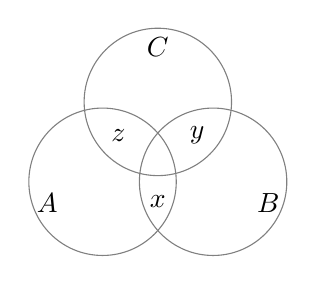
\begin{tikzpicture}[scale=0.78]
\draw[gray] (0,0.75) circle (1.2);
\draw[gray] (-0.9,-0.55) circle (1.2);
\draw[gray] (0.9,-0.55) circle (1.2);
\node at (0,1.65) {$C$};
\node at (-1.8,-0.9) {$A$};
\node at (1.8,-0.9) {$B$};
\node at (-0.64,0.20) {$z$};
\node at (0.64,0.20) {$y$};
\node at (0,-0.88) {$x$};
\end{tikzpicture}
\end{center}
\step{① 集合 $\{1,2,3,4\}$ 中的子集合有 4 个元素，所以从 $1,2,3,4$ 四个元素选 3 个有 $C_4^3=4$ 种方法，将 3 个元素进行全排列有 $P_3^3=3\times2=6$ 种，剩余的一个元素可以分别放入集合 $A$、$B$、$C$，有 3 种，所以此时共有 $3\times4\times6=72$ 种。}
\step{② 集合 $\{1,2,3,4\}$ 中的子集合有 3 个元素，满足集合 $A$、$B$、$C$ 中都只有一个元素。}
\step{所以从 $1,2,3,4$ 四个元素选 3 个有 $C_4^3=4$ 种方法，将 3 个元素进行全排列有 $P_3^3=3\times2=6$ 种，所以此时共有 $4\times6=24$ 种。}
\step{综上，共有 $72+24=96$ 个。}
\solend
\fi

\item 设 $a\in\R$，记 $f(x)=x^2+2x+a$，若关于 $x$ 的不等式 $f(f(x))<0$ 的解集为 $\varnothing$，则 $a$ 的取值范围为 \blankline[4.4em].

\ifanswer
\solbegin
\step{二次函数 $f(x)=x^2+2x+a$ 的开口向上，对称轴为 $x=-1$，所以 $f(x)_{\min}=f(-1)=a-1$，即 $f(x)$ 的值域为 $[a-1,+\infty)$.}
\step{要使不等式 $f(f(x))<0$ 的解集为空集，则 $f(f(x))\geqslant0$ 恒成立，}
\step{所以 $\begin{cases}f(a-1)\geqslant0,\\a-1\geqslant-1,\end{cases}$ 即 $\begin{cases}a^2+a-1\geqslant0,\\a\geqslant0,\end{cases}$}
\step{解得 $a\geqslant\dfrac{\sqrt5-1}{2}$，所以实数 $a$ 的取值范围为 $\left[\dfrac{\sqrt5-1}{2},+\infty\right)$.}
\solend
\fi

\end{enumerate}

\bigsec{二、选择题}

\begin{enumerate}
\setcounter{enumi}{12}

\item 已知关于 $x$ 的不等式 $2x-1>a(x-2)$ 的解集是 $\R$，则数 $a$ 的取值范围是\mbox{（\quad）}

\keepwithprev
A. $a>2$\qquad B. $a=2$

C. $a<2$\qquad D. $a$ 不存在

\ans{$B$}

\item 设 $0<a_1<a_2$，$0<b_1<b_2$，且 $a_1+a_2=b_1+b_2=1$，如果要把 $a_1b_1+a_2b_2$、$a_1b_2+a_2b_1$、$\dfrac12$ 按从小到大的顺序排列，那么排在中间的数是\mbox{（\quad）}

\keepwithprev
A. 一定是 $a_1b_1+a_2b_2$\qquad B. 一定是 $a_1b_2+a_2b_1$

C. 一定是 $\dfrac12$\qquad D. 不能确定，与 $a_1,a_2,b_1,b_2$ 的值有关

\ans{$C$}

\item “$0<a<b$”是“$a-\dfrac1a<b-\dfrac1b$”的\mbox{（\quad）}条件

\keepwithprev
A. 充分不必要\qquad B. 必要不充分

C. 充分必要\qquad D. 既不充分也不必要

\ans{$A$}

\item 在 $n$ 元集合 $S=\{a_1,a_2,\cdots,a_n\}$ 中，设 $x(S)=\dfrac{a_1+a_2+\cdots+a_n}{n}$，若 $S$ 的非空子集 $A$ 满足 $x(A)=x(S)$，则称 $A$ 是集合 $S$ 的一个“平均子集”，并记集合 $S$ 的 $k$ 个“平均子集”的个数为 $f_S(k)$. 已知集合 $S=\{1,2,3,4,5,6,7,8,9\}$，$T=\{-4,-3,-2,-1,0,1,2,3,4\}$，则下列说法错误的是\mbox{（\quad）}

\keepwithprev
A. $f_S(9)=f_T(1)$\qquad B. $f_S(8)=f_T(1)$

C. $f_S(6)=f_T(4)$\qquad D. $f_S(5)=f_T(4)$

\ans{$D$}

\ifanswer
\solbegin
\step{$X(S)=5$，将 $S$ 中的元素分成 5 组 $(1,9)$、$(2,8)$、$(3,7)$、$(4,6)$、$(5)$.}
\step{则 $f_S(1)=C_1^1=1$，$f_S(2)=C_4^1=4$，$f_S(3)=C_1^1C_4^1=4$，$f_S(4)=C_4^2=6$，$f_S(5)=C_1^1C_4^2=6$，同时 $X(T)=0$，将 $T$ 中的元素分成 5 组 $(1,-1)$、$(2,-2)$、$(3,-3)$、$(4,-4)$、$(0)$.}
\step{则 $f_T(1)=C_1^1=1$，$f_T(2)=C_4^1=4$，$f_T(3)=C_1^1C_4^1=4$，$f_T(4)=C_4^2=6$，$f_T(5)=C_1^1C_4^2=6$，$f_T(8)=C_4^4=1$，所以 $f_S(4)=f_S(5)=f_T(4)=6$，故选 D.}
\solend
\fi

\end{enumerate}

\bigsec{三、解答题}

\begin{enumerate}
\setcounter{enumi}{16}

\item 已知集合 $A=\{x\mid x^2-12x+20\leqslant0\}$，$B=\{x\mid2m<x<m+4\}$.

\begin{enumerate}[label=(\arabic*)]
\item 若 $m=3$，求 $A\cup B$；
\item 若 $A\cap B=\varnothing$，求 $m$ 的取值范围.
\end{enumerate}

\ifanswer
\solbegin
\stepm{(1)}{因为 $A=\{x\mid x^2-12x+20\leqslant0\}=\{x\mid2\leqslant x\leqslant10\}$，当 $m=3$ 时，$B=\{x\mid6<x<7\}$，所以 $A\cup B=\{x\mid2\leqslant x\leqslant10\}$.}
\stepm{(2)}{当 $m+4\leqslant2$ 时，$B$ 在 $A$ 的左侧，得 $m\leqslant-2$；当 $2m\geqslant10$ 时，得 $m\geqslant5$；当 $2m\geqslant m+4$ 时，$B=\varnothing$，得 $m\geqslant4$.}
\step{综上，$m\leqslant-2$ 或 $m\geqslant4$.}
\solend
\fi

\item 已知 $a>0$，关于 $x$ 的方程 $\dfrac1{x-2}+\dfrac1{x-1}=\dfrac{\sqrt{ax}}{x^2-3x+2}$ 有且仅有一个实数根，求实数 $a$ 的取值范围.

\ifanswer
\solbegin
\step{由题意得 $x\neq2$，$x\neq1$. 去分母整理得 $2x-3=\sqrt{ax}\geqslant0$，所以 $x\geqslant\dfrac32$，且 $x\neq2$.}
\step{两边平方整理得 $4x^2-(12+a)x+9=0$，判别式 $\Delta=a^2+24a>0$.}
\step{设方程的两个根为 $x_1$、$x_2$，则 $x_1+x_2=\dfrac{12+a}{4}$，$x_1x_2=\dfrac94$.}
\step{当 $0<a<\dfrac12$ 时，方程有一个根在 $\left(\dfrac32,2\right)$ 内，另一个根小于 $\dfrac32$，符合题意；}
\step{当 $a=\dfrac12$ 时，方程的根为 $2$、$\dfrac98$，均不符合题意；}
\step{当 $a>\dfrac12$ 时，方程有一个根大于 $2$，另一个根小于 $\dfrac32$，符合题意。}
\step{综上，实数 $a$ 的取值范围为 $\left(0,\dfrac12\right)\cup\left(\dfrac12,+\infty\right)$.}
\solend
\fi

\item 已知 $a\in\R$，关于 $x$ 的不等式 $ax^2-ax+3>0$ 恒成立.

\begin{enumerate}[label=(\arabic*)]
\item 求实数 $a$ 的取值范围；
\item 在（1）的条件下用反证法证明：三个关于 $x$ 的方程 $x^2+4ax-4a+3=0$，$x^2+(a-1)x+a^2=0$，$x^2+2ax-2a=0$ 中至少有一个方程有实数解.
\end{enumerate}

\ifanswer
\solbegin
\stepm{(1)}{当 $a=0$ 时，$3>0$ 恒成立；当 $a>0$ 时，$\Delta=a^2-12a<0$，解得 $0<a<12$；当 $a<0$ 时，不等式不恒成立。}
\step{综上，$a\in[0,12)$.}
\stepm{(2)}{假设三个方程均无实数解，则}
\step{$\begin{cases}\Delta_1=16a^2+16a-12<0,\\\Delta_2=(a-1)^2-4a^2<0,\\\Delta_3=4a^2+8a<0,\end{cases}$}
\step{解得 $-\dfrac32<a<\dfrac12$，$a<-1$ 或 $a>\dfrac13$，$-2<a<0$.}
\step{由 $a\in[0,12)$，前两个不等式得 $\dfrac13<a<\dfrac12$，第三个不等式得 $-2<a<0$，矛盾。}
\step{所以三个方程中至少有一个方程有实数解。}
\solend
\fi

% 注：原卷条件③按字面未限定 2x∈P_n；若对所有 x∈P_n 都要求 2x∈A，原卷答案 f(4)=4 与之不符。
%     2012 年江苏卷源题将其表述为相对于 P_n 的补集条件；本稿仍照录高一42原文，未替换。
\item 设集合 $P_n=\{1,2,\cdots,n\}$，$n\in\N^*$. 记 $f(n)$ 为同时满足下列条件的集合 $A$ 的个数：

① $A\subseteq P_n$；②若 $x\in A$，则 $2x\notin A$；③若 $x\notin A$，则 $2x\in A$.

\begin{enumerate}[label=(\arabic*)]
\item 求 $f(4)$；
\item 求 $f(n)$ 的解析式（用 $n$ 表示）.
\end{enumerate}

\ifanswer
\solbegin
\stepm{(1)}{当 $n=4$ 时，$P_4=\{1,2,3,4\}$，符合条件的集合 $A$ 为 $\{2\}$、$\{1,4\}$、$\{2,3\}$、$\{1,3,4\}$，故 $f(4)=4$.}
\stepm{(2)}{任取偶数 $x\in P_n$，将 $x$ 除以 2，若商仍为偶数，再除以 2，经过 $k$ 次后商必为奇数，此时商记为 $m$.}
\step{于是 $x=m\cdot2^k$，其中 $m$ 为奇数，$k\in\N^*$.}
\step{由条件得，若 $m\in A$，则 $x\in A\Longleftrightarrow k$ 为偶数；若 $m\notin A$，则 $x\in A\Longleftrightarrow k$ 为奇数。}
\step{因此每个奇数 $m\in P_n$ 是否属于 $A$ 可任意选择，且确定后其所有倍数的归属也唯一确定。}
\step{当 $n$ 为偶数时，$P_n$ 中奇数有 $\dfrac n2$ 个；当 $n$ 为奇数时，$P_n$ 中奇数有 $\dfrac{n+1}{2}$ 个。}
\step{所以 $f(n)=\begin{cases}2^{\frac n2},&n\text{ 为偶数},\\2^{\frac{n+1}{2}},&n\text{ 为奇数} .\end{cases}$}
\solend
\fi

\item 设 $S_n=\{(x_1,x_2,\cdots,x_n)\mid x_i\in\{0,1\},\ i=1,2,\cdots,n\}$（$n$ 为正整数），对任意的 $\alpha=(x_1,x_2,\cdots,x_n)$，$\beta=(y_1,y_2,\cdots,y_n)$，定义 $\alpha\cdot\beta=x_1y_1+x_2y_2+\cdots+x_ny_n$.

\begin{enumerate}[label=(\arabic*)]
\item 当 $n=3$ 时，$\alpha=(1,1,0)$，$\beta=(1,0,1)$，求 $\alpha\cdot\beta$；
\item 当 $n=3$ 时，集合 $A\subseteq S_n$，对任意 $\alpha,\beta\in A$，$\alpha\cdot\beta$ 均为偶数，求 $A$ 中元素个数的最大值；
\item 集合 $A\subseteq S_n$，对任意 $\alpha,\beta\in A$，$\alpha\neq\beta$，均有 $\alpha\cdot\beta\neq0$，求 $A$ 中元素个数的最大值.
\end{enumerate}

\ifanswer
\solbegin
\stepm{(1)}{当 $n=3$ 时，$\alpha\cdot\beta=x_1y_1+x_2y_2+x_3y_3=1\times1+1\times0+0\times1=1$.}
\stepm{(2)}{因为 $\alpha\cdot\beta=x_1y_1+x_2y_2+x_3y_3$ 均为偶数，所以结果为 $0$ 或 $2$.}
\step{当 $\alpha\cdot\beta=0$，则 $A$ 中元素个数最多有 $4$ 个；当 $\alpha\cdot\beta=2$，则 $A$ 中元素个数最多有 $1$ 个。}
\step{综上，$A$ 中元素个数的最大值为 $4$.}
\stepm{(3)}{若 $\alpha=(x_1,x_2,\cdots,x_n)\in A$，令 $\gamma=(1-x_1,1-x_2,\cdots,1-x_n)$，则 $\alpha\cdot\gamma=0$.}
\step{因为 $\alpha\cdot\beta\neq0$，$\alpha\in A$，所以 $\gamma\notin A$.}
\step{因为 $S_n$ 中有 $2^n$ 个元素，所以 $A$ 中元素个数最多有 $\dfrac{2^n}{2}=2^{n-1}$ 个。}
\step{综上，$A$ 中元素个数的最大值为 $2^{n-1}$.}
\solend
\fi

\end{enumerate}

\end{document}
"
%
% 原始材料：微信公众号“魔都数学加油站”文章，作者破晓，2026-10-01 21:37 发布；
% 文章标题“27学年高一42——2026-2027年上海市复旦附中高一上周末作业4”；
% URL：https://mp.weixin.qq.com/s/nZ8aTd6K9OLS9S4-J-O7lA。
% 正文为 8 张 PNG 页（第 02、08 页 2560×3620，其余六页 4762×6735）。题目、答案及解析均据原图转录。
%
% 卷面标题行印作“2026-2027 年复旦附中高一上周末作业 4”，未印“上海市”；本稿标题照卷面，
% 年份区间按全稿惯例排 en dash。卷面未印副标题，本稿按“知识模块”口径标为“集合与常用逻辑用语、不等式”。
%
% 与原卷的排版差异：
%   ① 原文题号从第 3 题开始，本稿保留原题号；
%   ② 原卷的“一、填空题”“二、选择题”“三、解答题”改排为全稿统一的大节标题；
%   ③ 原卷填空横线统一排为 \blankline[4.4em]；选择题答案统一用 \ans{} 排在选项之后，
%      答案版与试卷版分离；原卷题目下方印出的【答案】、【解析】在答案版中排出；
%   ④ 原卷的粉色斜水印“魔都数学加油站”未录入；第 11 题解析中的三集合示意图以 TikZ 重绘。
%
% 原卷存疑处（照录原文）：
%   ① 第 5 题印出的答案为 $P>Q$，但取 $a=8,b=1$ 即得 $P=1<Q=\sqrt[3]{7}$；本稿照录；
%   ② 第 16 题解析按对称数对计数，印出 f_T(4)=C_4^2=6 并据此“故选 D”；但 T 中还可见
%      {0,1,2,-3} 这类和为 0 的四元子集，原卷的计数及选项结论疑有遗漏，本稿保留原解析和答案；
%   ③ 第 20 题的条件③印作“若 x∉A，则 2x∈A”，未明确限定 2x∈P_n；按此字面读法，f(4)
%      与【解析】列出的四个集合不符，而原题源 2012 年江苏卷明确写补集相对 P_n。
%      本稿照录原卷，不改条件，也不以源题替换；
%   ④ 第 21(2) 题题干未写 α≠β，解析结论为 4；此处照卷面题干与结论录入。
\documentclass[a4paper,11pt]{article}
\usepackage{common}

\begin{document}

\examtitlest[4]{2026--2027 年复旦附中高一上周末作业 4}{集合与常用逻辑用语、不等式}

\bigsec{一、填空题}

\begin{enumerate}
\setcounter{enumi}{2}

\item 若 $-1<x<y<2$，则 $x-y$ 的取值范围为 \blankline[4.4em].

\ifanswer
\solbegin
\step{$(-3,0)$.}
\solend
\fi

\item 已知 $c>d$，若 $ac+bd>bc+ad$，则 $a-b$ 与 $0$ 的大小关系是 \blankline[4.4em].

\ifanswer
\solbegin
\step{$a-b>0$.}
\solend
\fi

\item 已知 $a>b>0$，$P=\sqrt[3]{a}-\sqrt[3]{b}$，$Q=\sqrt[3]{a-b}$，则 $P$、$Q$ 的大小关系是 \blankline[4.4em].

\ifanswer
\solbegin
\step{$P>Q$.}
\solend
\fi

\item 对任意的实数 $x$，不等式 $x+|x-1|\geqslant m$ 恒成立，则实数 $m$ 的取值范围是 \blankline[4.4em].

\ifanswer
\solbegin
\step{令 $f(x)=x+|x-1|=\begin{cases}2x-1,&x\geqslant1,\\1,&x<1.\end{cases}$}
\step{当 $x\geqslant1$ 时，不等式变为 $2x-1\geqslant m$，显然满足题意；}
\step{当 $x<1$ 时，不等式变为 $1\geqslant m$，解得 $m\leqslant1$.}
\step{综上，$m\leqslant1$.}
\solend
\fi

\item 若“存在 $x\in\{x\mid1\leqslant x\leqslant2\}$，使得 $3x+a+1\geqslant0$”是命题，则实数 $a$ 的取值范围是 \blankline[4.4em].

\ifanswer
\solbegin
\step{由题意得 $6+a+1\geqslant0$，所以 $a\geqslant-7$.}
\solend
\fi

\item 已知关于 $x$ 的不等式 $ax-b\leqslant0$ 的解集是 $[2,+\infty)$，则关于 $x$ 的不等式
$ax^2+(3a-b)x-3b<0$ 的解集是 \blankline[4.4em].

\ifanswer
\solbegin
\step{由题意得 $a<0$，且 $\dfrac ba=2$，所以 $b=2a$.}
\step{当 $a<0$ 时，$ax^2+(3a-b)x-3b<0$ 等价于 $x^2+x-6>0$，}
\step{解得 $x\in(-\infty,-3)\cup(2,+\infty)$.}
\solend
\fi

\item 若关于 $x$ 的不等式 $(k^2+4k-5)x^2+4(1-k)x+3>0$ 恒成立，则实数 $k$ 的取值范围是 \blankline[4.4em].

\ifanswer
\solbegin
\step{当 $k=-5$ 时，不等式变为 $24x+3>0$，显然不满足题意，所以 $k\neq-5$.}
\step{当 $k=1$ 时，不等式变为 $3>0$，显然满足题意，所以 $k=1$.}
\step{当 $k^2+4k-5\neq0$ 时，有 $\begin{cases}k^2+4k-5>0,\\\Delta<0,\end{cases}$}
\step{即 $\begin{cases}k^2+4k-5>0,\\4(k-1)(k-19)<0,\end{cases}$，解得 $1<k<19$.}
\step{综上，实数 $k$ 的取值范围是 $[1,19)$.}
\solend
\fi

\item 设 $a\in\R$，集合 $A=\{x\mid x^2-ax+a\leqslant0\}$，若 $A\cap\N\neq\varnothing$，则 $a$ 的取值范围是 \blankline[4.4em].

\ifanswer
\solbegin
\step{$(-\infty,0]\cup[4,+\infty)$.}
\solend
\fi

\item 用 $|S|$ 表示集合 $S$ 中的元素的个数，设 $A$、$B$、$C$ 为集合，称 $(A,B,C)$ 为有序三元组。如果集合 $A$、$B$、$C$ 满足 $|A\cap B|=|B\cap C|=|C\cap A|=1$，且 $|A\cap B\cap C|=0$，则称有序三元组 $(A,B,C)$ 为最小交。由集合 $\{1,2,3,4\}$ 的子集构成的所有有序三元组中，最小交的有序三元组的个数为 \blankline[4.4em].

\ifanswer
\solbegin
\step{设 $A\cap B=\{x\}$，$B\cap C=\{y\}$，$C\cap A=\{z\}$，则 $x,y,z\in\{1,2,3,4\}$，且 $x,y,z$ 互不相同。}
\begin{center}
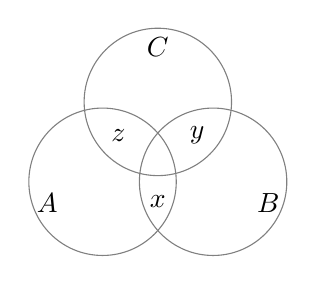
\begin{tikzpicture}[scale=0.78]
\draw[gray] (0,0.75) circle (1.2);
\draw[gray] (-0.9,-0.55) circle (1.2);
\draw[gray] (0.9,-0.55) circle (1.2);
\node at (0,1.65) {$C$};
\node at (-1.8,-0.9) {$A$};
\node at (1.8,-0.9) {$B$};
\node at (-0.64,0.20) {$z$};
\node at (0.64,0.20) {$y$};
\node at (0,-0.88) {$x$};
\end{tikzpicture}
\end{center}
\step{① 集合 $\{1,2,3,4\}$ 中的子集合有 4 个元素，所以从 $1,2,3,4$ 四个元素选 3 个有 $C_4^3=4$ 种方法，将 3 个元素进行全排列有 $P_3^3=3\times2=6$ 种，剩余的一个元素可以分别放入集合 $A$、$B$、$C$，有 3 种，所以此时共有 $3\times4\times6=72$ 种。}
\step{② 集合 $\{1,2,3,4\}$ 中的子集合有 3 个元素，满足集合 $A$、$B$、$C$ 中都只有一个元素。}
\step{所以从 $1,2,3,4$ 四个元素选 3 个有 $C_4^3=4$ 种方法，将 3 个元素进行全排列有 $P_3^3=3\times2=6$ 种，所以此时共有 $4\times6=24$ 种。}
\step{综上，共有 $72+24=96$ 个。}
\solend
\fi

\item 设 $a\in\R$，记 $f(x)=x^2+2x+a$，若关于 $x$ 的不等式 $f(f(x))<0$ 的解集为 $\varnothing$，则 $a$ 的取值范围为 \blankline[4.4em].

\ifanswer
\solbegin
\step{二次函数 $f(x)=x^2+2x+a$ 的开口向上，对称轴为 $x=-1$，所以 $f(x)_{\min}=f(-1)=a-1$，即 $f(x)$ 的值域为 $[a-1,+\infty)$.}
\step{要使不等式 $f(f(x))<0$ 的解集为空集，则 $f(f(x))\geqslant0$ 恒成立，}
\step{所以 $\begin{cases}f(a-1)\geqslant0,\\a-1\geqslant-1,\end{cases}$ 即 $\begin{cases}a^2+a-1\geqslant0,\\a\geqslant0,\end{cases}$}
\step{解得 $a\geqslant\dfrac{\sqrt5-1}{2}$，所以实数 $a$ 的取值范围为 $\left[\dfrac{\sqrt5-1}{2},+\infty\right)$.}
\solend
\fi

\end{enumerate}

\bigsec{二、选择题}

\begin{enumerate}
\setcounter{enumi}{12}

\item 已知关于 $x$ 的不等式 $2x-1>a(x-2)$ 的解集是 $\R$，则数 $a$ 的取值范围是\mbox{（\quad）}

\keepwithprev
A. $a>2$\qquad B. $a=2$

C. $a<2$\qquad D. $a$ 不存在

\ans{$B$}

\item 设 $0<a_1<a_2$，$0<b_1<b_2$，且 $a_1+a_2=b_1+b_2=1$，如果要把 $a_1b_1+a_2b_2$、$a_1b_2+a_2b_1$、$\dfrac12$ 按从小到大的顺序排列，那么排在中间的数是\mbox{（\quad）}

\keepwithprev
A. 一定是 $a_1b_1+a_2b_2$\qquad B. 一定是 $a_1b_2+a_2b_1$

C. 一定是 $\dfrac12$\qquad D. 不能确定，与 $a_1,a_2,b_1,b_2$ 的值有关

\ans{$C$}

\item “$0<a<b$”是“$a-\dfrac1a<b-\dfrac1b$”的\mbox{（\quad）}条件

\keepwithprev
A. 充分不必要\qquad B. 必要不充分

C. 充分必要\qquad D. 既不充分也不必要

\ans{$A$}

\item 在 $n$ 元集合 $S=\{a_1,a_2,\cdots,a_n\}$ 中，设 $x(S)=\dfrac{a_1+a_2+\cdots+a_n}{n}$，若 $S$ 的非空子集 $A$ 满足 $x(A)=x(S)$，则称 $A$ 是集合 $S$ 的一个“平均子集”，并记集合 $S$ 的 $k$ 个“平均子集”的个数为 $f_S(k)$. 已知集合 $S=\{1,2,3,4,5,6,7,8,9\}$，$T=\{-4,-3,-2,-1,0,1,2,3,4\}$，则下列说法错误的是\mbox{（\quad）}

\keepwithprev
A. $f_S(9)=f_T(1)$\qquad B. $f_S(8)=f_T(1)$

C. $f_S(6)=f_T(4)$\qquad D. $f_S(5)=f_T(4)$

\ans{$D$}

\ifanswer
\solbegin
\step{$X(S)=5$，将 $S$ 中的元素分成 5 组 $(1,9)$、$(2,8)$、$(3,7)$、$(4,6)$、$(5)$.}
\step{则 $f_S(1)=C_1^1=1$，$f_S(2)=C_4^1=4$，$f_S(3)=C_1^1C_4^1=4$，$f_S(4)=C_4^2=6$，$f_S(5)=C_1^1C_4^2=6$，同时 $X(T)=0$，将 $T$ 中的元素分成 5 组 $(1,-1)$、$(2,-2)$、$(3,-3)$、$(4,-4)$、$(0)$.}
\step{则 $f_T(1)=C_1^1=1$，$f_T(2)=C_4^1=4$，$f_T(3)=C_1^1C_4^1=4$，$f_T(4)=C_4^2=6$，$f_T(5)=C_1^1C_4^2=6$，$f_T(8)=C_4^4=1$，所以 $f_S(4)=f_S(5)=f_T(4)=6$，故选 D.}
\solend
\fi

\end{enumerate}

\bigsec{三、解答题}

\begin{enumerate}
\setcounter{enumi}{16}

\item 已知集合 $A=\{x\mid x^2-12x+20\leqslant0\}$，$B=\{x\mid2m<x<m+4\}$.

\begin{enumerate}[label=(\arabic*)]
\item 若 $m=3$，求 $A\cup B$；
\item 若 $A\cap B=\varnothing$，求 $m$ 的取值范围.
\end{enumerate}

\ifanswer
\solbegin
\stepm{(1)}{因为 $A=\{x\mid x^2-12x+20\leqslant0\}=\{x\mid2\leqslant x\leqslant10\}$，当 $m=3$ 时，$B=\{x\mid6<x<7\}$，所以 $A\cup B=\{x\mid2\leqslant x\leqslant10\}$.}
\stepm{(2)}{当 $m+4\leqslant2$ 时，$B$ 在 $A$ 的左侧，得 $m\leqslant-2$；当 $2m\geqslant10$ 时，得 $m\geqslant5$；当 $2m\geqslant m+4$ 时，$B=\varnothing$，得 $m\geqslant4$.}
\step{综上，$m\leqslant-2$ 或 $m\geqslant4$.}
\solend
\fi

\item 已知 $a>0$，关于 $x$ 的方程 $\dfrac1{x-2}+\dfrac1{x-1}=\dfrac{\sqrt{ax}}{x^2-3x+2}$ 有且仅有一个实数根，求实数 $a$ 的取值范围.

\ifanswer
\solbegin
\step{由题意得 $x\neq2$，$x\neq1$. 去分母整理得 $2x-3=\sqrt{ax}\geqslant0$，所以 $x\geqslant\dfrac32$，且 $x\neq2$.}
\step{两边平方整理得 $4x^2-(12+a)x+9=0$，判别式 $\Delta=a^2+24a>0$.}
\step{设方程的两个根为 $x_1$、$x_2$，则 $x_1+x_2=\dfrac{12+a}{4}$，$x_1x_2=\dfrac94$.}
\step{当 $0<a<\dfrac12$ 时，方程有一个根在 $\left(\dfrac32,2\right)$ 内，另一个根小于 $\dfrac32$，符合题意；}
\step{当 $a=\dfrac12$ 时，方程的根为 $2$、$\dfrac98$，均不符合题意；}
\step{当 $a>\dfrac12$ 时，方程有一个根大于 $2$，另一个根小于 $\dfrac32$，符合题意。}
\step{综上，实数 $a$ 的取值范围为 $\left(0,\dfrac12\right)\cup\left(\dfrac12,+\infty\right)$.}
\solend
\fi

\item 已知 $a\in\R$，关于 $x$ 的不等式 $ax^2-ax+3>0$ 恒成立.

\begin{enumerate}[label=(\arabic*)]
\item 求实数 $a$ 的取值范围；
\item 在（1）的条件下用反证法证明：三个关于 $x$ 的方程 $x^2+4ax-4a+3=0$，$x^2+(a-1)x+a^2=0$，$x^2+2ax-2a=0$ 中至少有一个方程有实数解.
\end{enumerate}

\ifanswer
\solbegin
\stepm{(1)}{当 $a=0$ 时，$3>0$ 恒成立；当 $a>0$ 时，$\Delta=a^2-12a<0$，解得 $0<a<12$；当 $a<0$ 时，不等式不恒成立。}
\step{综上，$a\in[0,12)$.}
\stepm{(2)}{假设三个方程均无实数解，则}
\step{$\begin{cases}\Delta_1=16a^2+16a-12<0,\\\Delta_2=(a-1)^2-4a^2<0,\\\Delta_3=4a^2+8a<0,\end{cases}$}
\step{解得 $-\dfrac32<a<\dfrac12$，$a<-1$ 或 $a>\dfrac13$，$-2<a<0$.}
\step{由 $a\in[0,12)$，前两个不等式得 $\dfrac13<a<\dfrac12$，第三个不等式得 $-2<a<0$，矛盾。}
\step{所以三个方程中至少有一个方程有实数解。}
\solend
\fi

% 注：原卷条件③按字面未限定 2x∈P_n；若对所有 x∈P_n 都要求 2x∈A，原卷答案 f(4)=4 与之不符。
%     2012 年江苏卷源题将其表述为相对于 P_n 的补集条件；本稿仍照录高一42原文，未替换。
\item 设集合 $P_n=\{1,2,\cdots,n\}$，$n\in\N^*$. 记 $f(n)$ 为同时满足下列条件的集合 $A$ 的个数：

① $A\subseteq P_n$；②若 $x\in A$，则 $2x\notin A$；③若 $x\notin A$，则 $2x\in A$.

\begin{enumerate}[label=(\arabic*)]
\item 求 $f(4)$；
\item 求 $f(n)$ 的解析式（用 $n$ 表示）.
\end{enumerate}

\ifanswer
\solbegin
\stepm{(1)}{当 $n=4$ 时，$P_4=\{1,2,3,4\}$，符合条件的集合 $A$ 为 $\{2\}$、$\{1,4\}$、$\{2,3\}$、$\{1,3,4\}$，故 $f(4)=4$.}
\stepm{(2)}{任取偶数 $x\in P_n$，将 $x$ 除以 2，若商仍为偶数，再除以 2，经过 $k$ 次后商必为奇数，此时商记为 $m$.}
\step{于是 $x=m\cdot2^k$，其中 $m$ 为奇数，$k\in\N^*$.}
\step{由条件得，若 $m\in A$，则 $x\in A\Longleftrightarrow k$ 为偶数；若 $m\notin A$，则 $x\in A\Longleftrightarrow k$ 为奇数。}
\step{因此每个奇数 $m\in P_n$ 是否属于 $A$ 可任意选择，且确定后其所有倍数的归属也唯一确定。}
\step{当 $n$ 为偶数时，$P_n$ 中奇数有 $\dfrac n2$ 个；当 $n$ 为奇数时，$P_n$ 中奇数有 $\dfrac{n+1}{2}$ 个。}
\step{所以 $f(n)=\begin{cases}2^{\frac n2},&n\text{ 为偶数},\\2^{\frac{n+1}{2}},&n\text{ 为奇数} .\end{cases}$}
\solend
\fi

\item 设 $S_n=\{(x_1,x_2,\cdots,x_n)\mid x_i\in\{0,1\},\ i=1,2,\cdots,n\}$（$n$ 为正整数），对任意的 $\alpha=(x_1,x_2,\cdots,x_n)$，$\beta=(y_1,y_2,\cdots,y_n)$，定义 $\alpha\cdot\beta=x_1y_1+x_2y_2+\cdots+x_ny_n$.

\begin{enumerate}[label=(\arabic*)]
\item 当 $n=3$ 时，$\alpha=(1,1,0)$，$\beta=(1,0,1)$，求 $\alpha\cdot\beta$；
\item 当 $n=3$ 时，集合 $A\subseteq S_n$，对任意 $\alpha,\beta\in A$，$\alpha\cdot\beta$ 均为偶数，求 $A$ 中元素个数的最大值；
\item 集合 $A\subseteq S_n$，对任意 $\alpha,\beta\in A$，$\alpha\neq\beta$，均有 $\alpha\cdot\beta\neq0$，求 $A$ 中元素个数的最大值.
\end{enumerate}

\ifanswer
\solbegin
\stepm{(1)}{当 $n=3$ 时，$\alpha\cdot\beta=x_1y_1+x_2y_2+x_3y_3=1\times1+1\times0+0\times1=1$.}
\stepm{(2)}{因为 $\alpha\cdot\beta=x_1y_1+x_2y_2+x_3y_3$ 均为偶数，所以结果为 $0$ 或 $2$.}
\step{当 $\alpha\cdot\beta=0$，则 $A$ 中元素个数最多有 $4$ 个；当 $\alpha\cdot\beta=2$，则 $A$ 中元素个数最多有 $1$ 个。}
\step{综上，$A$ 中元素个数的最大值为 $4$.}
\stepm{(3)}{若 $\alpha=(x_1,x_2,\cdots,x_n)\in A$，令 $\gamma=(1-x_1,1-x_2,\cdots,1-x_n)$，则 $\alpha\cdot\gamma=0$.}
\step{因为 $\alpha\cdot\beta\neq0$，$\alpha\in A$，所以 $\gamma\notin A$.}
\step{因为 $S_n$ 中有 $2^n$ 个元素，所以 $A$ 中元素个数最多有 $\dfrac{2^n}{2}=2^{n-1}$ 个。}
\step{综上，$A$ 中元素个数的最大值为 $2^{n-1}$.}
\solend
\fi

\end{enumerate}

\end{document}
"
% 紧凑版：xelatex "\def\iscompact{1}% 高一42_复旦附中_周末作业4.tex
%   —— 高一上数学“2026-2027 年复旦附中高一上周末作业 4”（试卷版/答案版）
% 试卷版：xelatex 高一42_复旦附中_周末作业4.tex
% 答案版：xelatex "\def\isanswer{1}% 高一42_复旦附中_周末作业4.tex
%   —— 高一上数学“2026-2027 年复旦附中高一上周末作业 4”（试卷版/答案版）
% 试卷版：xelatex 高一42_复旦附中_周末作业4.tex
% 答案版：xelatex "\def\isanswer{1}\input{高一42_复旦附中_周末作业4.tex}"
% 紧凑版：xelatex "\def\iscompact{1}\input{高一42_复旦附中_周末作业4.tex}"
%
% 原始材料：微信公众号“魔都数学加油站”文章，作者破晓，2026-10-01 21:37 发布；
% 文章标题“27学年高一42——2026-2027年上海市复旦附中高一上周末作业4”；
% URL：https://mp.weixin.qq.com/s/nZ8aTd6K9OLS9S4-J-O7lA。
% 正文为 8 张 PNG 页（第 02、08 页 2560×3620，其余六页 4762×6735）。题目、答案及解析均据原图转录。
%
% 卷面标题行印作“2026-2027 年复旦附中高一上周末作业 4”，未印“上海市”；本稿标题照卷面，
% 年份区间按全稿惯例排 en dash。卷面未印副标题，本稿按“知识模块”口径标为“集合与常用逻辑用语、不等式”。
%
% 与原卷的排版差异：
%   ① 原文题号从第 3 题开始，本稿保留原题号；
%   ② 原卷的“一、填空题”“二、选择题”“三、解答题”改排为全稿统一的大节标题；
%   ③ 原卷填空横线统一排为 \blankline[4.4em]；选择题答案统一用 \ans{} 排在选项之后，
%      答案版与试卷版分离；原卷题目下方印出的【答案】、【解析】在答案版中排出；
%   ④ 原卷的粉色斜水印“魔都数学加油站”未录入；第 11 题解析中的三集合示意图以 TikZ 重绘。
%
% 原卷存疑处（照录原文）：
%   ① 第 5 题印出的答案为 $P>Q$，但取 $a=8,b=1$ 即得 $P=1<Q=\sqrt[3]{7}$；本稿照录；
%   ② 第 16 题解析按对称数对计数，印出 f_T(4)=C_4^2=6 并据此“故选 D”；但 T 中还可见
%      {0,1,2,-3} 这类和为 0 的四元子集，原卷的计数及选项结论疑有遗漏，本稿保留原解析和答案；
%   ③ 第 20 题的条件③印作“若 x∉A，则 2x∈A”，未明确限定 2x∈P_n；按此字面读法，f(4)
%      与【解析】列出的四个集合不符，而原题源 2012 年江苏卷明确写补集相对 P_n。
%      本稿照录原卷，不改条件，也不以源题替换；
%   ④ 第 21(2) 题题干未写 α≠β，解析结论为 4；此处照卷面题干与结论录入。
\documentclass[a4paper,11pt]{article}
\usepackage{common}

\begin{document}

\examtitlest[4]{2026--2027 年复旦附中高一上周末作业 4}{集合与常用逻辑用语、不等式}

\bigsec{一、填空题}

\begin{enumerate}
\setcounter{enumi}{2}

\item 若 $-1<x<y<2$，则 $x-y$ 的取值范围为 \blankline[4.4em].

\ifanswer
\solbegin
\step{$(-3,0)$.}
\solend
\fi

\item 已知 $c>d$，若 $ac+bd>bc+ad$，则 $a-b$ 与 $0$ 的大小关系是 \blankline[4.4em].

\ifanswer
\solbegin
\step{$a-b>0$.}
\solend
\fi

\item 已知 $a>b>0$，$P=\sqrt[3]{a}-\sqrt[3]{b}$，$Q=\sqrt[3]{a-b}$，则 $P$、$Q$ 的大小关系是 \blankline[4.4em].

\ifanswer
\solbegin
\step{$P>Q$.}
\solend
\fi

\item 对任意的实数 $x$，不等式 $x+|x-1|\geqslant m$ 恒成立，则实数 $m$ 的取值范围是 \blankline[4.4em].

\ifanswer
\solbegin
\step{令 $f(x)=x+|x-1|=\begin{cases}2x-1,&x\geqslant1,\\1,&x<1.\end{cases}$}
\step{当 $x\geqslant1$ 时，不等式变为 $2x-1\geqslant m$，显然满足题意；}
\step{当 $x<1$ 时，不等式变为 $1\geqslant m$，解得 $m\leqslant1$.}
\step{综上，$m\leqslant1$.}
\solend
\fi

\item 若“存在 $x\in\{x\mid1\leqslant x\leqslant2\}$，使得 $3x+a+1\geqslant0$”是命题，则实数 $a$ 的取值范围是 \blankline[4.4em].

\ifanswer
\solbegin
\step{由题意得 $6+a+1\geqslant0$，所以 $a\geqslant-7$.}
\solend
\fi

\item 已知关于 $x$ 的不等式 $ax-b\leqslant0$ 的解集是 $[2,+\infty)$，则关于 $x$ 的不等式
$ax^2+(3a-b)x-3b<0$ 的解集是 \blankline[4.4em].

\ifanswer
\solbegin
\step{由题意得 $a<0$，且 $\dfrac ba=2$，所以 $b=2a$.}
\step{当 $a<0$ 时，$ax^2+(3a-b)x-3b<0$ 等价于 $x^2+x-6>0$，}
\step{解得 $x\in(-\infty,-3)\cup(2,+\infty)$.}
\solend
\fi

\item 若关于 $x$ 的不等式 $(k^2+4k-5)x^2+4(1-k)x+3>0$ 恒成立，则实数 $k$ 的取值范围是 \blankline[4.4em].

\ifanswer
\solbegin
\step{当 $k=-5$ 时，不等式变为 $24x+3>0$，显然不满足题意，所以 $k\neq-5$.}
\step{当 $k=1$ 时，不等式变为 $3>0$，显然满足题意，所以 $k=1$.}
\step{当 $k^2+4k-5\neq0$ 时，有 $\begin{cases}k^2+4k-5>0,\\\Delta<0,\end{cases}$}
\step{即 $\begin{cases}k^2+4k-5>0,\\4(k-1)(k-19)<0,\end{cases}$，解得 $1<k<19$.}
\step{综上，实数 $k$ 的取值范围是 $[1,19)$.}
\solend
\fi

\item 设 $a\in\R$，集合 $A=\{x\mid x^2-ax+a\leqslant0\}$，若 $A\cap\N\neq\varnothing$，则 $a$ 的取值范围是 \blankline[4.4em].

\ifanswer
\solbegin
\step{$(-\infty,0]\cup[4,+\infty)$.}
\solend
\fi

\item 用 $|S|$ 表示集合 $S$ 中的元素的个数，设 $A$、$B$、$C$ 为集合，称 $(A,B,C)$ 为有序三元组。如果集合 $A$、$B$、$C$ 满足 $|A\cap B|=|B\cap C|=|C\cap A|=1$，且 $|A\cap B\cap C|=0$，则称有序三元组 $(A,B,C)$ 为最小交。由集合 $\{1,2,3,4\}$ 的子集构成的所有有序三元组中，最小交的有序三元组的个数为 \blankline[4.4em].

\ifanswer
\solbegin
\step{设 $A\cap B=\{x\}$，$B\cap C=\{y\}$，$C\cap A=\{z\}$，则 $x,y,z\in\{1,2,3,4\}$，且 $x,y,z$ 互不相同。}
\begin{center}
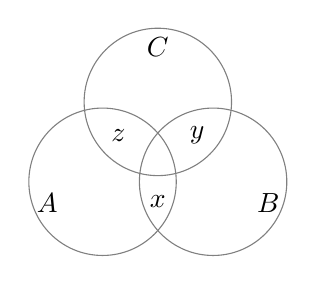
\begin{tikzpicture}[scale=0.78]
\draw[gray] (0,0.75) circle (1.2);
\draw[gray] (-0.9,-0.55) circle (1.2);
\draw[gray] (0.9,-0.55) circle (1.2);
\node at (0,1.65) {$C$};
\node at (-1.8,-0.9) {$A$};
\node at (1.8,-0.9) {$B$};
\node at (-0.64,0.20) {$z$};
\node at (0.64,0.20) {$y$};
\node at (0,-0.88) {$x$};
\end{tikzpicture}
\end{center}
\step{① 集合 $\{1,2,3,4\}$ 中的子集合有 4 个元素，所以从 $1,2,3,4$ 四个元素选 3 个有 $C_4^3=4$ 种方法，将 3 个元素进行全排列有 $P_3^3=3\times2=6$ 种，剩余的一个元素可以分别放入集合 $A$、$B$、$C$，有 3 种，所以此时共有 $3\times4\times6=72$ 种。}
\step{② 集合 $\{1,2,3,4\}$ 中的子集合有 3 个元素，满足集合 $A$、$B$、$C$ 中都只有一个元素。}
\step{所以从 $1,2,3,4$ 四个元素选 3 个有 $C_4^3=4$ 种方法，将 3 个元素进行全排列有 $P_3^3=3\times2=6$ 种，所以此时共有 $4\times6=24$ 种。}
\step{综上，共有 $72+24=96$ 个。}
\solend
\fi

\item 设 $a\in\R$，记 $f(x)=x^2+2x+a$，若关于 $x$ 的不等式 $f(f(x))<0$ 的解集为 $\varnothing$，则 $a$ 的取值范围为 \blankline[4.4em].

\ifanswer
\solbegin
\step{二次函数 $f(x)=x^2+2x+a$ 的开口向上，对称轴为 $x=-1$，所以 $f(x)_{\min}=f(-1)=a-1$，即 $f(x)$ 的值域为 $[a-1,+\infty)$.}
\step{要使不等式 $f(f(x))<0$ 的解集为空集，则 $f(f(x))\geqslant0$ 恒成立，}
\step{所以 $\begin{cases}f(a-1)\geqslant0,\\a-1\geqslant-1,\end{cases}$ 即 $\begin{cases}a^2+a-1\geqslant0,\\a\geqslant0,\end{cases}$}
\step{解得 $a\geqslant\dfrac{\sqrt5-1}{2}$，所以实数 $a$ 的取值范围为 $\left[\dfrac{\sqrt5-1}{2},+\infty\right)$.}
\solend
\fi

\end{enumerate}

\bigsec{二、选择题}

\begin{enumerate}
\setcounter{enumi}{12}

\item 已知关于 $x$ 的不等式 $2x-1>a(x-2)$ 的解集是 $\R$，则数 $a$ 的取值范围是\mbox{（\quad）}

\keepwithprev
A. $a>2$\qquad B. $a=2$

C. $a<2$\qquad D. $a$ 不存在

\ans{$B$}

\item 设 $0<a_1<a_2$，$0<b_1<b_2$，且 $a_1+a_2=b_1+b_2=1$，如果要把 $a_1b_1+a_2b_2$、$a_1b_2+a_2b_1$、$\dfrac12$ 按从小到大的顺序排列，那么排在中间的数是\mbox{（\quad）}

\keepwithprev
A. 一定是 $a_1b_1+a_2b_2$\qquad B. 一定是 $a_1b_2+a_2b_1$

C. 一定是 $\dfrac12$\qquad D. 不能确定，与 $a_1,a_2,b_1,b_2$ 的值有关

\ans{$C$}

\item “$0<a<b$”是“$a-\dfrac1a<b-\dfrac1b$”的\mbox{（\quad）}条件

\keepwithprev
A. 充分不必要\qquad B. 必要不充分

C. 充分必要\qquad D. 既不充分也不必要

\ans{$A$}

\item 在 $n$ 元集合 $S=\{a_1,a_2,\cdots,a_n\}$ 中，设 $x(S)=\dfrac{a_1+a_2+\cdots+a_n}{n}$，若 $S$ 的非空子集 $A$ 满足 $x(A)=x(S)$，则称 $A$ 是集合 $S$ 的一个“平均子集”，并记集合 $S$ 的 $k$ 个“平均子集”的个数为 $f_S(k)$. 已知集合 $S=\{1,2,3,4,5,6,7,8,9\}$，$T=\{-4,-3,-2,-1,0,1,2,3,4\}$，则下列说法错误的是\mbox{（\quad）}

\keepwithprev
A. $f_S(9)=f_T(1)$\qquad B. $f_S(8)=f_T(1)$

C. $f_S(6)=f_T(4)$\qquad D. $f_S(5)=f_T(4)$

\ans{$D$}

\ifanswer
\solbegin
\step{$X(S)=5$，将 $S$ 中的元素分成 5 组 $(1,9)$、$(2,8)$、$(3,7)$、$(4,6)$、$(5)$.}
\step{则 $f_S(1)=C_1^1=1$，$f_S(2)=C_4^1=4$，$f_S(3)=C_1^1C_4^1=4$，$f_S(4)=C_4^2=6$，$f_S(5)=C_1^1C_4^2=6$，同时 $X(T)=0$，将 $T$ 中的元素分成 5 组 $(1,-1)$、$(2,-2)$、$(3,-3)$、$(4,-4)$、$(0)$.}
\step{则 $f_T(1)=C_1^1=1$，$f_T(2)=C_4^1=4$，$f_T(3)=C_1^1C_4^1=4$，$f_T(4)=C_4^2=6$，$f_T(5)=C_1^1C_4^2=6$，$f_T(8)=C_4^4=1$，所以 $f_S(4)=f_S(5)=f_T(4)=6$，故选 D.}
\solend
\fi

\end{enumerate}

\bigsec{三、解答题}

\begin{enumerate}
\setcounter{enumi}{16}

\item 已知集合 $A=\{x\mid x^2-12x+20\leqslant0\}$，$B=\{x\mid2m<x<m+4\}$.

\begin{enumerate}[label=(\arabic*)]
\item 若 $m=3$，求 $A\cup B$；
\item 若 $A\cap B=\varnothing$，求 $m$ 的取值范围.
\end{enumerate}

\ifanswer
\solbegin
\stepm{(1)}{因为 $A=\{x\mid x^2-12x+20\leqslant0\}=\{x\mid2\leqslant x\leqslant10\}$，当 $m=3$ 时，$B=\{x\mid6<x<7\}$，所以 $A\cup B=\{x\mid2\leqslant x\leqslant10\}$.}
\stepm{(2)}{当 $m+4\leqslant2$ 时，$B$ 在 $A$ 的左侧，得 $m\leqslant-2$；当 $2m\geqslant10$ 时，得 $m\geqslant5$；当 $2m\geqslant m+4$ 时，$B=\varnothing$，得 $m\geqslant4$.}
\step{综上，$m\leqslant-2$ 或 $m\geqslant4$.}
\solend
\fi

\item 已知 $a>0$，关于 $x$ 的方程 $\dfrac1{x-2}+\dfrac1{x-1}=\dfrac{\sqrt{ax}}{x^2-3x+2}$ 有且仅有一个实数根，求实数 $a$ 的取值范围.

\ifanswer
\solbegin
\step{由题意得 $x\neq2$，$x\neq1$. 去分母整理得 $2x-3=\sqrt{ax}\geqslant0$，所以 $x\geqslant\dfrac32$，且 $x\neq2$.}
\step{两边平方整理得 $4x^2-(12+a)x+9=0$，判别式 $\Delta=a^2+24a>0$.}
\step{设方程的两个根为 $x_1$、$x_2$，则 $x_1+x_2=\dfrac{12+a}{4}$，$x_1x_2=\dfrac94$.}
\step{当 $0<a<\dfrac12$ 时，方程有一个根在 $\left(\dfrac32,2\right)$ 内，另一个根小于 $\dfrac32$，符合题意；}
\step{当 $a=\dfrac12$ 时，方程的根为 $2$、$\dfrac98$，均不符合题意；}
\step{当 $a>\dfrac12$ 时，方程有一个根大于 $2$，另一个根小于 $\dfrac32$，符合题意。}
\step{综上，实数 $a$ 的取值范围为 $\left(0,\dfrac12\right)\cup\left(\dfrac12,+\infty\right)$.}
\solend
\fi

\item 已知 $a\in\R$，关于 $x$ 的不等式 $ax^2-ax+3>0$ 恒成立.

\begin{enumerate}[label=(\arabic*)]
\item 求实数 $a$ 的取值范围；
\item 在（1）的条件下用反证法证明：三个关于 $x$ 的方程 $x^2+4ax-4a+3=0$，$x^2+(a-1)x+a^2=0$，$x^2+2ax-2a=0$ 中至少有一个方程有实数解.
\end{enumerate}

\ifanswer
\solbegin
\stepm{(1)}{当 $a=0$ 时，$3>0$ 恒成立；当 $a>0$ 时，$\Delta=a^2-12a<0$，解得 $0<a<12$；当 $a<0$ 时，不等式不恒成立。}
\step{综上，$a\in[0,12)$.}
\stepm{(2)}{假设三个方程均无实数解，则}
\step{$\begin{cases}\Delta_1=16a^2+16a-12<0,\\\Delta_2=(a-1)^2-4a^2<0,\\\Delta_3=4a^2+8a<0,\end{cases}$}
\step{解得 $-\dfrac32<a<\dfrac12$，$a<-1$ 或 $a>\dfrac13$，$-2<a<0$.}
\step{由 $a\in[0,12)$，前两个不等式得 $\dfrac13<a<\dfrac12$，第三个不等式得 $-2<a<0$，矛盾。}
\step{所以三个方程中至少有一个方程有实数解。}
\solend
\fi

% 注：原卷条件③按字面未限定 2x∈P_n；若对所有 x∈P_n 都要求 2x∈A，原卷答案 f(4)=4 与之不符。
%     2012 年江苏卷源题将其表述为相对于 P_n 的补集条件；本稿仍照录高一42原文，未替换。
\item 设集合 $P_n=\{1,2,\cdots,n\}$，$n\in\N^*$. 记 $f(n)$ 为同时满足下列条件的集合 $A$ 的个数：

① $A\subseteq P_n$；②若 $x\in A$，则 $2x\notin A$；③若 $x\notin A$，则 $2x\in A$.

\begin{enumerate}[label=(\arabic*)]
\item 求 $f(4)$；
\item 求 $f(n)$ 的解析式（用 $n$ 表示）.
\end{enumerate}

\ifanswer
\solbegin
\stepm{(1)}{当 $n=4$ 时，$P_4=\{1,2,3,4\}$，符合条件的集合 $A$ 为 $\{2\}$、$\{1,4\}$、$\{2,3\}$、$\{1,3,4\}$，故 $f(4)=4$.}
\stepm{(2)}{任取偶数 $x\in P_n$，将 $x$ 除以 2，若商仍为偶数，再除以 2，经过 $k$ 次后商必为奇数，此时商记为 $m$.}
\step{于是 $x=m\cdot2^k$，其中 $m$ 为奇数，$k\in\N^*$.}
\step{由条件得，若 $m\in A$，则 $x\in A\Longleftrightarrow k$ 为偶数；若 $m\notin A$，则 $x\in A\Longleftrightarrow k$ 为奇数。}
\step{因此每个奇数 $m\in P_n$ 是否属于 $A$ 可任意选择，且确定后其所有倍数的归属也唯一确定。}
\step{当 $n$ 为偶数时，$P_n$ 中奇数有 $\dfrac n2$ 个；当 $n$ 为奇数时，$P_n$ 中奇数有 $\dfrac{n+1}{2}$ 个。}
\step{所以 $f(n)=\begin{cases}2^{\frac n2},&n\text{ 为偶数},\\2^{\frac{n+1}{2}},&n\text{ 为奇数} .\end{cases}$}
\solend
\fi

\item 设 $S_n=\{(x_1,x_2,\cdots,x_n)\mid x_i\in\{0,1\},\ i=1,2,\cdots,n\}$（$n$ 为正整数），对任意的 $\alpha=(x_1,x_2,\cdots,x_n)$，$\beta=(y_1,y_2,\cdots,y_n)$，定义 $\alpha\cdot\beta=x_1y_1+x_2y_2+\cdots+x_ny_n$.

\begin{enumerate}[label=(\arabic*)]
\item 当 $n=3$ 时，$\alpha=(1,1,0)$，$\beta=(1,0,1)$，求 $\alpha\cdot\beta$；
\item 当 $n=3$ 时，集合 $A\subseteq S_n$，对任意 $\alpha,\beta\in A$，$\alpha\cdot\beta$ 均为偶数，求 $A$ 中元素个数的最大值；
\item 集合 $A\subseteq S_n$，对任意 $\alpha,\beta\in A$，$\alpha\neq\beta$，均有 $\alpha\cdot\beta\neq0$，求 $A$ 中元素个数的最大值.
\end{enumerate}

\ifanswer
\solbegin
\stepm{(1)}{当 $n=3$ 时，$\alpha\cdot\beta=x_1y_1+x_2y_2+x_3y_3=1\times1+1\times0+0\times1=1$.}
\stepm{(2)}{因为 $\alpha\cdot\beta=x_1y_1+x_2y_2+x_3y_3$ 均为偶数，所以结果为 $0$ 或 $2$.}
\step{当 $\alpha\cdot\beta=0$，则 $A$ 中元素个数最多有 $4$ 个；当 $\alpha\cdot\beta=2$，则 $A$ 中元素个数最多有 $1$ 个。}
\step{综上，$A$ 中元素个数的最大值为 $4$.}
\stepm{(3)}{若 $\alpha=(x_1,x_2,\cdots,x_n)\in A$，令 $\gamma=(1-x_1,1-x_2,\cdots,1-x_n)$，则 $\alpha\cdot\gamma=0$.}
\step{因为 $\alpha\cdot\beta\neq0$，$\alpha\in A$，所以 $\gamma\notin A$.}
\step{因为 $S_n$ 中有 $2^n$ 个元素，所以 $A$ 中元素个数最多有 $\dfrac{2^n}{2}=2^{n-1}$ 个。}
\step{综上，$A$ 中元素个数的最大值为 $2^{n-1}$.}
\solend
\fi

\end{enumerate}

\end{document}
"
% 紧凑版：xelatex "\def\iscompact{1}% 高一42_复旦附中_周末作业4.tex
%   —— 高一上数学“2026-2027 年复旦附中高一上周末作业 4”（试卷版/答案版）
% 试卷版：xelatex 高一42_复旦附中_周末作业4.tex
% 答案版：xelatex "\def\isanswer{1}\input{高一42_复旦附中_周末作业4.tex}"
% 紧凑版：xelatex "\def\iscompact{1}\input{高一42_复旦附中_周末作业4.tex}"
%
% 原始材料：微信公众号“魔都数学加油站”文章，作者破晓，2026-10-01 21:37 发布；
% 文章标题“27学年高一42——2026-2027年上海市复旦附中高一上周末作业4”；
% URL：https://mp.weixin.qq.com/s/nZ8aTd6K9OLS9S4-J-O7lA。
% 正文为 8 张 PNG 页（第 02、08 页 2560×3620，其余六页 4762×6735）。题目、答案及解析均据原图转录。
%
% 卷面标题行印作“2026-2027 年复旦附中高一上周末作业 4”，未印“上海市”；本稿标题照卷面，
% 年份区间按全稿惯例排 en dash。卷面未印副标题，本稿按“知识模块”口径标为“集合与常用逻辑用语、不等式”。
%
% 与原卷的排版差异：
%   ① 原文题号从第 3 题开始，本稿保留原题号；
%   ② 原卷的“一、填空题”“二、选择题”“三、解答题”改排为全稿统一的大节标题；
%   ③ 原卷填空横线统一排为 \blankline[4.4em]；选择题答案统一用 \ans{} 排在选项之后，
%      答案版与试卷版分离；原卷题目下方印出的【答案】、【解析】在答案版中排出；
%   ④ 原卷的粉色斜水印“魔都数学加油站”未录入；第 11 题解析中的三集合示意图以 TikZ 重绘。
%
% 原卷存疑处（照录原文）：
%   ① 第 5 题印出的答案为 $P>Q$，但取 $a=8,b=1$ 即得 $P=1<Q=\sqrt[3]{7}$；本稿照录；
%   ② 第 16 题解析按对称数对计数，印出 f_T(4)=C_4^2=6 并据此“故选 D”；但 T 中还可见
%      {0,1,2,-3} 这类和为 0 的四元子集，原卷的计数及选项结论疑有遗漏，本稿保留原解析和答案；
%   ③ 第 20 题的条件③印作“若 x∉A，则 2x∈A”，未明确限定 2x∈P_n；按此字面读法，f(4)
%      与【解析】列出的四个集合不符，而原题源 2012 年江苏卷明确写补集相对 P_n。
%      本稿照录原卷，不改条件，也不以源题替换；
%   ④ 第 21(2) 题题干未写 α≠β，解析结论为 4；此处照卷面题干与结论录入。
\documentclass[a4paper,11pt]{article}
\usepackage{common}

\begin{document}

\examtitlest[4]{2026--2027 年复旦附中高一上周末作业 4}{集合与常用逻辑用语、不等式}

\bigsec{一、填空题}

\begin{enumerate}
\setcounter{enumi}{2}

\item 若 $-1<x<y<2$，则 $x-y$ 的取值范围为 \blankline[4.4em].

\ifanswer
\solbegin
\step{$(-3,0)$.}
\solend
\fi

\item 已知 $c>d$，若 $ac+bd>bc+ad$，则 $a-b$ 与 $0$ 的大小关系是 \blankline[4.4em].

\ifanswer
\solbegin
\step{$a-b>0$.}
\solend
\fi

\item 已知 $a>b>0$，$P=\sqrt[3]{a}-\sqrt[3]{b}$，$Q=\sqrt[3]{a-b}$，则 $P$、$Q$ 的大小关系是 \blankline[4.4em].

\ifanswer
\solbegin
\step{$P>Q$.}
\solend
\fi

\item 对任意的实数 $x$，不等式 $x+|x-1|\geqslant m$ 恒成立，则实数 $m$ 的取值范围是 \blankline[4.4em].

\ifanswer
\solbegin
\step{令 $f(x)=x+|x-1|=\begin{cases}2x-1,&x\geqslant1,\\1,&x<1.\end{cases}$}
\step{当 $x\geqslant1$ 时，不等式变为 $2x-1\geqslant m$，显然满足题意；}
\step{当 $x<1$ 时，不等式变为 $1\geqslant m$，解得 $m\leqslant1$.}
\step{综上，$m\leqslant1$.}
\solend
\fi

\item 若“存在 $x\in\{x\mid1\leqslant x\leqslant2\}$，使得 $3x+a+1\geqslant0$”是命题，则实数 $a$ 的取值范围是 \blankline[4.4em].

\ifanswer
\solbegin
\step{由题意得 $6+a+1\geqslant0$，所以 $a\geqslant-7$.}
\solend
\fi

\item 已知关于 $x$ 的不等式 $ax-b\leqslant0$ 的解集是 $[2,+\infty)$，则关于 $x$ 的不等式
$ax^2+(3a-b)x-3b<0$ 的解集是 \blankline[4.4em].

\ifanswer
\solbegin
\step{由题意得 $a<0$，且 $\dfrac ba=2$，所以 $b=2a$.}
\step{当 $a<0$ 时，$ax^2+(3a-b)x-3b<0$ 等价于 $x^2+x-6>0$，}
\step{解得 $x\in(-\infty,-3)\cup(2,+\infty)$.}
\solend
\fi

\item 若关于 $x$ 的不等式 $(k^2+4k-5)x^2+4(1-k)x+3>0$ 恒成立，则实数 $k$ 的取值范围是 \blankline[4.4em].

\ifanswer
\solbegin
\step{当 $k=-5$ 时，不等式变为 $24x+3>0$，显然不满足题意，所以 $k\neq-5$.}
\step{当 $k=1$ 时，不等式变为 $3>0$，显然满足题意，所以 $k=1$.}
\step{当 $k^2+4k-5\neq0$ 时，有 $\begin{cases}k^2+4k-5>0,\\\Delta<0,\end{cases}$}
\step{即 $\begin{cases}k^2+4k-5>0,\\4(k-1)(k-19)<0,\end{cases}$，解得 $1<k<19$.}
\step{综上，实数 $k$ 的取值范围是 $[1,19)$.}
\solend
\fi

\item 设 $a\in\R$，集合 $A=\{x\mid x^2-ax+a\leqslant0\}$，若 $A\cap\N\neq\varnothing$，则 $a$ 的取值范围是 \blankline[4.4em].

\ifanswer
\solbegin
\step{$(-\infty,0]\cup[4,+\infty)$.}
\solend
\fi

\item 用 $|S|$ 表示集合 $S$ 中的元素的个数，设 $A$、$B$、$C$ 为集合，称 $(A,B,C)$ 为有序三元组。如果集合 $A$、$B$、$C$ 满足 $|A\cap B|=|B\cap C|=|C\cap A|=1$，且 $|A\cap B\cap C|=0$，则称有序三元组 $(A,B,C)$ 为最小交。由集合 $\{1,2,3,4\}$ 的子集构成的所有有序三元组中，最小交的有序三元组的个数为 \blankline[4.4em].

\ifanswer
\solbegin
\step{设 $A\cap B=\{x\}$，$B\cap C=\{y\}$，$C\cap A=\{z\}$，则 $x,y,z\in\{1,2,3,4\}$，且 $x,y,z$ 互不相同。}
\begin{center}
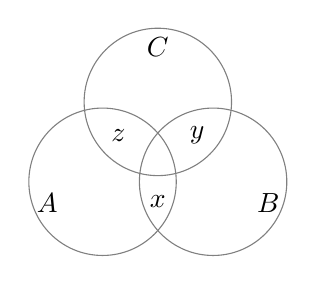
\begin{tikzpicture}[scale=0.78]
\draw[gray] (0,0.75) circle (1.2);
\draw[gray] (-0.9,-0.55) circle (1.2);
\draw[gray] (0.9,-0.55) circle (1.2);
\node at (0,1.65) {$C$};
\node at (-1.8,-0.9) {$A$};
\node at (1.8,-0.9) {$B$};
\node at (-0.64,0.20) {$z$};
\node at (0.64,0.20) {$y$};
\node at (0,-0.88) {$x$};
\end{tikzpicture}
\end{center}
\step{① 集合 $\{1,2,3,4\}$ 中的子集合有 4 个元素，所以从 $1,2,3,4$ 四个元素选 3 个有 $C_4^3=4$ 种方法，将 3 个元素进行全排列有 $P_3^3=3\times2=6$ 种，剩余的一个元素可以分别放入集合 $A$、$B$、$C$，有 3 种，所以此时共有 $3\times4\times6=72$ 种。}
\step{② 集合 $\{1,2,3,4\}$ 中的子集合有 3 个元素，满足集合 $A$、$B$、$C$ 中都只有一个元素。}
\step{所以从 $1,2,3,4$ 四个元素选 3 个有 $C_4^3=4$ 种方法，将 3 个元素进行全排列有 $P_3^3=3\times2=6$ 种，所以此时共有 $4\times6=24$ 种。}
\step{综上，共有 $72+24=96$ 个。}
\solend
\fi

\item 设 $a\in\R$，记 $f(x)=x^2+2x+a$，若关于 $x$ 的不等式 $f(f(x))<0$ 的解集为 $\varnothing$，则 $a$ 的取值范围为 \blankline[4.4em].

\ifanswer
\solbegin
\step{二次函数 $f(x)=x^2+2x+a$ 的开口向上，对称轴为 $x=-1$，所以 $f(x)_{\min}=f(-1)=a-1$，即 $f(x)$ 的值域为 $[a-1,+\infty)$.}
\step{要使不等式 $f(f(x))<0$ 的解集为空集，则 $f(f(x))\geqslant0$ 恒成立，}
\step{所以 $\begin{cases}f(a-1)\geqslant0,\\a-1\geqslant-1,\end{cases}$ 即 $\begin{cases}a^2+a-1\geqslant0,\\a\geqslant0,\end{cases}$}
\step{解得 $a\geqslant\dfrac{\sqrt5-1}{2}$，所以实数 $a$ 的取值范围为 $\left[\dfrac{\sqrt5-1}{2},+\infty\right)$.}
\solend
\fi

\end{enumerate}

\bigsec{二、选择题}

\begin{enumerate}
\setcounter{enumi}{12}

\item 已知关于 $x$ 的不等式 $2x-1>a(x-2)$ 的解集是 $\R$，则数 $a$ 的取值范围是\mbox{（\quad）}

\keepwithprev
A. $a>2$\qquad B. $a=2$

C. $a<2$\qquad D. $a$ 不存在

\ans{$B$}

\item 设 $0<a_1<a_2$，$0<b_1<b_2$，且 $a_1+a_2=b_1+b_2=1$，如果要把 $a_1b_1+a_2b_2$、$a_1b_2+a_2b_1$、$\dfrac12$ 按从小到大的顺序排列，那么排在中间的数是\mbox{（\quad）}

\keepwithprev
A. 一定是 $a_1b_1+a_2b_2$\qquad B. 一定是 $a_1b_2+a_2b_1$

C. 一定是 $\dfrac12$\qquad D. 不能确定，与 $a_1,a_2,b_1,b_2$ 的值有关

\ans{$C$}

\item “$0<a<b$”是“$a-\dfrac1a<b-\dfrac1b$”的\mbox{（\quad）}条件

\keepwithprev
A. 充分不必要\qquad B. 必要不充分

C. 充分必要\qquad D. 既不充分也不必要

\ans{$A$}

\item 在 $n$ 元集合 $S=\{a_1,a_2,\cdots,a_n\}$ 中，设 $x(S)=\dfrac{a_1+a_2+\cdots+a_n}{n}$，若 $S$ 的非空子集 $A$ 满足 $x(A)=x(S)$，则称 $A$ 是集合 $S$ 的一个“平均子集”，并记集合 $S$ 的 $k$ 个“平均子集”的个数为 $f_S(k)$. 已知集合 $S=\{1,2,3,4,5,6,7,8,9\}$，$T=\{-4,-3,-2,-1,0,1,2,3,4\}$，则下列说法错误的是\mbox{（\quad）}

\keepwithprev
A. $f_S(9)=f_T(1)$\qquad B. $f_S(8)=f_T(1)$

C. $f_S(6)=f_T(4)$\qquad D. $f_S(5)=f_T(4)$

\ans{$D$}

\ifanswer
\solbegin
\step{$X(S)=5$，将 $S$ 中的元素分成 5 组 $(1,9)$、$(2,8)$、$(3,7)$、$(4,6)$、$(5)$.}
\step{则 $f_S(1)=C_1^1=1$，$f_S(2)=C_4^1=4$，$f_S(3)=C_1^1C_4^1=4$，$f_S(4)=C_4^2=6$，$f_S(5)=C_1^1C_4^2=6$，同时 $X(T)=0$，将 $T$ 中的元素分成 5 组 $(1,-1)$、$(2,-2)$、$(3,-3)$、$(4,-4)$、$(0)$.}
\step{则 $f_T(1)=C_1^1=1$，$f_T(2)=C_4^1=4$，$f_T(3)=C_1^1C_4^1=4$，$f_T(4)=C_4^2=6$，$f_T(5)=C_1^1C_4^2=6$，$f_T(8)=C_4^4=1$，所以 $f_S(4)=f_S(5)=f_T(4)=6$，故选 D.}
\solend
\fi

\end{enumerate}

\bigsec{三、解答题}

\begin{enumerate}
\setcounter{enumi}{16}

\item 已知集合 $A=\{x\mid x^2-12x+20\leqslant0\}$，$B=\{x\mid2m<x<m+4\}$.

\begin{enumerate}[label=(\arabic*)]
\item 若 $m=3$，求 $A\cup B$；
\item 若 $A\cap B=\varnothing$，求 $m$ 的取值范围.
\end{enumerate}

\ifanswer
\solbegin
\stepm{(1)}{因为 $A=\{x\mid x^2-12x+20\leqslant0\}=\{x\mid2\leqslant x\leqslant10\}$，当 $m=3$ 时，$B=\{x\mid6<x<7\}$，所以 $A\cup B=\{x\mid2\leqslant x\leqslant10\}$.}
\stepm{(2)}{当 $m+4\leqslant2$ 时，$B$ 在 $A$ 的左侧，得 $m\leqslant-2$；当 $2m\geqslant10$ 时，得 $m\geqslant5$；当 $2m\geqslant m+4$ 时，$B=\varnothing$，得 $m\geqslant4$.}
\step{综上，$m\leqslant-2$ 或 $m\geqslant4$.}
\solend
\fi

\item 已知 $a>0$，关于 $x$ 的方程 $\dfrac1{x-2}+\dfrac1{x-1}=\dfrac{\sqrt{ax}}{x^2-3x+2}$ 有且仅有一个实数根，求实数 $a$ 的取值范围.

\ifanswer
\solbegin
\step{由题意得 $x\neq2$，$x\neq1$. 去分母整理得 $2x-3=\sqrt{ax}\geqslant0$，所以 $x\geqslant\dfrac32$，且 $x\neq2$.}
\step{两边平方整理得 $4x^2-(12+a)x+9=0$，判别式 $\Delta=a^2+24a>0$.}
\step{设方程的两个根为 $x_1$、$x_2$，则 $x_1+x_2=\dfrac{12+a}{4}$，$x_1x_2=\dfrac94$.}
\step{当 $0<a<\dfrac12$ 时，方程有一个根在 $\left(\dfrac32,2\right)$ 内，另一个根小于 $\dfrac32$，符合题意；}
\step{当 $a=\dfrac12$ 时，方程的根为 $2$、$\dfrac98$，均不符合题意；}
\step{当 $a>\dfrac12$ 时，方程有一个根大于 $2$，另一个根小于 $\dfrac32$，符合题意。}
\step{综上，实数 $a$ 的取值范围为 $\left(0,\dfrac12\right)\cup\left(\dfrac12,+\infty\right)$.}
\solend
\fi

\item 已知 $a\in\R$，关于 $x$ 的不等式 $ax^2-ax+3>0$ 恒成立.

\begin{enumerate}[label=(\arabic*)]
\item 求实数 $a$ 的取值范围；
\item 在（1）的条件下用反证法证明：三个关于 $x$ 的方程 $x^2+4ax-4a+3=0$，$x^2+(a-1)x+a^2=0$，$x^2+2ax-2a=0$ 中至少有一个方程有实数解.
\end{enumerate}

\ifanswer
\solbegin
\stepm{(1)}{当 $a=0$ 时，$3>0$ 恒成立；当 $a>0$ 时，$\Delta=a^2-12a<0$，解得 $0<a<12$；当 $a<0$ 时，不等式不恒成立。}
\step{综上，$a\in[0,12)$.}
\stepm{(2)}{假设三个方程均无实数解，则}
\step{$\begin{cases}\Delta_1=16a^2+16a-12<0,\\\Delta_2=(a-1)^2-4a^2<0,\\\Delta_3=4a^2+8a<0,\end{cases}$}
\step{解得 $-\dfrac32<a<\dfrac12$，$a<-1$ 或 $a>\dfrac13$，$-2<a<0$.}
\step{由 $a\in[0,12)$，前两个不等式得 $\dfrac13<a<\dfrac12$，第三个不等式得 $-2<a<0$，矛盾。}
\step{所以三个方程中至少有一个方程有实数解。}
\solend
\fi

% 注：原卷条件③按字面未限定 2x∈P_n；若对所有 x∈P_n 都要求 2x∈A，原卷答案 f(4)=4 与之不符。
%     2012 年江苏卷源题将其表述为相对于 P_n 的补集条件；本稿仍照录高一42原文，未替换。
\item 设集合 $P_n=\{1,2,\cdots,n\}$，$n\in\N^*$. 记 $f(n)$ 为同时满足下列条件的集合 $A$ 的个数：

① $A\subseteq P_n$；②若 $x\in A$，则 $2x\notin A$；③若 $x\notin A$，则 $2x\in A$.

\begin{enumerate}[label=(\arabic*)]
\item 求 $f(4)$；
\item 求 $f(n)$ 的解析式（用 $n$ 表示）.
\end{enumerate}

\ifanswer
\solbegin
\stepm{(1)}{当 $n=4$ 时，$P_4=\{1,2,3,4\}$，符合条件的集合 $A$ 为 $\{2\}$、$\{1,4\}$、$\{2,3\}$、$\{1,3,4\}$，故 $f(4)=4$.}
\stepm{(2)}{任取偶数 $x\in P_n$，将 $x$ 除以 2，若商仍为偶数，再除以 2，经过 $k$ 次后商必为奇数，此时商记为 $m$.}
\step{于是 $x=m\cdot2^k$，其中 $m$ 为奇数，$k\in\N^*$.}
\step{由条件得，若 $m\in A$，则 $x\in A\Longleftrightarrow k$ 为偶数；若 $m\notin A$，则 $x\in A\Longleftrightarrow k$ 为奇数。}
\step{因此每个奇数 $m\in P_n$ 是否属于 $A$ 可任意选择，且确定后其所有倍数的归属也唯一确定。}
\step{当 $n$ 为偶数时，$P_n$ 中奇数有 $\dfrac n2$ 个；当 $n$ 为奇数时，$P_n$ 中奇数有 $\dfrac{n+1}{2}$ 个。}
\step{所以 $f(n)=\begin{cases}2^{\frac n2},&n\text{ 为偶数},\\2^{\frac{n+1}{2}},&n\text{ 为奇数} .\end{cases}$}
\solend
\fi

\item 设 $S_n=\{(x_1,x_2,\cdots,x_n)\mid x_i\in\{0,1\},\ i=1,2,\cdots,n\}$（$n$ 为正整数），对任意的 $\alpha=(x_1,x_2,\cdots,x_n)$，$\beta=(y_1,y_2,\cdots,y_n)$，定义 $\alpha\cdot\beta=x_1y_1+x_2y_2+\cdots+x_ny_n$.

\begin{enumerate}[label=(\arabic*)]
\item 当 $n=3$ 时，$\alpha=(1,1,0)$，$\beta=(1,0,1)$，求 $\alpha\cdot\beta$；
\item 当 $n=3$ 时，集合 $A\subseteq S_n$，对任意 $\alpha,\beta\in A$，$\alpha\cdot\beta$ 均为偶数，求 $A$ 中元素个数的最大值；
\item 集合 $A\subseteq S_n$，对任意 $\alpha,\beta\in A$，$\alpha\neq\beta$，均有 $\alpha\cdot\beta\neq0$，求 $A$ 中元素个数的最大值.
\end{enumerate}

\ifanswer
\solbegin
\stepm{(1)}{当 $n=3$ 时，$\alpha\cdot\beta=x_1y_1+x_2y_2+x_3y_3=1\times1+1\times0+0\times1=1$.}
\stepm{(2)}{因为 $\alpha\cdot\beta=x_1y_1+x_2y_2+x_3y_3$ 均为偶数，所以结果为 $0$ 或 $2$.}
\step{当 $\alpha\cdot\beta=0$，则 $A$ 中元素个数最多有 $4$ 个；当 $\alpha\cdot\beta=2$，则 $A$ 中元素个数最多有 $1$ 个。}
\step{综上，$A$ 中元素个数的最大值为 $4$.}
\stepm{(3)}{若 $\alpha=(x_1,x_2,\cdots,x_n)\in A$，令 $\gamma=(1-x_1,1-x_2,\cdots,1-x_n)$，则 $\alpha\cdot\gamma=0$.}
\step{因为 $\alpha\cdot\beta\neq0$，$\alpha\in A$，所以 $\gamma\notin A$.}
\step{因为 $S_n$ 中有 $2^n$ 个元素，所以 $A$ 中元素个数最多有 $\dfrac{2^n}{2}=2^{n-1}$ 个。}
\step{综上，$A$ 中元素个数的最大值为 $2^{n-1}$.}
\solend
\fi

\end{enumerate}

\end{document}
"
%
% 原始材料：微信公众号“魔都数学加油站”文章，作者破晓，2026-10-01 21:37 发布；
% 文章标题“27学年高一42——2026-2027年上海市复旦附中高一上周末作业4”；
% URL：https://mp.weixin.qq.com/s/nZ8aTd6K9OLS9S4-J-O7lA。
% 正文为 8 张 PNG 页（第 02、08 页 2560×3620，其余六页 4762×6735）。题目、答案及解析均据原图转录。
%
% 卷面标题行印作“2026-2027 年复旦附中高一上周末作业 4”，未印“上海市”；本稿标题照卷面，
% 年份区间按全稿惯例排 en dash。卷面未印副标题，本稿按“知识模块”口径标为“集合与常用逻辑用语、不等式”。
%
% 与原卷的排版差异：
%   ① 原文题号从第 3 题开始，本稿保留原题号；
%   ② 原卷的“一、填空题”“二、选择题”“三、解答题”改排为全稿统一的大节标题；
%   ③ 原卷填空横线统一排为 \blankline[4.4em]；选择题答案统一用 \ans{} 排在选项之后，
%      答案版与试卷版分离；原卷题目下方印出的【答案】、【解析】在答案版中排出；
%   ④ 原卷的粉色斜水印“魔都数学加油站”未录入；第 11 题解析中的三集合示意图以 TikZ 重绘。
%
% 原卷存疑处（照录原文）：
%   ① 第 5 题印出的答案为 $P>Q$，但取 $a=8,b=1$ 即得 $P=1<Q=\sqrt[3]{7}$；本稿照录；
%   ② 第 16 题解析按对称数对计数，印出 f_T(4)=C_4^2=6 并据此“故选 D”；但 T 中还可见
%      {0,1,2,-3} 这类和为 0 的四元子集，原卷的计数及选项结论疑有遗漏，本稿保留原解析和答案；
%   ③ 第 20 题的条件③印作“若 x∉A，则 2x∈A”，未明确限定 2x∈P_n；按此字面读法，f(4)
%      与【解析】列出的四个集合不符，而原题源 2012 年江苏卷明确写补集相对 P_n。
%      本稿照录原卷，不改条件，也不以源题替换；
%   ④ 第 21(2) 题题干未写 α≠β，解析结论为 4；此处照卷面题干与结论录入。
\documentclass[a4paper,11pt]{article}
\usepackage{common}

\begin{document}

\examtitlest[4]{2026--2027 年复旦附中高一上周末作业 4}{集合与常用逻辑用语、不等式}

\bigsec{一、填空题}

\begin{enumerate}
\setcounter{enumi}{2}

\item 若 $-1<x<y<2$，则 $x-y$ 的取值范围为 \blankline[4.4em].

\ifanswer
\solbegin
\step{$(-3,0)$.}
\solend
\fi

\item 已知 $c>d$，若 $ac+bd>bc+ad$，则 $a-b$ 与 $0$ 的大小关系是 \blankline[4.4em].

\ifanswer
\solbegin
\step{$a-b>0$.}
\solend
\fi

\item 已知 $a>b>0$，$P=\sqrt[3]{a}-\sqrt[3]{b}$，$Q=\sqrt[3]{a-b}$，则 $P$、$Q$ 的大小关系是 \blankline[4.4em].

\ifanswer
\solbegin
\step{$P>Q$.}
\solend
\fi

\item 对任意的实数 $x$，不等式 $x+|x-1|\geqslant m$ 恒成立，则实数 $m$ 的取值范围是 \blankline[4.4em].

\ifanswer
\solbegin
\step{令 $f(x)=x+|x-1|=\begin{cases}2x-1,&x\geqslant1,\\1,&x<1.\end{cases}$}
\step{当 $x\geqslant1$ 时，不等式变为 $2x-1\geqslant m$，显然满足题意；}
\step{当 $x<1$ 时，不等式变为 $1\geqslant m$，解得 $m\leqslant1$.}
\step{综上，$m\leqslant1$.}
\solend
\fi

\item 若“存在 $x\in\{x\mid1\leqslant x\leqslant2\}$，使得 $3x+a+1\geqslant0$”是命题，则实数 $a$ 的取值范围是 \blankline[4.4em].

\ifanswer
\solbegin
\step{由题意得 $6+a+1\geqslant0$，所以 $a\geqslant-7$.}
\solend
\fi

\item 已知关于 $x$ 的不等式 $ax-b\leqslant0$ 的解集是 $[2,+\infty)$，则关于 $x$ 的不等式
$ax^2+(3a-b)x-3b<0$ 的解集是 \blankline[4.4em].

\ifanswer
\solbegin
\step{由题意得 $a<0$，且 $\dfrac ba=2$，所以 $b=2a$.}
\step{当 $a<0$ 时，$ax^2+(3a-b)x-3b<0$ 等价于 $x^2+x-6>0$，}
\step{解得 $x\in(-\infty,-3)\cup(2,+\infty)$.}
\solend
\fi

\item 若关于 $x$ 的不等式 $(k^2+4k-5)x^2+4(1-k)x+3>0$ 恒成立，则实数 $k$ 的取值范围是 \blankline[4.4em].

\ifanswer
\solbegin
\step{当 $k=-5$ 时，不等式变为 $24x+3>0$，显然不满足题意，所以 $k\neq-5$.}
\step{当 $k=1$ 时，不等式变为 $3>0$，显然满足题意，所以 $k=1$.}
\step{当 $k^2+4k-5\neq0$ 时，有 $\begin{cases}k^2+4k-5>0,\\\Delta<0,\end{cases}$}
\step{即 $\begin{cases}k^2+4k-5>0,\\4(k-1)(k-19)<0,\end{cases}$，解得 $1<k<19$.}
\step{综上，实数 $k$ 的取值范围是 $[1,19)$.}
\solend
\fi

\item 设 $a\in\R$，集合 $A=\{x\mid x^2-ax+a\leqslant0\}$，若 $A\cap\N\neq\varnothing$，则 $a$ 的取值范围是 \blankline[4.4em].

\ifanswer
\solbegin
\step{$(-\infty,0]\cup[4,+\infty)$.}
\solend
\fi

\item 用 $|S|$ 表示集合 $S$ 中的元素的个数，设 $A$、$B$、$C$ 为集合，称 $(A,B,C)$ 为有序三元组。如果集合 $A$、$B$、$C$ 满足 $|A\cap B|=|B\cap C|=|C\cap A|=1$，且 $|A\cap B\cap C|=0$，则称有序三元组 $(A,B,C)$ 为最小交。由集合 $\{1,2,3,4\}$ 的子集构成的所有有序三元组中，最小交的有序三元组的个数为 \blankline[4.4em].

\ifanswer
\solbegin
\step{设 $A\cap B=\{x\}$，$B\cap C=\{y\}$，$C\cap A=\{z\}$，则 $x,y,z\in\{1,2,3,4\}$，且 $x,y,z$ 互不相同。}
\begin{center}
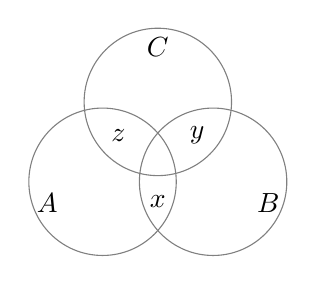
\begin{tikzpicture}[scale=0.78]
\draw[gray] (0,0.75) circle (1.2);
\draw[gray] (-0.9,-0.55) circle (1.2);
\draw[gray] (0.9,-0.55) circle (1.2);
\node at (0,1.65) {$C$};
\node at (-1.8,-0.9) {$A$};
\node at (1.8,-0.9) {$B$};
\node at (-0.64,0.20) {$z$};
\node at (0.64,0.20) {$y$};
\node at (0,-0.88) {$x$};
\end{tikzpicture}
\end{center}
\step{① 集合 $\{1,2,3,4\}$ 中的子集合有 4 个元素，所以从 $1,2,3,4$ 四个元素选 3 个有 $C_4^3=4$ 种方法，将 3 个元素进行全排列有 $P_3^3=3\times2=6$ 种，剩余的一个元素可以分别放入集合 $A$、$B$、$C$，有 3 种，所以此时共有 $3\times4\times6=72$ 种。}
\step{② 集合 $\{1,2,3,4\}$ 中的子集合有 3 个元素，满足集合 $A$、$B$、$C$ 中都只有一个元素。}
\step{所以从 $1,2,3,4$ 四个元素选 3 个有 $C_4^3=4$ 种方法，将 3 个元素进行全排列有 $P_3^3=3\times2=6$ 种，所以此时共有 $4\times6=24$ 种。}
\step{综上，共有 $72+24=96$ 个。}
\solend
\fi

\item 设 $a\in\R$，记 $f(x)=x^2+2x+a$，若关于 $x$ 的不等式 $f(f(x))<0$ 的解集为 $\varnothing$，则 $a$ 的取值范围为 \blankline[4.4em].

\ifanswer
\solbegin
\step{二次函数 $f(x)=x^2+2x+a$ 的开口向上，对称轴为 $x=-1$，所以 $f(x)_{\min}=f(-1)=a-1$，即 $f(x)$ 的值域为 $[a-1,+\infty)$.}
\step{要使不等式 $f(f(x))<0$ 的解集为空集，则 $f(f(x))\geqslant0$ 恒成立，}
\step{所以 $\begin{cases}f(a-1)\geqslant0,\\a-1\geqslant-1,\end{cases}$ 即 $\begin{cases}a^2+a-1\geqslant0,\\a\geqslant0,\end{cases}$}
\step{解得 $a\geqslant\dfrac{\sqrt5-1}{2}$，所以实数 $a$ 的取值范围为 $\left[\dfrac{\sqrt5-1}{2},+\infty\right)$.}
\solend
\fi

\end{enumerate}

\bigsec{二、选择题}

\begin{enumerate}
\setcounter{enumi}{12}

\item 已知关于 $x$ 的不等式 $2x-1>a(x-2)$ 的解集是 $\R$，则数 $a$ 的取值范围是\mbox{（\quad）}

\keepwithprev
A. $a>2$\qquad B. $a=2$

C. $a<2$\qquad D. $a$ 不存在

\ans{$B$}

\item 设 $0<a_1<a_2$，$0<b_1<b_2$，且 $a_1+a_2=b_1+b_2=1$，如果要把 $a_1b_1+a_2b_2$、$a_1b_2+a_2b_1$、$\dfrac12$ 按从小到大的顺序排列，那么排在中间的数是\mbox{（\quad）}

\keepwithprev
A. 一定是 $a_1b_1+a_2b_2$\qquad B. 一定是 $a_1b_2+a_2b_1$

C. 一定是 $\dfrac12$\qquad D. 不能确定，与 $a_1,a_2,b_1,b_2$ 的值有关

\ans{$C$}

\item “$0<a<b$”是“$a-\dfrac1a<b-\dfrac1b$”的\mbox{（\quad）}条件

\keepwithprev
A. 充分不必要\qquad B. 必要不充分

C. 充分必要\qquad D. 既不充分也不必要

\ans{$A$}

\item 在 $n$ 元集合 $S=\{a_1,a_2,\cdots,a_n\}$ 中，设 $x(S)=\dfrac{a_1+a_2+\cdots+a_n}{n}$，若 $S$ 的非空子集 $A$ 满足 $x(A)=x(S)$，则称 $A$ 是集合 $S$ 的一个“平均子集”，并记集合 $S$ 的 $k$ 个“平均子集”的个数为 $f_S(k)$. 已知集合 $S=\{1,2,3,4,5,6,7,8,9\}$，$T=\{-4,-3,-2,-1,0,1,2,3,4\}$，则下列说法错误的是\mbox{（\quad）}

\keepwithprev
A. $f_S(9)=f_T(1)$\qquad B. $f_S(8)=f_T(1)$

C. $f_S(6)=f_T(4)$\qquad D. $f_S(5)=f_T(4)$

\ans{$D$}

\ifanswer
\solbegin
\step{$X(S)=5$，将 $S$ 中的元素分成 5 组 $(1,9)$、$(2,8)$、$(3,7)$、$(4,6)$、$(5)$.}
\step{则 $f_S(1)=C_1^1=1$，$f_S(2)=C_4^1=4$，$f_S(3)=C_1^1C_4^1=4$，$f_S(4)=C_4^2=6$，$f_S(5)=C_1^1C_4^2=6$，同时 $X(T)=0$，将 $T$ 中的元素分成 5 组 $(1,-1)$、$(2,-2)$、$(3,-3)$、$(4,-4)$、$(0)$.}
\step{则 $f_T(1)=C_1^1=1$，$f_T(2)=C_4^1=4$，$f_T(3)=C_1^1C_4^1=4$，$f_T(4)=C_4^2=6$，$f_T(5)=C_1^1C_4^2=6$，$f_T(8)=C_4^4=1$，所以 $f_S(4)=f_S(5)=f_T(4)=6$，故选 D.}
\solend
\fi

\end{enumerate}

\bigsec{三、解答题}

\begin{enumerate}
\setcounter{enumi}{16}

\item 已知集合 $A=\{x\mid x^2-12x+20\leqslant0\}$，$B=\{x\mid2m<x<m+4\}$.

\begin{enumerate}[label=(\arabic*)]
\item 若 $m=3$，求 $A\cup B$；
\item 若 $A\cap B=\varnothing$，求 $m$ 的取值范围.
\end{enumerate}

\ifanswer
\solbegin
\stepm{(1)}{因为 $A=\{x\mid x^2-12x+20\leqslant0\}=\{x\mid2\leqslant x\leqslant10\}$，当 $m=3$ 时，$B=\{x\mid6<x<7\}$，所以 $A\cup B=\{x\mid2\leqslant x\leqslant10\}$.}
\stepm{(2)}{当 $m+4\leqslant2$ 时，$B$ 在 $A$ 的左侧，得 $m\leqslant-2$；当 $2m\geqslant10$ 时，得 $m\geqslant5$；当 $2m\geqslant m+4$ 时，$B=\varnothing$，得 $m\geqslant4$.}
\step{综上，$m\leqslant-2$ 或 $m\geqslant4$.}
\solend
\fi

\item 已知 $a>0$，关于 $x$ 的方程 $\dfrac1{x-2}+\dfrac1{x-1}=\dfrac{\sqrt{ax}}{x^2-3x+2}$ 有且仅有一个实数根，求实数 $a$ 的取值范围.

\ifanswer
\solbegin
\step{由题意得 $x\neq2$，$x\neq1$. 去分母整理得 $2x-3=\sqrt{ax}\geqslant0$，所以 $x\geqslant\dfrac32$，且 $x\neq2$.}
\step{两边平方整理得 $4x^2-(12+a)x+9=0$，判别式 $\Delta=a^2+24a>0$.}
\step{设方程的两个根为 $x_1$、$x_2$，则 $x_1+x_2=\dfrac{12+a}{4}$，$x_1x_2=\dfrac94$.}
\step{当 $0<a<\dfrac12$ 时，方程有一个根在 $\left(\dfrac32,2\right)$ 内，另一个根小于 $\dfrac32$，符合题意；}
\step{当 $a=\dfrac12$ 时，方程的根为 $2$、$\dfrac98$，均不符合题意；}
\step{当 $a>\dfrac12$ 时，方程有一个根大于 $2$，另一个根小于 $\dfrac32$，符合题意。}
\step{综上，实数 $a$ 的取值范围为 $\left(0,\dfrac12\right)\cup\left(\dfrac12,+\infty\right)$.}
\solend
\fi

\item 已知 $a\in\R$，关于 $x$ 的不等式 $ax^2-ax+3>0$ 恒成立.

\begin{enumerate}[label=(\arabic*)]
\item 求实数 $a$ 的取值范围；
\item 在（1）的条件下用反证法证明：三个关于 $x$ 的方程 $x^2+4ax-4a+3=0$，$x^2+(a-1)x+a^2=0$，$x^2+2ax-2a=0$ 中至少有一个方程有实数解.
\end{enumerate}

\ifanswer
\solbegin
\stepm{(1)}{当 $a=0$ 时，$3>0$ 恒成立；当 $a>0$ 时，$\Delta=a^2-12a<0$，解得 $0<a<12$；当 $a<0$ 时，不等式不恒成立。}
\step{综上，$a\in[0,12)$.}
\stepm{(2)}{假设三个方程均无实数解，则}
\step{$\begin{cases}\Delta_1=16a^2+16a-12<0,\\\Delta_2=(a-1)^2-4a^2<0,\\\Delta_3=4a^2+8a<0,\end{cases}$}
\step{解得 $-\dfrac32<a<\dfrac12$，$a<-1$ 或 $a>\dfrac13$，$-2<a<0$.}
\step{由 $a\in[0,12)$，前两个不等式得 $\dfrac13<a<\dfrac12$，第三个不等式得 $-2<a<0$，矛盾。}
\step{所以三个方程中至少有一个方程有实数解。}
\solend
\fi

% 注：原卷条件③按字面未限定 2x∈P_n；若对所有 x∈P_n 都要求 2x∈A，原卷答案 f(4)=4 与之不符。
%     2012 年江苏卷源题将其表述为相对于 P_n 的补集条件；本稿仍照录高一42原文，未替换。
\item 设集合 $P_n=\{1,2,\cdots,n\}$，$n\in\N^*$. 记 $f(n)$ 为同时满足下列条件的集合 $A$ 的个数：

① $A\subseteq P_n$；②若 $x\in A$，则 $2x\notin A$；③若 $x\notin A$，则 $2x\in A$.

\begin{enumerate}[label=(\arabic*)]
\item 求 $f(4)$；
\item 求 $f(n)$ 的解析式（用 $n$ 表示）.
\end{enumerate}

\ifanswer
\solbegin
\stepm{(1)}{当 $n=4$ 时，$P_4=\{1,2,3,4\}$，符合条件的集合 $A$ 为 $\{2\}$、$\{1,4\}$、$\{2,3\}$、$\{1,3,4\}$，故 $f(4)=4$.}
\stepm{(2)}{任取偶数 $x\in P_n$，将 $x$ 除以 2，若商仍为偶数，再除以 2，经过 $k$ 次后商必为奇数，此时商记为 $m$.}
\step{于是 $x=m\cdot2^k$，其中 $m$ 为奇数，$k\in\N^*$.}
\step{由条件得，若 $m\in A$，则 $x\in A\Longleftrightarrow k$ 为偶数；若 $m\notin A$，则 $x\in A\Longleftrightarrow k$ 为奇数。}
\step{因此每个奇数 $m\in P_n$ 是否属于 $A$ 可任意选择，且确定后其所有倍数的归属也唯一确定。}
\step{当 $n$ 为偶数时，$P_n$ 中奇数有 $\dfrac n2$ 个；当 $n$ 为奇数时，$P_n$ 中奇数有 $\dfrac{n+1}{2}$ 个。}
\step{所以 $f(n)=\begin{cases}2^{\frac n2},&n\text{ 为偶数},\\2^{\frac{n+1}{2}},&n\text{ 为奇数} .\end{cases}$}
\solend
\fi

\item 设 $S_n=\{(x_1,x_2,\cdots,x_n)\mid x_i\in\{0,1\},\ i=1,2,\cdots,n\}$（$n$ 为正整数），对任意的 $\alpha=(x_1,x_2,\cdots,x_n)$，$\beta=(y_1,y_2,\cdots,y_n)$，定义 $\alpha\cdot\beta=x_1y_1+x_2y_2+\cdots+x_ny_n$.

\begin{enumerate}[label=(\arabic*)]
\item 当 $n=3$ 时，$\alpha=(1,1,0)$，$\beta=(1,0,1)$，求 $\alpha\cdot\beta$；
\item 当 $n=3$ 时，集合 $A\subseteq S_n$，对任意 $\alpha,\beta\in A$，$\alpha\cdot\beta$ 均为偶数，求 $A$ 中元素个数的最大值；
\item 集合 $A\subseteq S_n$，对任意 $\alpha,\beta\in A$，$\alpha\neq\beta$，均有 $\alpha\cdot\beta\neq0$，求 $A$ 中元素个数的最大值.
\end{enumerate}

\ifanswer
\solbegin
\stepm{(1)}{当 $n=3$ 时，$\alpha\cdot\beta=x_1y_1+x_2y_2+x_3y_3=1\times1+1\times0+0\times1=1$.}
\stepm{(2)}{因为 $\alpha\cdot\beta=x_1y_1+x_2y_2+x_3y_3$ 均为偶数，所以结果为 $0$ 或 $2$.}
\step{当 $\alpha\cdot\beta=0$，则 $A$ 中元素个数最多有 $4$ 个；当 $\alpha\cdot\beta=2$，则 $A$ 中元素个数最多有 $1$ 个。}
\step{综上，$A$ 中元素个数的最大值为 $4$.}
\stepm{(3)}{若 $\alpha=(x_1,x_2,\cdots,x_n)\in A$，令 $\gamma=(1-x_1,1-x_2,\cdots,1-x_n)$，则 $\alpha\cdot\gamma=0$.}
\step{因为 $\alpha\cdot\beta\neq0$，$\alpha\in A$，所以 $\gamma\notin A$.}
\step{因为 $S_n$ 中有 $2^n$ 个元素，所以 $A$ 中元素个数最多有 $\dfrac{2^n}{2}=2^{n-1}$ 个。}
\step{综上，$A$ 中元素个数的最大值为 $2^{n-1}$.}
\solend
\fi

\end{enumerate}

\end{document}
"
%
% 原始材料：微信公众号“魔都数学加油站”文章，作者破晓，2026-10-01 21:37 发布；
% 文章标题“27学年高一42——2026-2027年上海市复旦附中高一上周末作业4”；
% URL：https://mp.weixin.qq.com/s/nZ8aTd6K9OLS9S4-J-O7lA。
% 正文为 8 张 PNG 页（第 02、08 页 2560×3620，其余六页 4762×6735）。题目、答案及解析均据原图转录。
%
% 卷面标题行印作“2026-2027 年复旦附中高一上周末作业 4”，未印“上海市”；本稿标题照卷面，
% 年份区间按全稿惯例排 en dash。卷面未印副标题，本稿按“知识模块”口径标为“集合与常用逻辑用语、不等式”。
%
% 与原卷的排版差异：
%   ① 原文题号从第 3 题开始，本稿保留原题号；
%   ② 原卷的“一、填空题”“二、选择题”“三、解答题”改排为全稿统一的大节标题；
%   ③ 原卷填空横线统一排为 \blankline[4.4em]；选择题答案统一用 \ans{} 排在选项之后，
%      答案版与试卷版分离；原卷题目下方印出的【答案】、【解析】在答案版中排出；
%   ④ 原卷的粉色斜水印“魔都数学加油站”未录入；第 11 题解析中的三集合示意图以 TikZ 重绘。
%
% 原卷存疑处（照录原文）：
%   ① 第 5 题印出的答案为 $P>Q$，但取 $a=8,b=1$ 即得 $P=1<Q=\sqrt[3]{7}$；本稿照录；
%   ② 第 16 题解析按对称数对计数，印出 f_T(4)=C_4^2=6 并据此“故选 D”；但 T 中还可见
%      {0,1,2,-3} 这类和为 0 的四元子集，原卷的计数及选项结论疑有遗漏，本稿保留原解析和答案；
%   ③ 第 20 题的条件③印作“若 x∉A，则 2x∈A”，未明确限定 2x∈P_n；按此字面读法，f(4)
%      与【解析】列出的四个集合不符，而原题源 2012 年江苏卷明确写补集相对 P_n。
%      本稿照录原卷，不改条件，也不以源题替换；
%   ④ 第 21(2) 题题干未写 α≠β，解析结论为 4；此处照卷面题干与结论录入。
\documentclass[a4paper,11pt]{article}
\usepackage{common}

\begin{document}

\examtitlest[4]{2026--2027 年复旦附中高一上周末作业 4}{集合与常用逻辑用语、不等式}

\bigsec{一、填空题}

\begin{enumerate}
\setcounter{enumi}{2}

\item 若 $-1<x<y<2$，则 $x-y$ 的取值范围为 \blankline[4.4em].

\ifanswer
\solbegin
\step{$(-3,0)$.}
\solend
\fi

\item 已知 $c>d$，若 $ac+bd>bc+ad$，则 $a-b$ 与 $0$ 的大小关系是 \blankline[4.4em].

\ifanswer
\solbegin
\step{$a-b>0$.}
\solend
\fi

\item 已知 $a>b>0$，$P=\sqrt[3]{a}-\sqrt[3]{b}$，$Q=\sqrt[3]{a-b}$，则 $P$、$Q$ 的大小关系是 \blankline[4.4em].

\ifanswer
\solbegin
\step{$P>Q$.}
\solend
\fi

\item 对任意的实数 $x$，不等式 $x+|x-1|\geqslant m$ 恒成立，则实数 $m$ 的取值范围是 \blankline[4.4em].

\ifanswer
\solbegin
\step{令 $f(x)=x+|x-1|=\begin{cases}2x-1,&x\geqslant1,\\1,&x<1.\end{cases}$}
\step{当 $x\geqslant1$ 时，不等式变为 $2x-1\geqslant m$，显然满足题意；}
\step{当 $x<1$ 时，不等式变为 $1\geqslant m$，解得 $m\leqslant1$.}
\step{综上，$m\leqslant1$.}
\solend
\fi

\item 若“存在 $x\in\{x\mid1\leqslant x\leqslant2\}$，使得 $3x+a+1\geqslant0$”是命题，则实数 $a$ 的取值范围是 \blankline[4.4em].

\ifanswer
\solbegin
\step{由题意得 $6+a+1\geqslant0$，所以 $a\geqslant-7$.}
\solend
\fi

\item 已知关于 $x$ 的不等式 $ax-b\leqslant0$ 的解集是 $[2,+\infty)$，则关于 $x$ 的不等式
$ax^2+(3a-b)x-3b<0$ 的解集是 \blankline[4.4em].

\ifanswer
\solbegin
\step{由题意得 $a<0$，且 $\dfrac ba=2$，所以 $b=2a$.}
\step{当 $a<0$ 时，$ax^2+(3a-b)x-3b<0$ 等价于 $x^2+x-6>0$，}
\step{解得 $x\in(-\infty,-3)\cup(2,+\infty)$.}
\solend
\fi

\item 若关于 $x$ 的不等式 $(k^2+4k-5)x^2+4(1-k)x+3>0$ 恒成立，则实数 $k$ 的取值范围是 \blankline[4.4em].

\ifanswer
\solbegin
\step{当 $k=-5$ 时，不等式变为 $24x+3>0$，显然不满足题意，所以 $k\neq-5$.}
\step{当 $k=1$ 时，不等式变为 $3>0$，显然满足题意，所以 $k=1$.}
\step{当 $k^2+4k-5\neq0$ 时，有 $\begin{cases}k^2+4k-5>0,\\\Delta<0,\end{cases}$}
\step{即 $\begin{cases}k^2+4k-5>0,\\4(k-1)(k-19)<0,\end{cases}$，解得 $1<k<19$.}
\step{综上，实数 $k$ 的取值范围是 $[1,19)$.}
\solend
\fi

\item 设 $a\in\R$，集合 $A=\{x\mid x^2-ax+a\leqslant0\}$，若 $A\cap\N\neq\varnothing$，则 $a$ 的取值范围是 \blankline[4.4em].

\ifanswer
\solbegin
\step{$(-\infty,0]\cup[4,+\infty)$.}
\solend
\fi

\item 用 $|S|$ 表示集合 $S$ 中的元素的个数，设 $A$、$B$、$C$ 为集合，称 $(A,B,C)$ 为有序三元组。如果集合 $A$、$B$、$C$ 满足 $|A\cap B|=|B\cap C|=|C\cap A|=1$，且 $|A\cap B\cap C|=0$，则称有序三元组 $(A,B,C)$ 为最小交。由集合 $\{1,2,3,4\}$ 的子集构成的所有有序三元组中，最小交的有序三元组的个数为 \blankline[4.4em].

\ifanswer
\solbegin
\step{设 $A\cap B=\{x\}$，$B\cap C=\{y\}$，$C\cap A=\{z\}$，则 $x,y,z\in\{1,2,3,4\}$，且 $x,y,z$ 互不相同。}
\begin{center}
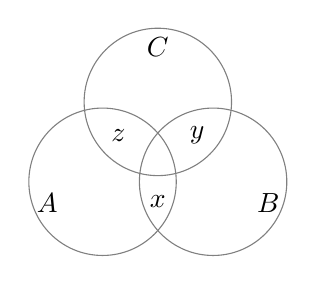
\begin{tikzpicture}[scale=0.78]
\draw[gray] (0,0.75) circle (1.2);
\draw[gray] (-0.9,-0.55) circle (1.2);
\draw[gray] (0.9,-0.55) circle (1.2);
\node at (0,1.65) {$C$};
\node at (-1.8,-0.9) {$A$};
\node at (1.8,-0.9) {$B$};
\node at (-0.64,0.20) {$z$};
\node at (0.64,0.20) {$y$};
\node at (0,-0.88) {$x$};
\end{tikzpicture}
\end{center}
\step{① 集合 $\{1,2,3,4\}$ 中的子集合有 4 个元素，所以从 $1,2,3,4$ 四个元素选 3 个有 $C_4^3=4$ 种方法，将 3 个元素进行全排列有 $P_3^3=3\times2=6$ 种，剩余的一个元素可以分别放入集合 $A$、$B$、$C$，有 3 种，所以此时共有 $3\times4\times6=72$ 种。}
\step{② 集合 $\{1,2,3,4\}$ 中的子集合有 3 个元素，满足集合 $A$、$B$、$C$ 中都只有一个元素。}
\step{所以从 $1,2,3,4$ 四个元素选 3 个有 $C_4^3=4$ 种方法，将 3 个元素进行全排列有 $P_3^3=3\times2=6$ 种，所以此时共有 $4\times6=24$ 种。}
\step{综上，共有 $72+24=96$ 个。}
\solend
\fi

\item 设 $a\in\R$，记 $f(x)=x^2+2x+a$，若关于 $x$ 的不等式 $f(f(x))<0$ 的解集为 $\varnothing$，则 $a$ 的取值范围为 \blankline[4.4em].

\ifanswer
\solbegin
\step{二次函数 $f(x)=x^2+2x+a$ 的开口向上，对称轴为 $x=-1$，所以 $f(x)_{\min}=f(-1)=a-1$，即 $f(x)$ 的值域为 $[a-1,+\infty)$.}
\step{要使不等式 $f(f(x))<0$ 的解集为空集，则 $f(f(x))\geqslant0$ 恒成立，}
\step{所以 $\begin{cases}f(a-1)\geqslant0,\\a-1\geqslant-1,\end{cases}$ 即 $\begin{cases}a^2+a-1\geqslant0,\\a\geqslant0,\end{cases}$}
\step{解得 $a\geqslant\dfrac{\sqrt5-1}{2}$，所以实数 $a$ 的取值范围为 $\left[\dfrac{\sqrt5-1}{2},+\infty\right)$.}
\solend
\fi

\end{enumerate}

\bigsec{二、选择题}

\begin{enumerate}
\setcounter{enumi}{12}

\item 已知关于 $x$ 的不等式 $2x-1>a(x-2)$ 的解集是 $\R$，则数 $a$ 的取值范围是\mbox{（\quad）}

\keepwithprev
A. $a>2$\qquad B. $a=2$

C. $a<2$\qquad D. $a$ 不存在

\ans{$B$}

\item 设 $0<a_1<a_2$，$0<b_1<b_2$，且 $a_1+a_2=b_1+b_2=1$，如果要把 $a_1b_1+a_2b_2$、$a_1b_2+a_2b_1$、$\dfrac12$ 按从小到大的顺序排列，那么排在中间的数是\mbox{（\quad）}

\keepwithprev
A. 一定是 $a_1b_1+a_2b_2$\qquad B. 一定是 $a_1b_2+a_2b_1$

C. 一定是 $\dfrac12$\qquad D. 不能确定，与 $a_1,a_2,b_1,b_2$ 的值有关

\ans{$C$}

\item “$0<a<b$”是“$a-\dfrac1a<b-\dfrac1b$”的\mbox{（\quad）}条件

\keepwithprev
A. 充分不必要\qquad B. 必要不充分

C. 充分必要\qquad D. 既不充分也不必要

\ans{$A$}

\item 在 $n$ 元集合 $S=\{a_1,a_2,\cdots,a_n\}$ 中，设 $x(S)=\dfrac{a_1+a_2+\cdots+a_n}{n}$，若 $S$ 的非空子集 $A$ 满足 $x(A)=x(S)$，则称 $A$ 是集合 $S$ 的一个“平均子集”，并记集合 $S$ 的 $k$ 个“平均子集”的个数为 $f_S(k)$. 已知集合 $S=\{1,2,3,4,5,6,7,8,9\}$，$T=\{-4,-3,-2,-1,0,1,2,3,4\}$，则下列说法错误的是\mbox{（\quad）}

\keepwithprev
A. $f_S(9)=f_T(1)$\qquad B. $f_S(8)=f_T(1)$

C. $f_S(6)=f_T(4)$\qquad D. $f_S(5)=f_T(4)$

\ans{$D$}

\ifanswer
\solbegin
\step{$X(S)=5$，将 $S$ 中的元素分成 5 组 $(1,9)$、$(2,8)$、$(3,7)$、$(4,6)$、$(5)$.}
\step{则 $f_S(1)=C_1^1=1$，$f_S(2)=C_4^1=4$，$f_S(3)=C_1^1C_4^1=4$，$f_S(4)=C_4^2=6$，$f_S(5)=C_1^1C_4^2=6$，同时 $X(T)=0$，将 $T$ 中的元素分成 5 组 $(1,-1)$、$(2,-2)$、$(3,-3)$、$(4,-4)$、$(0)$.}
\step{则 $f_T(1)=C_1^1=1$，$f_T(2)=C_4^1=4$，$f_T(3)=C_1^1C_4^1=4$，$f_T(4)=C_4^2=6$，$f_T(5)=C_1^1C_4^2=6$，$f_T(8)=C_4^4=1$，所以 $f_S(4)=f_S(5)=f_T(4)=6$，故选 D.}
\solend
\fi

\end{enumerate}

\bigsec{三、解答题}

\begin{enumerate}
\setcounter{enumi}{16}

\item 已知集合 $A=\{x\mid x^2-12x+20\leqslant0\}$，$B=\{x\mid2m<x<m+4\}$.

\begin{enumerate}[label=(\arabic*)]
\item 若 $m=3$，求 $A\cup B$；
\item 若 $A\cap B=\varnothing$，求 $m$ 的取值范围.
\end{enumerate}

\ifanswer
\solbegin
\stepm{(1)}{因为 $A=\{x\mid x^2-12x+20\leqslant0\}=\{x\mid2\leqslant x\leqslant10\}$，当 $m=3$ 时，$B=\{x\mid6<x<7\}$，所以 $A\cup B=\{x\mid2\leqslant x\leqslant10\}$.}
\stepm{(2)}{当 $m+4\leqslant2$ 时，$B$ 在 $A$ 的左侧，得 $m\leqslant-2$；当 $2m\geqslant10$ 时，得 $m\geqslant5$；当 $2m\geqslant m+4$ 时，$B=\varnothing$，得 $m\geqslant4$.}
\step{综上，$m\leqslant-2$ 或 $m\geqslant4$.}
\solend
\fi

\item 已知 $a>0$，关于 $x$ 的方程 $\dfrac1{x-2}+\dfrac1{x-1}=\dfrac{\sqrt{ax}}{x^2-3x+2}$ 有且仅有一个实数根，求实数 $a$ 的取值范围.

\ifanswer
\solbegin
\step{由题意得 $x\neq2$，$x\neq1$. 去分母整理得 $2x-3=\sqrt{ax}\geqslant0$，所以 $x\geqslant\dfrac32$，且 $x\neq2$.}
\step{两边平方整理得 $4x^2-(12+a)x+9=0$，判别式 $\Delta=a^2+24a>0$.}
\step{设方程的两个根为 $x_1$、$x_2$，则 $x_1+x_2=\dfrac{12+a}{4}$，$x_1x_2=\dfrac94$.}
\step{当 $0<a<\dfrac12$ 时，方程有一个根在 $\left(\dfrac32,2\right)$ 内，另一个根小于 $\dfrac32$，符合题意；}
\step{当 $a=\dfrac12$ 时，方程的根为 $2$、$\dfrac98$，均不符合题意；}
\step{当 $a>\dfrac12$ 时，方程有一个根大于 $2$，另一个根小于 $\dfrac32$，符合题意。}
\step{综上，实数 $a$ 的取值范围为 $\left(0,\dfrac12\right)\cup\left(\dfrac12,+\infty\right)$.}
\solend
\fi

\item 已知 $a\in\R$，关于 $x$ 的不等式 $ax^2-ax+3>0$ 恒成立.

\begin{enumerate}[label=(\arabic*)]
\item 求实数 $a$ 的取值范围；
\item 在（1）的条件下用反证法证明：三个关于 $x$ 的方程 $x^2+4ax-4a+3=0$，$x^2+(a-1)x+a^2=0$，$x^2+2ax-2a=0$ 中至少有一个方程有实数解.
\end{enumerate}

\ifanswer
\solbegin
\stepm{(1)}{当 $a=0$ 时，$3>0$ 恒成立；当 $a>0$ 时，$\Delta=a^2-12a<0$，解得 $0<a<12$；当 $a<0$ 时，不等式不恒成立。}
\step{综上，$a\in[0,12)$.}
\stepm{(2)}{假设三个方程均无实数解，则}
\step{$\begin{cases}\Delta_1=16a^2+16a-12<0,\\\Delta_2=(a-1)^2-4a^2<0,\\\Delta_3=4a^2+8a<0,\end{cases}$}
\step{解得 $-\dfrac32<a<\dfrac12$，$a<-1$ 或 $a>\dfrac13$，$-2<a<0$.}
\step{由 $a\in[0,12)$，前两个不等式得 $\dfrac13<a<\dfrac12$，第三个不等式得 $-2<a<0$，矛盾。}
\step{所以三个方程中至少有一个方程有实数解。}
\solend
\fi

% 注：原卷条件③按字面未限定 2x∈P_n；若对所有 x∈P_n 都要求 2x∈A，原卷答案 f(4)=4 与之不符。
%     2012 年江苏卷源题将其表述为相对于 P_n 的补集条件；本稿仍照录高一42原文，未替换。
\item 设集合 $P_n=\{1,2,\cdots,n\}$，$n\in\N^*$. 记 $f(n)$ 为同时满足下列条件的集合 $A$ 的个数：

① $A\subseteq P_n$；②若 $x\in A$，则 $2x\notin A$；③若 $x\notin A$，则 $2x\in A$.

\begin{enumerate}[label=(\arabic*)]
\item 求 $f(4)$；
\item 求 $f(n)$ 的解析式（用 $n$ 表示）.
\end{enumerate}

\ifanswer
\solbegin
\stepm{(1)}{当 $n=4$ 时，$P_4=\{1,2,3,4\}$，符合条件的集合 $A$ 为 $\{2\}$、$\{1,4\}$、$\{2,3\}$、$\{1,3,4\}$，故 $f(4)=4$.}
\stepm{(2)}{任取偶数 $x\in P_n$，将 $x$ 除以 2，若商仍为偶数，再除以 2，经过 $k$ 次后商必为奇数，此时商记为 $m$.}
\step{于是 $x=m\cdot2^k$，其中 $m$ 为奇数，$k\in\N^*$.}
\step{由条件得，若 $m\in A$，则 $x\in A\Longleftrightarrow k$ 为偶数；若 $m\notin A$，则 $x\in A\Longleftrightarrow k$ 为奇数。}
\step{因此每个奇数 $m\in P_n$ 是否属于 $A$ 可任意选择，且确定后其所有倍数的归属也唯一确定。}
\step{当 $n$ 为偶数时，$P_n$ 中奇数有 $\dfrac n2$ 个；当 $n$ 为奇数时，$P_n$ 中奇数有 $\dfrac{n+1}{2}$ 个。}
\step{所以 $f(n)=\begin{cases}2^{\frac n2},&n\text{ 为偶数},\\2^{\frac{n+1}{2}},&n\text{ 为奇数} .\end{cases}$}
\solend
\fi

\item 设 $S_n=\{(x_1,x_2,\cdots,x_n)\mid x_i\in\{0,1\},\ i=1,2,\cdots,n\}$（$n$ 为正整数），对任意的 $\alpha=(x_1,x_2,\cdots,x_n)$，$\beta=(y_1,y_2,\cdots,y_n)$，定义 $\alpha\cdot\beta=x_1y_1+x_2y_2+\cdots+x_ny_n$.

\begin{enumerate}[label=(\arabic*)]
\item 当 $n=3$ 时，$\alpha=(1,1,0)$，$\beta=(1,0,1)$，求 $\alpha\cdot\beta$；
\item 当 $n=3$ 时，集合 $A\subseteq S_n$，对任意 $\alpha,\beta\in A$，$\alpha\cdot\beta$ 均为偶数，求 $A$ 中元素个数的最大值；
\item 集合 $A\subseteq S_n$，对任意 $\alpha,\beta\in A$，$\alpha\neq\beta$，均有 $\alpha\cdot\beta\neq0$，求 $A$ 中元素个数的最大值.
\end{enumerate}

\ifanswer
\solbegin
\stepm{(1)}{当 $n=3$ 时，$\alpha\cdot\beta=x_1y_1+x_2y_2+x_3y_3=1\times1+1\times0+0\times1=1$.}
\stepm{(2)}{因为 $\alpha\cdot\beta=x_1y_1+x_2y_2+x_3y_3$ 均为偶数，所以结果为 $0$ 或 $2$.}
\step{当 $\alpha\cdot\beta=0$，则 $A$ 中元素个数最多有 $4$ 个；当 $\alpha\cdot\beta=2$，则 $A$ 中元素个数最多有 $1$ 个。}
\step{综上，$A$ 中元素个数的最大值为 $4$.}
\stepm{(3)}{若 $\alpha=(x_1,x_2,\cdots,x_n)\in A$，令 $\gamma=(1-x_1,1-x_2,\cdots,1-x_n)$，则 $\alpha\cdot\gamma=0$.}
\step{因为 $\alpha\cdot\beta\neq0$，$\alpha\in A$，所以 $\gamma\notin A$.}
\step{因为 $S_n$ 中有 $2^n$ 个元素，所以 $A$ 中元素个数最多有 $\dfrac{2^n}{2}=2^{n-1}$ 个。}
\step{综上，$A$ 中元素个数的最大值为 $2^{n-1}$.}
\solend
\fi

\end{enumerate}

\end{document}
"
%
% 原始材料：微信公众号“魔都数学加油站”文章，作者破晓，2026-10-01 21:37 发布；
% 文章标题“27学年高一42——2026-2027年上海市复旦附中高一上周末作业4”；
% URL：https://mp.weixin.qq.com/s/nZ8aTd6K9OLS9S4-J-O7lA。
% 正文为 8 张 PNG 页（第 02、08 页 2560×3620，其余六页 4762×6735）。题目、答案及解析均据原图转录。
%
% 卷面标题行印作“2026-2027 年复旦附中高一上周末作业 4”，未印“上海市”；本稿标题照卷面，
% 年份区间按全稿惯例排 en dash。卷面未印副标题，本稿按“知识模块”口径标为“集合与常用逻辑用语、不等式”。
%
% 与原卷的排版差异：
%   ① 原文题号从第 3 题开始，本稿保留原题号；
%   ② 原卷的“一、填空题”“二、选择题”“三、解答题”改排为全稿统一的大节标题；
%   ③ 原卷填空横线统一排为 \blankline[4.4em]；选择题答案统一用 \ans{} 排在选项之后，
%      答案版与试卷版分离；原卷题目下方印出的【答案】、【解析】在答案版中排出；
%   ④ 原卷的粉色斜水印“魔都数学加油站”未录入；第 11 题解析中的三集合示意图以 TikZ 重绘。
%
% 原卷存疑处（照录原文）：
%   ① 第 5 题印出的答案为 $P>Q$，但取 $a=8,b=1$ 即得 $P=1<Q=\sqrt[3]{7}$；本稿照录；
%   ② 第 16 题解析按对称数对计数，印出 f_T(4)=C_4^2=6 并据此“故选 D”；但 T 中还可见
%      {0,1,2,-3} 这类和为 0 的四元子集，原卷的计数及选项结论疑有遗漏，本稿保留原解析和答案；
%   ③ 第 20 题的条件③印作“若 x∉A，则 2x∈A”，未明确限定 2x∈P_n；按此字面读法，f(4)
%      与【解析】列出的四个集合不符，而原题源 2012 年江苏卷明确写补集相对 P_n。
%      本稿照录原卷，不改条件，也不以源题替换；
%   ④ 第 21(2) 题题干未写 α≠β，解析结论为 4；此处照卷面题干与结论录入。
\documentclass[a4paper,11pt]{article}
\usepackage{common}

\begin{document}

\examtitlest[4]{2026--2027 年复旦附中高一上周末作业 4}{集合与常用逻辑用语、不等式}

\bigsec{一、填空题}

\begin{enumerate}
\setcounter{enumi}{2}

\item 若 $-1<x<y<2$，则 $x-y$ 的取值范围为 \blankline[4.4em].

\ifanswer
\solbegin
\step{$(-3,0)$.}
\solend
\fi

\item 已知 $c>d$，若 $ac+bd>bc+ad$，则 $a-b$ 与 $0$ 的大小关系是 \blankline[4.4em].

\ifanswer
\solbegin
\step{$a-b>0$.}
\solend
\fi

\item 已知 $a>b>0$，$P=\sqrt[3]{a}-\sqrt[3]{b}$，$Q=\sqrt[3]{a-b}$，则 $P$、$Q$ 的大小关系是 \blankline[4.4em].

\ifanswer
\solbegin
\step{$P>Q$.}
\solend
\fi

\item 对任意的实数 $x$，不等式 $x+|x-1|\geqslant m$ 恒成立，则实数 $m$ 的取值范围是 \blankline[4.4em].

\ifanswer
\solbegin
\step{令 $f(x)=x+|x-1|=\begin{cases}2x-1,&x\geqslant1,\\1,&x<1.\end{cases}$}
\step{当 $x\geqslant1$ 时，不等式变为 $2x-1\geqslant m$，显然满足题意；}
\step{当 $x<1$ 时，不等式变为 $1\geqslant m$，解得 $m\leqslant1$.}
\step{综上，$m\leqslant1$.}
\solend
\fi

\item 若“存在 $x\in\{x\mid1\leqslant x\leqslant2\}$，使得 $3x+a+1\geqslant0$”是命题，则实数 $a$ 的取值范围是 \blankline[4.4em].

\ifanswer
\solbegin
\step{由题意得 $6+a+1\geqslant0$，所以 $a\geqslant-7$.}
\solend
\fi

\item 已知关于 $x$ 的不等式 $ax-b\leqslant0$ 的解集是 $[2,+\infty)$，则关于 $x$ 的不等式
$ax^2+(3a-b)x-3b<0$ 的解集是 \blankline[4.4em].

\ifanswer
\solbegin
\step{由题意得 $a<0$，且 $\dfrac ba=2$，所以 $b=2a$.}
\step{当 $a<0$ 时，$ax^2+(3a-b)x-3b<0$ 等价于 $x^2+x-6>0$，}
\step{解得 $x\in(-\infty,-3)\cup(2,+\infty)$.}
\solend
\fi

\item 若关于 $x$ 的不等式 $(k^2+4k-5)x^2+4(1-k)x+3>0$ 恒成立，则实数 $k$ 的取值范围是 \blankline[4.4em].

\ifanswer
\solbegin
\step{当 $k=-5$ 时，不等式变为 $24x+3>0$，显然不满足题意，所以 $k\neq-5$.}
\step{当 $k=1$ 时，不等式变为 $3>0$，显然满足题意，所以 $k=1$.}
\step{当 $k^2+4k-5\neq0$ 时，有 $\begin{cases}k^2+4k-5>0,\\\Delta<0,\end{cases}$}
\step{即 $\begin{cases}k^2+4k-5>0,\\4(k-1)(k-19)<0,\end{cases}$，解得 $1<k<19$.}
\step{综上，实数 $k$ 的取值范围是 $[1,19)$.}
\solend
\fi

\item 设 $a\in\R$，集合 $A=\{x\mid x^2-ax+a\leqslant0\}$，若 $A\cap\N\neq\varnothing$，则 $a$ 的取值范围是 \blankline[4.4em].

\ifanswer
\solbegin
\step{$(-\infty,0]\cup[4,+\infty)$.}
\solend
\fi

\item 用 $|S|$ 表示集合 $S$ 中的元素的个数，设 $A$、$B$、$C$ 为集合，称 $(A,B,C)$ 为有序三元组。如果集合 $A$、$B$、$C$ 满足 $|A\cap B|=|B\cap C|=|C\cap A|=1$，且 $|A\cap B\cap C|=0$，则称有序三元组 $(A,B,C)$ 为最小交。由集合 $\{1,2,3,4\}$ 的子集构成的所有有序三元组中，最小交的有序三元组的个数为 \blankline[4.4em].

\ifanswer
\solbegin
\step{设 $A\cap B=\{x\}$，$B\cap C=\{y\}$，$C\cap A=\{z\}$，则 $x,y,z\in\{1,2,3,4\}$，且 $x,y,z$ 互不相同。}
\begin{center}
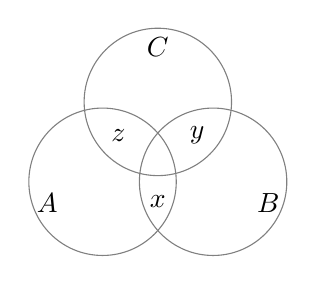
\begin{tikzpicture}[scale=0.78]
\draw[gray] (0,0.75) circle (1.2);
\draw[gray] (-0.9,-0.55) circle (1.2);
\draw[gray] (0.9,-0.55) circle (1.2);
\node at (0,1.65) {$C$};
\node at (-1.8,-0.9) {$A$};
\node at (1.8,-0.9) {$B$};
\node at (-0.64,0.20) {$z$};
\node at (0.64,0.20) {$y$};
\node at (0,-0.88) {$x$};
\end{tikzpicture}
\end{center}
\step{① 集合 $\{1,2,3,4\}$ 中的子集合有 4 个元素，所以从 $1,2,3,4$ 四个元素选 3 个有 $C_4^3=4$ 种方法，将 3 个元素进行全排列有 $P_3^3=3\times2=6$ 种，剩余的一个元素可以分别放入集合 $A$、$B$、$C$，有 3 种，所以此时共有 $3\times4\times6=72$ 种。}
\step{② 集合 $\{1,2,3,4\}$ 中的子集合有 3 个元素，满足集合 $A$、$B$、$C$ 中都只有一个元素。}
\step{所以从 $1,2,3,4$ 四个元素选 3 个有 $C_4^3=4$ 种方法，将 3 个元素进行全排列有 $P_3^3=3\times2=6$ 种，所以此时共有 $4\times6=24$ 种。}
\step{综上，共有 $72+24=96$ 个。}
\solend
\fi

\item 设 $a\in\R$，记 $f(x)=x^2+2x+a$，若关于 $x$ 的不等式 $f(f(x))<0$ 的解集为 $\varnothing$，则 $a$ 的取值范围为 \blankline[4.4em].

\ifanswer
\solbegin
\step{二次函数 $f(x)=x^2+2x+a$ 的开口向上，对称轴为 $x=-1$，所以 $f(x)_{\min}=f(-1)=a-1$，即 $f(x)$ 的值域为 $[a-1,+\infty)$.}
\step{要使不等式 $f(f(x))<0$ 的解集为空集，则 $f(f(x))\geqslant0$ 恒成立，}
\step{所以 $\begin{cases}f(a-1)\geqslant0,\\a-1\geqslant-1,\end{cases}$ 即 $\begin{cases}a^2+a-1\geqslant0,\\a\geqslant0,\end{cases}$}
\step{解得 $a\geqslant\dfrac{\sqrt5-1}{2}$，所以实数 $a$ 的取值范围为 $\left[\dfrac{\sqrt5-1}{2},+\infty\right)$.}
\solend
\fi

\end{enumerate}

\bigsec{二、选择题}

\begin{enumerate}
\setcounter{enumi}{12}

\item 已知关于 $x$ 的不等式 $2x-1>a(x-2)$ 的解集是 $\R$，则数 $a$ 的取值范围是\mbox{（\quad）}

\keepwithprev
A. $a>2$\qquad B. $a=2$

C. $a<2$\qquad D. $a$ 不存在

\ans{$B$}

\item 设 $0<a_1<a_2$，$0<b_1<b_2$，且 $a_1+a_2=b_1+b_2=1$，如果要把 $a_1b_1+a_2b_2$、$a_1b_2+a_2b_1$、$\dfrac12$ 按从小到大的顺序排列，那么排在中间的数是\mbox{（\quad）}

\keepwithprev
A. 一定是 $a_1b_1+a_2b_2$\qquad B. 一定是 $a_1b_2+a_2b_1$

C. 一定是 $\dfrac12$\qquad D. 不能确定，与 $a_1,a_2,b_1,b_2$ 的值有关

\ans{$C$}

\item “$0<a<b$”是“$a-\dfrac1a<b-\dfrac1b$”的\mbox{（\quad）}条件

\keepwithprev
A. 充分不必要\qquad B. 必要不充分

C. 充分必要\qquad D. 既不充分也不必要

\ans{$A$}

\item 在 $n$ 元集合 $S=\{a_1,a_2,\cdots,a_n\}$ 中，设 $x(S)=\dfrac{a_1+a_2+\cdots+a_n}{n}$，若 $S$ 的非空子集 $A$ 满足 $x(A)=x(S)$，则称 $A$ 是集合 $S$ 的一个“平均子集”，并记集合 $S$ 的 $k$ 个“平均子集”的个数为 $f_S(k)$. 已知集合 $S=\{1,2,3,4,5,6,7,8,9\}$，$T=\{-4,-3,-2,-1,0,1,2,3,4\}$，则下列说法错误的是\mbox{（\quad）}

\keepwithprev
A. $f_S(9)=f_T(1)$\qquad B. $f_S(8)=f_T(1)$

C. $f_S(6)=f_T(4)$\qquad D. $f_S(5)=f_T(4)$

\ans{$D$}

\ifanswer
\solbegin
\step{$X(S)=5$，将 $S$ 中的元素分成 5 组 $(1,9)$、$(2,8)$、$(3,7)$、$(4,6)$、$(5)$.}
\step{则 $f_S(1)=C_1^1=1$，$f_S(2)=C_4^1=4$，$f_S(3)=C_1^1C_4^1=4$，$f_S(4)=C_4^2=6$，$f_S(5)=C_1^1C_4^2=6$，同时 $X(T)=0$，将 $T$ 中的元素分成 5 组 $(1,-1)$、$(2,-2)$、$(3,-3)$、$(4,-4)$、$(0)$.}
\step{则 $f_T(1)=C_1^1=1$，$f_T(2)=C_4^1=4$，$f_T(3)=C_1^1C_4^1=4$，$f_T(4)=C_4^2=6$，$f_T(5)=C_1^1C_4^2=6$，$f_T(8)=C_4^4=1$，所以 $f_S(4)=f_S(5)=f_T(4)=6$，故选 D.}
\solend
\fi

\end{enumerate}

\bigsec{三、解答题}

\begin{enumerate}
\setcounter{enumi}{16}

\item 已知集合 $A=\{x\mid x^2-12x+20\leqslant0\}$，$B=\{x\mid2m<x<m+4\}$.

\begin{enumerate}[label=(\arabic*)]
\item 若 $m=3$，求 $A\cup B$；
\item 若 $A\cap B=\varnothing$，求 $m$ 的取值范围.
\end{enumerate}

\ifanswer
\solbegin
\stepm{(1)}{因为 $A=\{x\mid x^2-12x+20\leqslant0\}=\{x\mid2\leqslant x\leqslant10\}$，当 $m=3$ 时，$B=\{x\mid6<x<7\}$，所以 $A\cup B=\{x\mid2\leqslant x\leqslant10\}$.}
\stepm{(2)}{当 $m+4\leqslant2$ 时，$B$ 在 $A$ 的左侧，得 $m\leqslant-2$；当 $2m\geqslant10$ 时，得 $m\geqslant5$；当 $2m\geqslant m+4$ 时，$B=\varnothing$，得 $m\geqslant4$.}
\step{综上，$m\leqslant-2$ 或 $m\geqslant4$.}
\solend
\fi

\item 已知 $a>0$，关于 $x$ 的方程 $\dfrac1{x-2}+\dfrac1{x-1}=\dfrac{\sqrt{ax}}{x^2-3x+2}$ 有且仅有一个实数根，求实数 $a$ 的取值范围.

\ifanswer
\solbegin
\step{由题意得 $x\neq2$，$x\neq1$. 去分母整理得 $2x-3=\sqrt{ax}\geqslant0$，所以 $x\geqslant\dfrac32$，且 $x\neq2$.}
\step{两边平方整理得 $4x^2-(12+a)x+9=0$，判别式 $\Delta=a^2+24a>0$.}
\step{设方程的两个根为 $x_1$、$x_2$，则 $x_1+x_2=\dfrac{12+a}{4}$，$x_1x_2=\dfrac94$.}
\step{当 $0<a<\dfrac12$ 时，方程有一个根在 $\left(\dfrac32,2\right)$ 内，另一个根小于 $\dfrac32$，符合题意；}
\step{当 $a=\dfrac12$ 时，方程的根为 $2$、$\dfrac98$，均不符合题意；}
\step{当 $a>\dfrac12$ 时，方程有一个根大于 $2$，另一个根小于 $\dfrac32$，符合题意。}
\step{综上，实数 $a$ 的取值范围为 $\left(0,\dfrac12\right)\cup\left(\dfrac12,+\infty\right)$.}
\solend
\fi

\item 已知 $a\in\R$，关于 $x$ 的不等式 $ax^2-ax+3>0$ 恒成立.

\begin{enumerate}[label=(\arabic*)]
\item 求实数 $a$ 的取值范围；
\item 在（1）的条件下用反证法证明：三个关于 $x$ 的方程 $x^2+4ax-4a+3=0$，$x^2+(a-1)x+a^2=0$，$x^2+2ax-2a=0$ 中至少有一个方程有实数解.
\end{enumerate}

\ifanswer
\solbegin
\stepm{(1)}{当 $a=0$ 时，$3>0$ 恒成立；当 $a>0$ 时，$\Delta=a^2-12a<0$，解得 $0<a<12$；当 $a<0$ 时，不等式不恒成立。}
\step{综上，$a\in[0,12)$.}
\stepm{(2)}{假设三个方程均无实数解，则}
\step{$\begin{cases}\Delta_1=16a^2+16a-12<0,\\\Delta_2=(a-1)^2-4a^2<0,\\\Delta_3=4a^2+8a<0,\end{cases}$}
\step{解得 $-\dfrac32<a<\dfrac12$，$a<-1$ 或 $a>\dfrac13$，$-2<a<0$.}
\step{由 $a\in[0,12)$，前两个不等式得 $\dfrac13<a<\dfrac12$，第三个不等式得 $-2<a<0$，矛盾。}
\step{所以三个方程中至少有一个方程有实数解。}
\solend
\fi

% 注：原卷条件③按字面未限定 2x∈P_n；若对所有 x∈P_n 都要求 2x∈A，原卷答案 f(4)=4 与之不符。
%     2012 年江苏卷源题将其表述为相对于 P_n 的补集条件；本稿仍照录高一42原文，未替换。
\item 设集合 $P_n=\{1,2,\cdots,n\}$，$n\in\N^*$. 记 $f(n)$ 为同时满足下列条件的集合 $A$ 的个数：

① $A\subseteq P_n$；②若 $x\in A$，则 $2x\notin A$；③若 $x\notin A$，则 $2x\in A$.

\begin{enumerate}[label=(\arabic*)]
\item 求 $f(4)$；
\item 求 $f(n)$ 的解析式（用 $n$ 表示）.
\end{enumerate}

\ifanswer
\solbegin
\stepm{(1)}{当 $n=4$ 时，$P_4=\{1,2,3,4\}$，符合条件的集合 $A$ 为 $\{2\}$、$\{1,4\}$、$\{2,3\}$、$\{1,3,4\}$，故 $f(4)=4$.}
\stepm{(2)}{任取偶数 $x\in P_n$，将 $x$ 除以 2，若商仍为偶数，再除以 2，经过 $k$ 次后商必为奇数，此时商记为 $m$.}
\step{于是 $x=m\cdot2^k$，其中 $m$ 为奇数，$k\in\N^*$.}
\step{由条件得，若 $m\in A$，则 $x\in A\Longleftrightarrow k$ 为偶数；若 $m\notin A$，则 $x\in A\Longleftrightarrow k$ 为奇数。}
\step{因此每个奇数 $m\in P_n$ 是否属于 $A$ 可任意选择，且确定后其所有倍数的归属也唯一确定。}
\step{当 $n$ 为偶数时，$P_n$ 中奇数有 $\dfrac n2$ 个；当 $n$ 为奇数时，$P_n$ 中奇数有 $\dfrac{n+1}{2}$ 个。}
\step{所以 $f(n)=\begin{cases}2^{\frac n2},&n\text{ 为偶数},\\2^{\frac{n+1}{2}},&n\text{ 为奇数} .\end{cases}$}
\solend
\fi

\item 设 $S_n=\{(x_1,x_2,\cdots,x_n)\mid x_i\in\{0,1\},\ i=1,2,\cdots,n\}$（$n$ 为正整数），对任意的 $\alpha=(x_1,x_2,\cdots,x_n)$，$\beta=(y_1,y_2,\cdots,y_n)$，定义 $\alpha\cdot\beta=x_1y_1+x_2y_2+\cdots+x_ny_n$.

\begin{enumerate}[label=(\arabic*)]
\item 当 $n=3$ 时，$\alpha=(1,1,0)$，$\beta=(1,0,1)$，求 $\alpha\cdot\beta$；
\item 当 $n=3$ 时，集合 $A\subseteq S_n$，对任意 $\alpha,\beta\in A$，$\alpha\cdot\beta$ 均为偶数，求 $A$ 中元素个数的最大值；
\item 集合 $A\subseteq S_n$，对任意 $\alpha,\beta\in A$，$\alpha\neq\beta$，均有 $\alpha\cdot\beta\neq0$，求 $A$ 中元素个数的最大值.
\end{enumerate}

\ifanswer
\solbegin
\stepm{(1)}{当 $n=3$ 时，$\alpha\cdot\beta=x_1y_1+x_2y_2+x_3y_3=1\times1+1\times0+0\times1=1$.}
\stepm{(2)}{因为 $\alpha\cdot\beta=x_1y_1+x_2y_2+x_3y_3$ 均为偶数，所以结果为 $0$ 或 $2$.}
\step{当 $\alpha\cdot\beta=0$，则 $A$ 中元素个数最多有 $4$ 个；当 $\alpha\cdot\beta=2$，则 $A$ 中元素个数最多有 $1$ 个。}
\step{综上，$A$ 中元素个数的最大值为 $4$.}
\stepm{(3)}{若 $\alpha=(x_1,x_2,\cdots,x_n)\in A$，令 $\gamma=(1-x_1,1-x_2,\cdots,1-x_n)$，则 $\alpha\cdot\gamma=0$.}
\step{因为 $\alpha\cdot\beta\neq0$，$\alpha\in A$，所以 $\gamma\notin A$.}
\step{因为 $S_n$ 中有 $2^n$ 个元素，所以 $A$ 中元素个数最多有 $\dfrac{2^n}{2}=2^{n-1}$ 个。}
\step{综上，$A$ 中元素个数的最大值为 $2^{n-1}$.}
\solend
\fi

\end{enumerate}

\end{document}
